%===============================================================================
% LaTeX sjabloon voor de bachelorproef toegepaste informatica aan HOGENT
% Meer info op https://github.com/HoGentTIN/latex-hogent-report
%===============================================================================

\documentclass[dutch,dit,thesis]{hogentreport}

\usepackage{lipsum} % For blind text, can be removed after adding actual content

\usepackage{float}
\usepackage{listings}
\usepackage{url}

%% Pictures to include in the text can be put in the graphics/ folder
\graphicspath{{../graphics/}}


%% For source code highlighting, requires pygments to be installed
%% Compile with the -shell-escape flag!
% \usepackage[chapter]{minted}
%% If you compile with the make_thesis.{bat,sh} script, use the following
%% import instead:
\usepackage[chapter,outputdir=../output]{minted}
\usemintedstyle{solarized-light}

%% Formatting for minted environments.
\setminted{%
  autogobble,
  frame=lines,
  breaklines,
  linenos,
  tabsize=4
}

%% Ensure the list of listings is in the table of contents
\renewcommand\listoflistingscaption{%
  \IfLanguageName{dutch}{Lijst van codefragmenten}{List of listings}
}
\renewcommand\listingscaption{%
  \IfLanguageName{dutch}{Codefragment}{Listing}
}
\renewcommand*\listoflistings{%
  \cleardoublepage\phantomsection\addcontentsline{toc}{chapter}{\listoflistingscaption}%
  \listof{listing}{\listoflistingscaption}%
}

% Other packages not already included can be imported here

%%---------- Document metadata -------------------------------------------------
% TODO: Replace this with your own information
\author{Lars Salembier}
\supervisor{Mevr. I. Malfait}
\cosupervisor{Dhr. L. Tyvaert}
\title[Een case study bij BrightAnalytics]{De praktische voordelen van RESTful API design in een Laravel-API}
\academicyear{\advance\year by -1 \the\year--\advance\year by 1 \the\year}
\examperiod{1}
\degreesought{\IfLanguageName{dutch}{Professionele bachelor in de toegepaste informatica}{Bachelor of applied computer science}}
\partialthesis{false} %% To display 'in partial fulfilment'
\institution{Hogeschool Gent}

%% Add global exceptions to the hyphenation here
\hyphenation{back-slash}

%% The bibliography (style and settings are found in hogentthesis.cls)
\addbibresource{bachproef.bib}            %% Bibliography file
\addbibresource{../voorstel/voorstel.bib} %% Bibliography research proposal
\defbibheading{bibempty}{}

%% Prevent empty pages for right-handed chapter starts in twoside mode
\renewcommand{\cleardoublepage}{\clearpage}

\renewcommand{\arraystretch}{1.2}

%% Content starts here.
\begin{document}

%---------- Front matter -------------------------------------------------------

\frontmatter

\hypersetup{pageanchor=false} %% Disable page numbering references
%% Render a Dutch outer title page if the main language is English
\IfLanguageName{english}{%
  %% If necessary, information can be changed here
  \degreesought{Professionele Bachelor toegepaste informatica}%
  \begin{otherlanguage}{dutch}%
    \maketitle%
  \end{otherlanguage}%
}{}

%% Generates title page content
\maketitle
\hypersetup{pageanchor=true}

%%=============================================================================
%% Voorwoord
%%=============================================================================

\chapter*{\IfLanguageName{dutch}{Woord vooraf}{Preface}}%
\label{ch:voorwoord}

%% TODO:
%% Het voorwoord is het enige deel van de bachelorproef waar je vanuit je
%% eigen standpunt (``ik-vorm'') mag schrijven. Je kan hier bv. motiveren
%% waarom jij het onderwerp wil bespreken.
%% Vergeet ook niet te bedanken wie je geholpen/gesteund/... heeft

\lipsum[1-2]
%%=============================================================================
%% Samenvatting
%%=============================================================================

% TODO: De "abstract" of samenvatting is een kernachtige (~ 1 blz. voor een
% thesis) synthese van het document.
%
% Een goede abstract biedt een kernachtig antwoord op volgende vragen:
%
% 1. Waarover gaat de bachelorproef?
% 2. Waarom heb je er over geschreven?
% 3. Hoe heb je het onderzoek uitgevoerd?
% 4. Wat waren de resultaten? Wat blijkt uit je onderzoek?
% 5. Wat betekenen je resultaten? Wat is de relevantie voor het werkveld?
%
% Daarom bestaat een abstract uit volgende componenten:
%
% - inleiding + kaderen thema
% - probleemstelling
% - (centrale) onderzoeksvraag
% - onderzoeksdoelstelling
% - methodologie
% - resultaten (beperk tot de belangrijkste, relevant voor de onderzoeksvraag)
% - conclusies, aanbevelingen, beperkingen
%
% LET OP! Een samenvatting is GEEN voorwoord!

%%---------- Samenvatting -----------------------------------------------------

\chapter*{\IfLanguageName{dutch}{Samenvatting}{Abstract}}
In de huidige, sterk gedigitaliseerde wereld, waarin applicaties continu met elkaar communiceren en data uitwisselen, spelen Application Programming Interfaces (API's) een cruciale rol. Een goed ontworpen en gedocumenteerde API is essentieel voor efficiënte integraties, vlotte datastromen en een schaalbare softwarearchitectuur. Dit is in het bijzonder relevant voor BrightAnalytics, een bedrijf dat een geavanceerd data-visualisatieplatform aanbiedt voor financiële rapportage en business intelligence. De kwaliteit, consistentie en efficiëntie van hun API's zijn van cruciaal belang voor de functionaliteit van hun producten, de integratie met andere systemen en de snelle ontwikkeling van nieuwe features.

\bigskip

Deze bachelorproef onderzoekt de praktische voordelen van RESTful API design, met name HATEOAS (Hypermedia as the Engine of Application State) en OpenAPI specificatie, voor de kwaliteit, consistentie en onderhoudbaarheid van een API in Laravel, de backend-technologie die BrightAnalytics gebruikt. Welke concrete voordelen bieden deze principes voor de ontwikkeling en het onderhoud van een API? Hoe beïnvloeden ze de efficiëntie en de kost van ontwikkeling? Welke
impact hebben ze op de frontend-ontwikkeling en de gebruikerservaring? Zijn er principes die een te grote overhead met zich meebrengen, of die niet relevant zijn in de tech stack Laravel/Vue.js?

\bigskip

De centrale onderzoeksvraag luidt: "Welke concrete voordelen biedt de implementatie van RESTful API design, en in het bijzonder HATEOAS en OpenAPI, voor de kwaliteit, consistentie en onderhoudbaarheid van een Laravel-API en een bijbehorende frontend applicatie?"

\bigskip

Om deze vraag te beantwoorden, werden de volgende onderzoeksdoelstellingen geformuleerd:

\begin{itemize}
  \item een literatuurstudie uitvoeren naar RESTful API design principes, HATEOAS en OpenAPI specificatie;
  \item de BrightEats API ontwikkelen en refactoren volgens deze standaarden
  \item de impact van de implementatie van deze principes op de kwaliteit, consistentie en onderhoudbaarheid van de API evalueren, zowel vanuit backend- als frontend perspectief
  \item de impact op de kost van ontwikkeling en onderhoud van de API evalueren: is de investering in een goed gestructureerde API gerechtvaardigd? Welke RESTful API design principes zijn het meest kostenefficiënt? Zijn er principes die een te grote overhead met zich meebrengen?
  \item op basis van de bevindingen aanbevelingen formuleren voor BrightAnalytics over de toepassing van RESTful API design, HATEOAS en OpenAPI.
\end{itemize}

\bigskip

De methodologie van dit onderzoek omvatte een literatuurstudie naar RESTful API design principes, HATEOAS en OpenAPI, alsook een praktische case study bij BrightAnalytics, waarbij de BrightEats API iteratief werd ontwikkeld en verfijnd. De impact van de implementatie van deze principes op de kwaliteit, consistentie en onderhoudbaarheid van de API werd geëvalueerd, zowel vanuit backend- als frontend perspectief. De bevindingen uit de literatuurstudie werden direct toegepast in de ontwikkeling van de API, en de ervaringen tijdens de ontwikkeling stuurden het onderzoek bij.

\bigskip

De implementatie van RESTful principes en OpenAPI resulteerde in een significante verbetering van de kwaliteit, consistentie en onderhoudbaarheid van de BrightEats API. De API is robuuster, beter gedocumenteerd en makkelijker te begrijpen en te gebruiken. De tijd besteed aan debugging is afgenomen. De initiële investering in OpenAPI, met name het toevoegen van PHPDoc comments, was aanzienlijk, maar de voordelen op lange termijn wegen hier ruimschoots tegenop.

\bigskip

RESTful API design en OpenAPI bieden concrete voordelen voor de ontwikkeling en het onderhoud van API's. HATEOAS is niet altijd nodig en kan in sommige gevallen, zoals bij de BrightEats API, leiden tot onnodige complexiteit. Een goed gestructureerde API, gecombineerd met uitgebreide, automatisch gegenereerde documentatie, is essentieel voor een efficiënt ontwikkelproces en een kwalitatief hoogwaardige API. De aanbevelingen uit dit onderzoek kunnen BrightAnalytics helpen om hun API ontwikkelingsproces te optimaliseren en de kwaliteit van hun API's te verhogen.


%---------- Inhoud, lijst figuren, ... -----------------------------------------

\tableofcontents

% In a list of figures, the complete caption will be included. To prevent this,
% ALWAYS add a short description in the caption!
%
% \caption[short description]{elaborate description}
%
% If you do, only the short description will be used in the list of figures

\listoffigures

% If you included tables and/or source code listings, uncomment the appropriate
% lines.
\listoftables

\listoflistings

% Als je een lijst van afkortingen of termen wil toevoegen, dan hoort die
% hier thuis. Gebruik bijvoorbeeld de ``glossaries'' package.
% https://www.overleaf.com/learn/latex/Glossaries

%---------- Kern ---------------------------------------------------------------

\mainmatter{}

% De eerste hoofdstukken van een bachelorproef zijn meestal een inleiding op
% het onderwerp, literatuurstudie en verantwoording methodologie.
% Aarzel niet om een meer beschrijvende titel aan deze hoofdstukken te geven of
% om bijvoorbeeld de inleiding en/of stand van zaken over meerdere hoofdstukken
% te verspreiden!

%%=============================================================================
%% Inleiding
%%=============================================================================

\chapter{\IfLanguageName{dutch}{Inleiding}{Introduction}}%
\label{ch:inleiding}

De explosieve groei van data en de toenemende vraag naar naadloze integraties tussen applicaties hebben de rol van Application Programming Interfaces (API's) centraal geplaatst in de hedendaagse softwareontwikkeling. Een goed ontworpen en gedocumenteerde API is niet langer een luxe, maar essentieel voor succes in het digitale landschap. Dit is met name relevant voor BrightAnalytics, een bedrijf dat een geavanceerd data-visualisatieplatform aanbiedt voor financiële rapportering en business intelligence. De kwaliteit, consistentie en efficiëntie van de API's die BrightAnalytics ontwikkelt, zijn van cruciaal belang voor de functionaliteit van hun producten, de integratie met andere systemen en het snel kunnen ontwikkelen van nieuwe features.

\bigskip

Tijdens mijn stage bij BrightAnalytics ontwikkel ik "BrightEats", een applicatie waarmee werknemers hun lunch kunnen bestellen. Deze applicatie is afhankelijk van een backend API, geschreven in Laravel, net zoals alle andere applicaties bij BrightAnalytics. De ontwikkeling van deze API biedt een uitgelezen kans om de principes van RESTful API design te implementeren en om te evalueren welke voor- en nadelen de meer geavanceerde principes hiervan (met name OpenAPI en Hypermedia As The Engine Of Application State (HATEOAS)) met zich meebrengen. Het is belangrijk om te onderzoeken of de theoretische voordelen van deze principes zich vertalen in praktische winst binnen de specifieke context van BrightAnalytics, rekening houdend met de bestaande technologieën en de ontwikkelprocessen.

\bigskip

Het principe van RESTful API design werd in 2000 geïntroduceerd door Roy Fielding in zijn proefschrift \autocite{Fielding2000}. REST (Representational State Transfer) is ondertussen wijdverspreid en wordt goed ondersteund bij het bouwen van een API met Laravel. Echter, de meer geavanceerde onderdelen van REST, met name HATEOAS (Hypermedia As The Engine Of Application State) en OpenAPI, zijn minder bekend en worden minder vaak toegepast in de praktijk. Deze principes kunnen echter een grote impact hebben op de kwaliteit, consistentie en onderhoudbaarheid van een API. De vraag is of deze impact voldoende positief is om de extra inspanning van implementatie en onderhoud te rechtvaardigen, en of ze compatibel zijn met de bestaande frontend technologie, Vue.js.

\section{\IfLanguageName{dutch}{Probleemstelling}{Problem Statement}}%
\label{sec:probleemstelling}

De ontwikkeling en het onderhoud van kwalitatieve API's is een uitdaging voor veel bedrijven, waaronder BrightAnalytics. Inconsistente API-ontwerpen, gebrekkige documentatie en een suboptimale communicatie tussen frontend- en backend-teams kunnen leiden tot vertragingen in de ontwikkeling en dus verhoogte kosten. Dit onderzoek richt zich specifiek op het ontwikkelteam van BrightAnalytics en onderzoekt hoe RESTful API design principes, HATEOAS en OpenAPI, kunnen bijdragen aan een efficiëntere en kwalitatievere API-ontwikkeling binnen hun Laravel/Vue.js omgeving. De focus ligt op het identificeren van concrete best practices en het evalueren van hun impact op de dagelijkse workflow van de ontwikkelaars.

\section{\IfLanguageName{dutch}{Onderzoeksvraag}{Research question}}%
\label{sec:onderzoeksvraag}

De centrale onderzoeksvraag van deze bachelorproef is: "Welke concrete voordelen biedt de implementatie van RESTful API design, en in het bijzonder HATEOAS en OpenAPI, voor de kwaliteit, consistentie en onderhoudbaarheid van een Laravel-API en een bijbehorende frontend applicatie?"

De volgende deelvragen helpen deze centrale vraag te beantwoorden:
\begin{itemize}
  \item Hoe kunnen de principes van RESTful API design concreet worden toegepast in een Laravel project, en welke tools en libraries zijn hierbij relevant?
  \item Biedt HATEOAS daadwerkelijk een meerwaarde op vlak van flexibiliteit en loose coupling tussen client en server in een Laravel/Vue.js applicatie, en zo ja, wegen deze voordelen op tegen de extra tijd en complexiteit die nodig zijn voor de implementatie?
  \item Hoe kan OpenAPI bijdragen aan een verbeterde documentatie en standaardisatie van de BrightEats API, en hoe kunnen tools hierbij worden ingezet? 
  \item Welke meetbare impact heeft de toepassing van RESTful design, HATEOAS en OpenAPI op de kwaliteit van de code, de snelheid van ontwikkeling en de onderhoudbaarheid van de BrightEats API, bijvoorbeeld op vlak van code complexiteit, aantal bugs en tijd besteed aan debugging?
  \item Welke concrete aanpassingen zijn vereist in de Vue.js frontend om optimaal te kunnen integreren met een HATEOAS-gebaseerde API, en welke invloed hebben deze aanpassingen op de onderhoudbaarheid en robuustheid van de frontend code?
\end{itemize}

\section{\IfLanguageName{dutch}{Onderzoeksdoelstelling}{Research objective}}%
\label{sec:onderzoeksdoelstelling}

Het doel van deze bachelorproef is om praktische inzichten te verwerven in de voor- en nadelen van RESTful API design, HATEOAS en OpenAPI binnen de tech stack Laravel/Vue.js. Door middel van een literatuurstudie en de praktische case study van de BrightEats API, wordt de impact van deze principes op de kwaliteit, consistentie en onderhoudbaarheid van de API geëvalueerd, met een focus op meetbare resultaten. Het uiteindelijke doel is om concrete en haalbare aanbevelingen te formuleren over RESTful API design in Laravel, waarbij we enkel de principes behouden die een duidelijke meerwaarde bieden voor de ontwikkeling en het onderhoud van de API en de frontend applicatie.

\section{\IfLanguageName{dutch}{Opzet van deze bachelorproef}{Structure of this bachelor thesis}}%
\label{sec:opzet-bachelorproef}

% Het is gebruikelijk aan het einde van de inleiding een overzicht te
% geven van de opbouw van de rest van de tekst. Deze sectie bevat al een aanzet
% die je kan aanvullen/aanpassen in functie van je eigen tekst.

De rest van deze bachelorproef is als volgt opgebouwd:

\begin{itemize}
  \item Hoofdstuk~\ref{ch:stand-van-zaken} presenteert een literatuurstudie over REST, HATEOAS en OpenAPI, inclusief best practices en implementatievoorbeelden in Laravel.
  \item Hoofdstuk~\ref{ch:methodologie} beschrijft de methodologie van het onderzoek, inclusief de iteratieve ontwikkelingscyclus van de BrightEats API.
  \item Hoofdstuk~\ref{ch:implementatie} detailleert de implementatie van RESTful principes en het opstellen van de OpenAPI-specificatie voor de BrightEats API. Hier worden codevoorbeelden, tools en de gemaakte keuzes besproken. Ook de aanpassingen in de frontend applicatie komen aan bod.
  \item Hoofdstuk~\ref{ch:resultaten_en_evaluatie} evalueert de impact van de implementatie op kwaliteit, consistentie en onderhoudbaarheid. Hier worden de resultaten van tests, feedback van ontwikkelaars en de kost van implementatie geanalyseerd.
  \item Hoofdstuk~\ref{ch:conclusie} concludeert het onderzoek en formuleert concrete aanbevelingen. Deze aanbevelingen gaan over best practices voor API-ontwikkeling en een afweging van de kosten en baten van RESTful design, HATEOAS en OpenAPI.
\end{itemize}

\chapter{\IfLanguageName{dutch}{Stand van zaken}{State of the art}}%
\label{ch:stand-van-zaken}

Dit hoofdstuk biedt een diepgaande analyse van de huidige stand van zaken betreffende RESTful API design, HATEOAS en OpenAPI. Eerst wordt de basis gelegd met een bespreking van API's in het algemeen en de principes van REST. Vervolgens wordt dieper ingegaan op de meer geavanceerde concepten van HATEOAS en OpenAPI, inclusief hun voor- en nadelen en de uitdagingen bij implementatie. Tenslotte wordt de integratie van deze principes in een Laravel-backend en een Vue.js-frontend besproken, met concrete codevoorbeelden en best practices. Dit hoofdstuk vormt de theoretische basis voor de methodologie en de implementatie die in de volgende hoofdstukken aan bod komen.

\section{API's: Een Inleiding}

\subsection{Wat is een API?}

Een Application Programming Interface (API) fungeert als een brug tussen verschillende softwareapplicaties, waardoor ze met elkaar kunnen communiceren en data kunnen uitwisselen \autocite{Goodwin2024}. Het definieert de methoden en dataformaten die applicaties moeten gebruiken om met elkaar te interageren. Een API abstraheert de interne werking van een applicatie, waardoor andere applicaties er gebruik van kunnen maken zonder de details van de implementatie te hoeven kennen \autocite{RedHat2022}.

\bigskip

Een Application Programming Interface (API) is een set regels en specificaties die softwareprogramma's kunnen volgen om met elkaar te communiceren \autocite{Goodwin2024}. Het fungeert als een interface tussen verschillende software-systemen, waardoor ze data en functionaliteit kunnen uitwisselen.

\subsection{Soorten API's}

Er bestaan verschillende soorten API's, elk met hun eigen architectuur en toepassingsgebied \autocite{Goodwin2024}:

\begin{itemize}
  \item \textbf{Web API's:} Deze API's, vaak gebaseerd op HTTP, worden gebruikt voor communicatie over het internet \autocite{Goodwin2024}. Ze maken gebruik van standaard webprotocollen en -formaten, zoals JSON en XML, voor gegevensuitwisseling. RESTful API's zijn een veelvoorkomend type web API.
  \item \textbf{Data API's:} Deze API's bieden toegang tot data, zoals databases, bestanden en externe services \autocite{Goodwin2024}. Ze worden vaak gebruikt voor het opvragen en manipuleren van data in een applicatie.
  \item \textbf{Operating System API's:} Deze API's bieden toegang tot de functionaliteit van het besturingssysteem, zoals bestandstoegang en netwerkcommunicatie \autocite{Goodwin2024}.
  \item \textbf{Remote API's:} Deze API's maken het mogelijk om op afstand toegang te krijgen tot de functionaliteit van een applicatie \autocite{Goodwin2024}.
\end{itemize}

\subsection{Waarom API's gebruiken?}

API's bieden tal van voordelen voor softwareontwikkeling:

\begin{itemize}
  \item \textbf{Herbruikbaarheid:} API's maken het mogelijk om functionaliteit te hergebruiken in verschillende applicaties, waardoor ontwikkeltijd en -kosten worden bespaard.
  \item \textbf{Modulariteit:} API's bevorderen een modulaire softwarearchitectuur, waardoor applicaties gemakkelijker te onderhouden en uit te breiden zijn.
  \item \textbf{Integratie:} API's vergemakkelijken de integratie van verschillende systemen en applicaties, waardoor data en functionaliteit naadloos kunnen worden gedeeld.
  \item \textbf{Innovatie:} API's stimuleren innovatie door ontwikkelaars in staat te stellen nieuwe applicaties en diensten te bouwen op basis van bestaande functionaliteit.
\end{itemize}

\section{RESTful API Design}

REST (Representational State Transfer) is een architecturale stijl voor het ontwerpen van netwerktoepassingen, met name API's \autocite{Fielding2000}. Het is gebaseerd op een client-server model waarbij clients resources opvragen en manipuleren via een gestandaardiseerde interface. REST maakt gebruik van de principes van het HTTP-protocol, zoals HTTP-methoden (GET, POST, PUT, DELETE) en statuscodes, om de interactie tussen client en server te structureren.

\subsection{Principes van REST}

Een RESTful API is gebaseerd op zes belangrijke principes \autocite{Fielding2000}:

\begin{enumerate}
  \item \textbf{Client-Server:} Een duidelijke scheiding tussen client en server. De client is verantwoordelijk voor de gebruikersinterface en de server beheert de data en de logica. Deze scheiding bevordert de portabiliteit van de gebruikersinterface en de schaalbaarheid van de server.
  \item \textbf{Stateless:} Elke request van de client naar de server bevat alle informatie die nodig is om de request te verwerken. De server bewaart geen informatie over de client tussen requests. Dit vereenvoudigt de serverimplementatie en verbetert de schaalbaarheid.
  \item \textbf{Cacheable:} Responses van de server kunnen gecached worden, zowel door de client als door tussenliggende servers. Dit vermindert de belasting van de server en verbetert de performance.
  \item \textbf{Uniform Interface:} Een uniforme interface vereenvoudigt de interactie tussen client en server. Resources worden geïdentificeerd door URI's en gemanipuleerd via standaard HTTP-methoden.
  \item \textbf{Layered System:} De architectuur kan uit meerdere lagen bestaan. Een client hoeft niet te weten met welke backend-systemen de server communiceert.
  \item \textbf{Code-On-Demand (Optioneel):} Servers kunnen de functionaliteit van clients uitbreiden door code te versturen, bijvoorbeeld JavaScript. Dit principe wordt minder vaak toegepast in RESTful API's.
\end{enumerate}

\subsection{HTTP-methoden}

RESTful API's maken gebruik van standaard HTTP-methoden om resources te manipuleren\textcite{MozillaFoundation}:

\begin{itemize}
  \item \textbf{GET:} Ophalen van een resource.
  \item \textbf{POST:} Aanmaken van een nieuwe resource.
  \item \textbf{PUT:} Overschrijven van een bestaande resource.
  \item \textbf{PATCH:} Bijwerken van een deel van een bestaande resource.
  \item \textbf{DELETE:} Verwijderen van een resource.
\end{itemize}

\subsection{Statuscodes}

HTTP-statuscodes geven de uitkomst van een request aan\textcite{MozillaFoundation}. Enkele veelvoorkomende statuscodes zijn:

\begin{itemize}
  \item \textbf{200 OK:} De request is succesvol verwerkt. Dit is de standaard statuscode voor een succesvolle GET-request.
  \item \textbf{201 Created:} Een nieuwe resource is aangemaakt. Dit is vaak het resultaat van een POST-request.
  \item \textbf{204 No Content:} De request is succesvol verwerkt, maar er is geen content om terug te sturen. Dit wordt vaak gebruikt voor DELETE-requests.
  \item \textbf{400 Bad Request:} De request is ongeldig. Dit kan bijvoorbeeld gebeuren als de request body niet voldoet aan de verwachtingen van de server.
  \item \textbf{401 Unauthorized:} De gebruiker is niet geautoriseerd om de request uit te voeren. Dit kan gebeuren als de gebruiker niet is ingelogd.
  \item \textbf{403 Forbidden:} De gebruiker heeft geen toegang tot de resource. Dit kan gebeuren als de gebruiker niet de juiste rechten heeft om de resource te bekijken of te bewerken.
  \item \textbf{404 Not Found:} De gevraagde resource is niet gevonden. Dit kan gebeuren als de URI niet overeenkomt met een bestaande resource, of als de resource is verwijderd.
  \item \textbf{405 Method Not Allowed:} De HTTP-methode is niet toegestaan voor de resource. Dit kan gebeuren als de server bijvoorbeeld geen PUT- of DELETE-requests toestaat voor een bepaalde resource.
  \item \textbf{409 Conflict:} Er is een conflict opgetreden bij het verwerken van de request. Dit kan bijvoorbeeld gebeuren als je bijvoorbeeld probeert om een resource te verwijderen die nog in gebruik is, of als je probeert om een resource aan te maken die al bestaat.
  \item \textbf{500 Internal Server Error:} Er is een fout opgetreden op de server. Hierbij kan het gaan om een programmeerfout, een databasefout of een andere fout die de server niet kon verwerken.
\end{itemize}

\subsection{Resource-gebaseerd}

RESTful API's zijn resource-gebaseerd \autocite{Fielding2000}. Een resource is een stuk informatie dat kan worden opgevraagd en gemanipuleerd, bijvoorbeeld een gebruiker, een product of een bestelling. Elke resource wordt geïdentificeerd door een unieke URI.

\subsection{Voordelen van REST}

\begin{itemize}
  \item \textbf{Eenvoud:} REST is relatief eenvoudig te begrijpen en te implementeren.
  \item \textbf{Schaalbaarheid:} De stateless aard van REST maakt het gemakkelijk om API's te schalen.
  \item \textbf{Flexibiliteit:} RESTful API's kunnen gebruikt worden met verschillende programmeertalen en platforms.
  \item \textbf{Standaardisatie:} Het gebruik van standaard HTTP-methoden en statuscodes zorgt voor een uniforme interface.
\end{itemize}

\subsection{Nadelen van REST}

\begin{itemize}
  \item \textbf{Complexiteit:} REST kan complex worden bij het ontwerpen van complexe API's met veel resources en relaties.
  \item \textbf{Overhead:} REST vereist een zorgvuldige planning en ontwerp om overhead te voorkomen.
  \item \textbf{Performance:} RESTful API's kunnen minder performant zijn dan andere API-architecturen, zoals RPC.
  \item \textbf{Documentatie:} REST vereist uitgebreide documentatie om te begrijpen hoe de API werkt. Dit kan echter ook als een voordeel worden beschouwd.
\end{itemize}

\subsection{Richardson Maturity Model}

Het Richardson Maturity Model (RMM) is een model dat de volwassenheid van een RESTful API beschrijft \autocite{Fowler2010}. Het model definieert vier niveaus van volwassenheid:

\begin{enumerate}
  \item \textbf{Level 0: Swamp of POX (Plain Old XML/JSON):} Op dit niveau wordt HTTP enkel gebruikt als transportmechanisme. Er is geen gebruik van HTTP-methoden of statuscodes. Alle requests worden bijvoorbeeld verstuurd als POST requests naar een enkel endpoint. Dit is geen RESTful API.
  \item \textbf{Level 1: Resources:} Op dit niveau worden resources geïntroduceerd. Elke resource heeft een eigen URI. HTTP-methoden worden echter nog niet of inconsistent gebruikt.
  \item \textbf{Level 2: HTTP Verbs:} Op dit niveau worden HTTP-methoden correct gebruikt om resources te manipuleren (GET voor opvragen, POST voor aanmaken, PUT voor bijwerken, DELETE voor verwijderen). Dit zorgt voor een meer semantisch correcte API.
  \item \textbf{Level 3: HATEOAS (Hypermedia as the Engine of Application State): } Op dit niveau wordt hypermedia gebruikt om de state van de applicatie te beheren. Responses bevatten links naar gerelateerde resources en acties. Dit maakt de API meer zelfbeschrijvend en flexibeler.
\end{enumerate}

\begin{figure}[H]
  \centering
  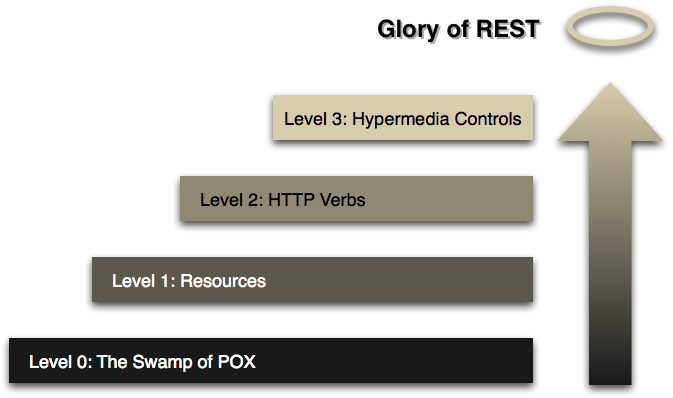
\includegraphics[width=0.8\textwidth]{rmm.png}
  \caption[Richardson Maturity Model]{Richardson Maturity Model \autocite{Fowler2010}}
  \label{fig:rmm}
\end{figure}

Een API is pas echt RESTful als het niveau 3 van het Richardson Maturity Model bereikt \autocite{Fowler2010}. HATEOAS is een belangrijk onderdeel van RESTful API design en wordt beschouwd als het hoogste niveau van volwassenheid. Echter is het implementeren van HATEOAS niet altijd eenvoudig en kan het extra complexiteit met zich meebrengen. Daarom zullen we in een volgend hoofdstuk grondig analyseren of de voordelen van HATEOAS opwegen tegen de nadelen in onze specifieke situatie.

\section{HATEOAS}

HATEOAS (Hypermedia as the Engine of Application State) is een belangrijk onderdeel van RESTful API design en vertegenwoordigt het hoogste niveau van volwassenheid volgens het Richardson Maturity Model (niveau 3) \autocite{Fowler2010}. Het kernidee achter HATEOAS is dat de server niet alleen data terugstuurt, maar ook hypermedia-links die de client informeren over welke acties mogelijk zijn op de opgevraagde data. Deze links fungeren als een soort "knoppen" in de API, die dynamisch veranderen afhankelijk van de status en rechten van de gebruiker.

\subsection{Werking van HATEOAS}

In een HATEOAS-API bevat elke response, naast de gevraagde data, ook links naar gerelateerde resources en mogelijke acties. Deze links worden meestal weergegeven in een gestandaardiseerd formaat, zoals JSON HAL (Hypertext Application Language) of Siren.

\begin{listing}[H]
  \begin{minted}{json}
  {
    "name": "Lars Salembier",
    "email": "lars.salembier@example.com",
    "_links": {
      "self": { "href": "/users/123" },
      "orders": { "href": "/users/123/orders" },
      "update": { "href": "/users/123", "method": "PUT" }
    }
  }
  \end{minted}
  \caption[Voorbeeld van een JSON HAL response]{Voorbeeld van een JSON HAL response met links naar gerelateerde resources en acties.}
  \label{lst:json_hal_example}
\end{listing}

In dit voorbeeld ziet u een JSON-object dat informatie over een gebruiker bevat. Naast de naam en het e-mailadres bevat het object ook een \texttt{links} sectie. Deze sectie bevat links naar gerelateerde resources, zoals de bestellingen van de gebruiker (\texttt{orders}), en mogelijke acties, zoals het bijwerken van de gebruikersgegevens (\texttt{update}). Elke link heeft een \texttt{href} attribuut dat de URL van de resource of actie specificeert, en optioneel een \texttt{method} attribuut dat de HTTP-methode aangeeft die gebruikt moet worden.

\subsection{Voordelen van HATEOAS}

Het gebruik van HATEOAS biedt verschillende voordelen:

\begin{itemize}
  \item \textbf{Loose Coupling:} Clients zijn minder afhankelijk van hardgecodeerde URI's. Als de serverstructuur verandert, hoeven de clients niet aangepast te worden, zolang de links correct blijven functioneren.
  \item \textbf{Ontdekkingsmogelijkheden:} Clients kunnen de API dynamisch ontdekken door de links in de responses te volgen. Dit vereenvoudigt de integratie en maakt de API meer zelfbeschrijvend.
  \item \textbf{Flexibiliteit:} De server kan de beschikbare acties en resources dynamisch aanpassen, zonder dat clients moeten worden bijgewerkt.
  \item \textbf{Documentatie:} HATEOAS kan de documentatie van de API vereenvoudigen, omdat de links zelf al informatie geven over de mogelijke acties en resources.
\end{itemize}

\subsection{Nadelen van HATEOAS}

\begin{itemize}
  \item \textbf{Complexiteit:} Het implementeren van HATEOAS kan complex zijn, vooral bij het ontwerpen van de API en het genereren van de juiste links.
  \item \textbf{Performance:} Het toevoegen van hypermedia-links aan elke response kan de performance van de API beïnvloeden, vooral bij grote datasets.
  \item \textbf{Overhead:} Het toevoegen van hypermedia-links aan elke response kan de grootte van de responses vergroten, wat kan leiden tot overhead.
  \item \textbf{Vendor Lock-in:} Het gebruik van HATEOAS kan leiden tot vendor lock-in, omdat clients afhankelijk zijn van de specifieke implementatie van de API.
  \item \textbf{Beveiliging:} Het toevoegen van hypermedia-links kan beveiligingsrisico's met zich meebrengen, zoals het blootstellen van gevoelige informatie.
  \item \textbf{Caching:} Het cachen van responses kan moeilijker zijn, omdat de links dynamisch gegenereerd worden.
\end{itemize}

\section{OpenAPI}

OpenAPI (voorheen bekend als Swagger) is een specificatie voor het beschrijven van RESTful API's in een machine-leesbaar formaat, meestal YAML of JSON \autocite{OpenAPIInitiative2021}. Het biedt een gestandaardiseerde manier om de structuur en functionaliteit van een API te documenteren, inclusief endpoints, parameters, request bodies, response bodies, authenticatiemethoden en meer. Deze documentatie kan vervolgens gebruikt worden voor diverse doeleinden, zoals het genereren van interactieve API documentatie, het automatisch genereren van client- en servercode, en het testen van de API.

\subsection{Structuur van een OpenAPI document}

Een OpenAPI document bevat verschillende secties die de API beschrijven:

\begin{itemize}
    \item \textbf{openapi:} De OpenAPI specificatie versie.
    \item \textbf{info:} Metadata over de API, zoals de titel, beschrijving en versie.
    \item \textbf{servers:} Een lijst van servers waar de API beschikbaar is.
    \item \textbf{paths:} De endpoints van de API, inclusief de ondersteunde HTTP-methoden en parameters.
    \item \textbf{components:} Herbruikbare componenten, zoals schemas (datatypes) en security schemes.
    \item \textbf{security:} De beveiligingsmechanismen die gebruikt worden door de API.
    \item \textbf{tags:} Tags om de API te categoriseren.
    \item \textbf{externalDocs:} Links naar externe documentatie.
\end{itemize}

\begin{listing}[H]
\begin{minted}{yaml}
openapi: 3.0.0
info:
  title: BrightEats API
  version: v1
paths:
  /orders:
    get:
      summary: Haal alle bestellingen op
      responses:
        '200':
          description: Lijst met bestellingen
          content:
            application/json:
              schema:
                type: array
                items:
                  $ref: '#/components/schemas/Order'
components:
  schemas:
    Order:
      type: object
      properties:
        id:
          type: integer
        description:
          type: string
\end{minted}
\caption[Voorbeeld van een OpenAPI document in YAML]{Voorbeeld van een OpenAPI document in YAML dat een endpoint beschrijft om bestellingen op te halen.}
\label{lst:openapi_example}
\end{listing}


\subsection{Tools voor OpenAPI}

Er zijn verschillende tools beschikbaar die werken met OpenAPI-documenten:

\begin{itemize}
  \item \textbf{Swagger UI:} Genereert interactieve documentatie waarmee gebruikers de API kunnen verkennen en testen.
  \item \textbf{Redoc:} Genereert statische documentatie in een aantrekkelijke en leesbare vorm.
  \item \textbf{OpenAPI Generator:} Genereert client- en servercode in verschillende programmeertalen op basis van een OpenAPI document.
  \item \textbf{Postman:} Ondersteunt het importeren en exporteren van OpenAPI-documenten en kan gebruikt worden voor het testen van de API.
\end{itemize}

\subsection{Voordelen van OpenAPI}

\begin{itemize}
  \item \textbf{Gestandaardiseerde documentatie:} OpenAPI biedt een gestandaardiseerde manier om API's te documenteren, waardoor de documentatie consistent en gemakkelijk te begrijpen is.
  \item \textbf{Automatische documentatiegeneratie:} Tools zoals Swagger UI en Redoc kunnen automatisch documentatie genereren op basis van een OpenAPI-document, waardoor de documentatie altijd up-to-date is.
  \item \textbf{Codegeneratie:} OpenAPI Generator kan client- en servercode genereren in verschillende programmeertalen, waardoor ontwikkeltijd wordt bespaard.
  \item \textbf{Testen:} OpenAPI-documenten kunnen gebruikt worden voor het automatisch testen van de API.
  \item \textbf{Samenwerking:} OpenAPI vergemakkelijkt de samenwerking tussen frontend- en backend-teams door een duidelijke en gedeelde specificatie van de API te bieden.
\end{itemize}

\subsection{Nadelen van OpenAPI}

\begin{itemize}
  \item \textbf{Leercurve:} Het leren schrijven en onderhouden van OpenAPI-documenten vereist enige inspanning.
  \item \textbf{Onderhoud:} OpenAPI documenten moeten up-to-date gehouden worden met de API, wat extra onderhoud vereist. Dit kan echter ook als een voordeel worden beschouwd, omdat het dwingt tot het consistent documenteren van de API.
\end{itemize}

\section{HATEOAS: Een evaluatie voor BrightAnalytics}

HATEOAS (Hypermedia as the Engine of Application State) vertegenwoordigt het hoogste niveau van volwassenheid binnen RESTful API design volgens het Richardson Maturity Model (niveau 3) \autocite{Fowler2010}. In dit hoofdstuk evalueren we de toepasbaarheid van HATEOAS binnen de specifieke context van BrightAnalytics. Hoewel HATEOAS theoretisch voordelen biedt, zullen we aantonen dat de implementatie ervan in onze situatie niet gerechtvaardigd is.

\subsection{Baten}

HATEOAS beidt clients de mogelijkheid om een API dynamisch te ontdekken en te navigeren zonder voorafgaande kennis van de URI-structuur. Elke response bevat hypermedia-links die de client informeren over de beschikbare acties en gerelateerde resources. Dit biedt potentiële voordelen zoals:

\begin{itemize}
  \item \textbf{Loose Coupling:} Clients zijn minder afhankelijk van hardgecodeerde URI's, waardoor de serverstructuur kan evolueren zonder directe impact op de clients.
  \item \textbf{Ontdekkingsmogelijkheden:} Clients kunnen de API dynamisch verkennen door de aangeboden links te volgen.
  \item \textbf{Flexibiliteit:} De server kan de beschikbare acties en resources dynamisch aanpassen.
\end{itemize}

\subsection{Kosten}

Een cruciaal aspect van onze situatie is dat de te ontwikkelen API's uitsluitend intern gebruikt zullen worden binnen BrightAnalytics. Dit betekent dat de development teams directe toegang hebben tot uitgebreide documentatie en effectief kunnen communiceren over de API-structuur. De noodzaak voor de ontdekkingsmogelijkheden die HATEOAS biedt, wordt hierdoor sterk gereduceerd.

\bigskip

De implementatie van HATEOAS brengt aanzienlijke kosten met zich mee, die in onze context niet opwegen tegen de beperkte voordelen.

\bigskip

Het genereren en beheren van hypermedia-links introduceert extra complexiteit in de ontwikkeling van de API. Dit vereist een doordachte implementatie en grondig testen om de correctheid en consistentie van de links te garanderen.

\bigskip

Het toevoegen van hypermedia-links aan elke response vergroot de hoeveelheid data die verzonden moet worden. Dit kan een negatieve impact hebben op de performance, met name bij grote datasets.

\bigskip

Gezien de interne context en de reeds aanwezige communicatiekanalen binnen de development teams, is de meerwaarde van HATEOAS beperkt. De kosten van implementatie en onderhoud wegen niet op tegen de minimale winst in ontdekkingsmogelijkheden.

\bigskip

De ontwikkeling van de API's zal gepaard gaan met uitgebreide documentatie gebaseerd op de OpenAPI specificatie. Met behulp van tools zoals Swagger UI of Redoc zal deze documentatie interactief en gemakkelijk toegankelijk zijn voor alle betrokken developers. Dit biedt een effectief alternatief voor de ontdekkingsmogelijkheden van HATEOAS, zonder de bijbehorende complexiteit en overhead.

\subsection{Conclusie}

Gezien de interne context van de API's bij BrightAnalytics en de beschikbaarheid van uitgebreide OpenAPI documentatie, concluderen we dat de implementatie van HATEOAS niet gerechtvaardigd is. De kosten en complexiteit wegen niet op tegen de beperkte voordelen. Daarom kiezen we ervoor om HATEOAS niet te implementeren in onze API's.

\section{RESTful API best practices en de Zalando Guidelines}

Het ontwerpen en implementeren van hoogwaardige, onderhoudbare en schaalbare RESTful API's vereist het volgen van best practices. Hoewel een gedetailleerde bespreking van alle best practices buiten het bestek van deze literatuurstudie valt, erkennen we het belang ervan en zullen we een set specifieke richtlijnen opstellen tijdens de ontwikkelingsfase van onze API's. Hierbij zullen we ons baseren op de uitgebreide \textit{Zalando RESTful API Guidelines} \autocite{ZAG2024}.

\subsection{De Zalando RESTful API Guidelines}

De Zalando RESTful API Guidelines bieden een uitgebreid framework voor het ontwerpen en ontwikkelen van RESTful API's. Deze guidelines behandelen een breed scala aan onderwerpen, waaronder:

\begin{itemize}
  \item \textbf{URI Design:} Richtlijnen voor het creëren van consistente, leesbare en betekenisvolle URI's.
  \item \textbf{HTTP Methoden:} Correct gebruik van HTTP methoden (GET, POST, PUT, PATCH, DELETE) en hun semantische betekenis.
  \item \textbf{Status Codes:} Gebruik van de juiste HTTP status codes om de uitkomst van requests te communiceren.
  \item \textbf{Dataformaten:} Richtlijnen voor het gebruik van de juiste dataformaten.
  \item \textbf{Versionering:} Strategieën voor het beheren van API versies en het waarborgen van backward compatibility.
  \item \textbf{Foutbehandeling:} Best practices voor het afhandelen en rapporteren van fouten.
  \item \textbf{Authenticatie en Autorisatie:} Beveiligingsmechanismen voor het beschermen van de API.
  \item \textbf{Documentatie:} Het belang van duidelijke en complete API documentatie.
  \item \textbf{Paginering:} Technieken voor het efficiënt verwerken van grote datasets.
  \item \textbf{Filtering en Sortering:} Mogelijkheden voor clients om data te filteren en te sorteren.
\end{itemize}

De Zalando RESTful API Guidelines bieden een waardevolle bron van best practices en richtlijnen voor het ontwerpen van RESTful API's. We zullen deze guidelines gebruiken als basis voor het opstellen van onze eigen set richtlijnen tijdens de ontwikkeling van de BrightEats API.

\section{Implementatie met Laravel en Vue.js}

Dit hoofdstuk beschrijft de gekozen technologieën voor de backend en frontend ontwikkeling, namelijk Laravel en Vue.js, en hoe de concepten van RESTful API design en OpenAPI daarop worden toegepast.

\subsection{Laravel als backend framework}

Laravel is een populair PHP framework dat zich uitstekend leent voor het ontwikkelen van robuuste en schaalbare webapplicaties, inclusief RESTful API's. We kiezen voor Laravel vanwege de volgende redenen \autocite{Laravel}:

\begin{itemize}
  \item \textbf{MVC Architectuur:} Laravel's Model-View-Controller architectuur bevordert een gestructureerde en modulaire codebase, wat de ontwikkeling en onderhoudbaarheid van API's vereenvoudigt.
  \item \textbf{Eloquent ORM:} De Eloquent ORM (Object-Relational Mapper) maakt het eenvoudig om te interageren met databases en data te manipuleren.
  \item \textbf{Routing:} Laravel biedt een flexibel en krachtig routing systeem voor het definiëren van API endpoints.
  \item \textbf{Middleware:} Middleware in Laravel kan gebruikt worden voor taken zoals authenticatie, autorisatie, logging en request validatie.
  \item \textbf{Testing:} Laravel biedt uitgebreide mogelijkheden voor het testen van API's.
  \item \textbf{Community en Documentatie:} Laravel heeft een grote en actieve community en uitgebreide documentatie, wat de ontwikkeling vergemakkelijkt.
\end{itemize}

\subsubsection{RESTful API's in Laravel}

Laravel biedt ingebouwde ondersteuning voor het ontwikkelen van RESTful API's. Resources kunnen worden gedefinieerd met behulp van resource controllers en routes.

\begin{listing}[H]
\begin{minted}{php}
  use App\Models\Product;
  use Illuminate\Http\Request;
  use App\Http\Resources\ProductResource;
  
  class ProductController extends Controller
  {
    public function index()
    {
      return ProductResource::collection(Product::all());
    }

    public function show(Product $product)
    {
      return new ProductResource($product);
    }

    public function store(Request $request)
    {
      $validated = $request->validate([
        'name' => 'required|max:255',
        'price' => 'required|numeric',
      ]);

      $product = Product::create($validated);

      return new ProductResource($product);
    }

    // ... update, destroy methods ...
  }
\end{minted}
\caption[Voorbeeld van een Laravel resource controller]{Voorbeeld van een Laravel resource controller voor het beheren van producten.}
\label{lst:laravel_controller}
\end{listing}

\subsection{Vue.js als frontend framework}

Vue.js is een progressief JavaScript framework dat ideaal is voor het bouwen van interactieve user interfaces \autocite{VueJS}. We kiezen voor Vue.js vanwege:

\begin{itemize}
  \item \textbf{Component-gebaseerde architectuur:} Vue.js stimuleert het ontwikkelen van herbruikbare componenten, wat de codebase overzichtelijker en onderhoudbaarder maakt.
  \item \textbf{Reactiviteit:} Vue.js' reactieve data binding zorgt ervoor dat de user interface automatisch wordt bijgewerkt wanneer de data verandert.
  \item \textbf{Eenvoudige integratie:} Vue.js kan gemakkelijk geïntegreerd worden met andere libraries en frameworks.
  \item \textbf{Performance:} Vue.js is lightweight en performant.
  \item \textbf{Community en Documentatie:} Net als Laravel heeft Vue.js een grote en actieve community en uitgebreide documentatie.
\end{itemize}

\subsubsection{Consumptie van de API in Vue.js}

Vue.js-applicaties kunnen de Laravel API consumeren met behulp van HTTP clients zoals Axios of de ingebouwde Fetch API. Data opgehaald van de API kan vervolgens gebruikt worden om de user interface dynamisch te vullen.

\begin{listing}[H]
\begin{minted}{javascript}
  <template>
  <ul>
    <li v-for="product in products" :key="product.id">
      {{ product.name }} - {{ product.price }}
    </li>
  </ul>
  </template>

  <script>
  import axios from 'axios';

  export default {
  data() {
    return {
      products: [],
    };
  },
  mounted() {
    axios.get('/api/products')
      .then(response => {
        this.products = response.data.data;
      })
      .catch(error => {
        console.error(error);
      });
  },
  };
  </script>
\end{minted}
\caption[Voorbeeld van het ophalen van data van een Laravel API in Vue.js]{Voorbeeld van het ophalen van data van een Laravel API in Vue.js met behulp van Axios.}
\label{lst:vue_axios}
\end{listing}

\subsection{OpenAPI integratie}

OpenAPI zal een centrale rol spelen in de ontwikkeling van onze API's. We zullen een OpenAPI-document creëren dat de API volledig beschrijft. Dit document zal dienen als basis voor:

\begin{itemize}
  \item \textbf{Documentatie:} Automatische generatie van interactieve documentatie met behulp van tools zoals Swagger UI.
  \item \textbf{Client code generatie:} Mogelijkheid om client code te genereren in verschillende talen.
  \item \textbf{Server side validatie:} Validatie van requests en responses op basis van het OpenAPI schema.
  \item \textbf{Testing:} Automatische tests genereren op basis van het OpenAPI document.
\end{itemize}

Door OpenAPI te integreren in ons ontwikkelproces, zorgen we voor een consistente, goed gedocumenteerde en gemakkelijk te onderhouden API.

\begin{listing}[H]
\begin{minted}{yaml}
paths:
  /products:
    get:
      summary: Get all products
      responses:
        '200':
          description: A list of products
          content:
            application/json:
              schema:
                type: object
                properties:
                  data:
                    type: array
                    items:
                      $ref: '#/components/schemas/Product'
components:
  schemas:
    Product:
      type: object
      properties:
        id:
          type: integer
          readOnly: true
        name:
          type: string
        price:
          type: number
          format: float
\end{minted}
\caption[Voorbeeld van een OpenAPI document in YAML]{Voorbeeld van een OpenAPI document in YAML dat een endpoint beschrijft om producten op te halen.}
\label{lst:openapi_example_resource}
\end{listing}

\section{Conclusie}

Deze literatuurstudie heeft een overzicht geboden van de belangrijkste concepten en technologieën die relevant zijn voor het ontwikkelen van robuuste, schaalbare en goed gedocumenteerde RESTful API's, met specifieke aandacht voor de context van BrightAnalytics en hun bestaande technologie stack. We begonnen met een inleiding tot API's in het algemeen, waarna we de principes van RESTful API design hebben geanalyseerd, inclusief de zes belangrijkste principes (Client-Server, Stateless, Cacheable, Uniform Interface, Layered System en Code-On-Demand), HTTP methoden, status codes en het resource-gebaseerde karakter van REST.

\bigskip

Vervolgens introduceerden we het Richardson Maturity Model, dat de volwassenheid van RESTful API's beschrijft, met speciale aandacht voor HATEOAS. Na een grondige evaluatie van de voor- en nadelen van HATEOAS, in combinatie met de specifieke context van BrightAnalytics - interne API's en een nadruk op heldere documentatie - concludeerden we dat de implementatie van HATEOAS voor dit project niet de meest efficiënte aanpak is. De complexiteit en overhead wegen niet op tegen de beperkte voordelen in onze situatie. Deze beslissing wordt versterkt door onze keuze voor OpenAPI, waarmee we uitgebreide en interactieve documentatie zullen genereren, wat de noodzaak voor de ontdekkingsaspecten van HATEOAS minimaliseert.

\bigskip

OpenAPI vormt een kerncomponent in onze API-ontwikkelingsstrategie. Door een OpenAPI-document te creëren dat de API volledig beschrijft, waarborgen we consistente documentatie, automatische codegeneratie, server-side validatie en geautomatiseerd testen. Dit bevordert de kwaliteit, onderhoudbaarheid en schaalbaarheid van onze API's. De integratie van OpenAPI, gecombineerd met de techstack van BrightAnalytics (Laravel en Vue.js), optimaliseert ons ontwikkelproces.

\bigskip

Ten slotte benadrukten we het belang van best practices voor API-ontwikkeling. Een gedetailleerde beschrijving hiervan valt buiten het bestek van deze literatuurstudie, maar tijdens de ontwikkeling zullen we specifieke richtlijnen formuleren, gebaseerd op de Zalando RESTful API Guidelines. Dit framework biedt een solide basis voor het ontwerpen en implementeren van RESTful API's, waarmee we de consistentie, betrouwbaarheid en schaalbaarheid van onze API's willen verhogen.

%%=============================================================================
%% Methodologie
%%=============================================================================

\chapter{\IfLanguageName{dutch}{Methodologie}{Methodology}}%
\label{ch:methodologie}

Deze bachelorproef onderzoekt en verbetert de API-kwaliteit bij BrightAnalytics door de iteratieve ontwikkeling van de BrightEats API. Onderzoek en ontwikkeling gaan hand in hand. De inzichten uit het onderzoek worden direct toegepast op de API, en de ervaringen tijdens de ontwikkeling sturen het onderzoek bij.

Ik ga ervan uit dat ik elke week minstens \'e\'en dag kan werken aan de bachelorproef. De deadlines zijn echter flexibel, aangezien de API-ontwikkeling continu doorloopt en de planning kan be\"invloeden.

Na evaluatie in de literatuurstudie blijkt implementatie van HATEOAS niet geschikt voor de BrightEats API. In plaats daarvan focussen we op het opstellen van een interne guide, gebaseerd op best practices en vergelijkbaar met de Zalando RESTful API and Event Scheme Guidelines. Daarnaast wordt een uitgebreide OpenAPI-specificatie voor de API ontwikkeld.

\section{Fase 1: Onderzoek en eerste opzet API}

\textbf{Deadline: 17 november 2024}

Deze fase is gericht op het verzamelen van kennis over kwalitatieve API-ontwikkeling en het defini\"eren van een eerste set best practices voor BrightEats. Ik bestudeer de principes van REST, HATEOAS en OpenAPI en hun belang voor API-kwaliteit en formuleer concrete aanbevelingen voor de BrightEats API.

\bigskip

\textbf{We zoeken een antwoord op de volgende vragen:}
\begin{itemize}
  \item Wat zijn de principes van REST?
  \item Hoe dragen deze bij aan betere API's?
  \item Welke best practices zijn er voor URI-structuur, HTTP-methoden, response codes en versiebeheer?
  \item Hoe houden we onze Laravel-API RESTful?
  \item Wat zijn de principes en voordelen van HATEOAS?
  \item Hoe kunnen we HATEOAS implementeren in een Laravel-API?
  \item Hoe maken we optimaal gebruik van HATEOAS in de frontend van BrightEats?
  \item Wat is OpenAPI en hoe kan dit worden toegepast in de documentatie van een Laravel-API?
\end{itemize}

\textbf{Deliverables:}

\begin{itemize}
  \item Literatuurstudie over REST, HATEOAS en OpenAPI.
  \item Best practices voor de implementatie in de BrightEats API en frontend.
\end{itemize}

\section{Fase 2: Iteratieve ontwikkeling en verfijning BrightEats API}

\textbf{Deadline: 8 december 2024}

\bigskip
Gedurende deze fase refactor ik de BrightEats API iteratief naar een RESTful design, terwijl we ook de OpenAPI-specificatie definiëren. We doen dit stap per stap, zonder de hele API in één keer te herschrijven. De focus ligt op het toepassen van de best practices die we in fase 1 hebben geformuleerd.

\subsection{Ontwikkeling van de API (doorlopend)}

\bigskip
Elke week doorloop ik de volgende stappen:

\begin{enumerate}
  \item \textbf{Plannen:} Ik bepaal welke functionaliteiten ik aan de API zal toevoegen (of welke code ik ga refactoren om zo aan de nieuwe best practices te voldoen)
  \item \textbf{Ontwerpen:} Ik ontwerp de nieuwe/gerefactorde functionaliteiten met de best practices in gedachten.
  \item \textbf{Implementeren:} Ik programeer de nieuwe/gerefactorde functionaliteiten in de API.
  \item \textbf{Testen:} Ik test de nieuwe/gerefactorde functionaliteiten grondig.
  \item \textbf{Evalueren:} Ik beoordeel de kwaliteit, structuur en gebruikte best practices.
  \item \textbf{Best practices bijstellen:} Ik pas de richtlijnen aan op basis van de evaluatie en feedback.
\end{enumerate}

\textbf{Deliverables:}

\begin{itemize}
  \item Een concrete set best practices voor de BrightEats API.
  \item De API zelf, volgens de best practices.
\end{itemize}

\section{Fase 3: Synthese, aanbevelingen en afronding}

\textbf{Deadline: 15 december 2025}

\bigskip
In de laatste fase vat ik mijn bevindingen samen en formuleer ik een antwoord op de onderzoeksvraag. Wat was de exacte kost van het implementeren van OpenAPI en RESTfulness in de BrightEats API? Welke voordelen en nadelen bracht dit met zich mee? Welke best practices kunnen we formuleren voor de ontwikkeling van API's bij BrightAnalytics?

\subsection{Synthese \& Aanbevelingen}

\textbf{Deadline: 15 januari 2025}

\bigskip
Ik schrijf de conclusie en aanbevelingen voor BrightAnalytics. Hierbij beantwoord ik de deelvragen en onderzoeksvraag en formuleer ik concrete best practices voor de ontwikkeling van RESTful API's bij BrightAnalytics.

\subsection{Afronding bachelorproef}

\textbf{Deadline: 10 januari 2025}

\bigskip
Ik werk de bachelorproef af, rekening houdend met de feedback van de promotor en de copromotor bij BrightAnalytics.

\textbf{Deliverables:}

\begin{itemize}
  \item Concrete aanbevelingen voor beter API-ontwerp.
  \item Finale versie van de bachelorproef.
\end{itemize}

\section{Gantt chart}

\begin{figure}[H]
  \centering
  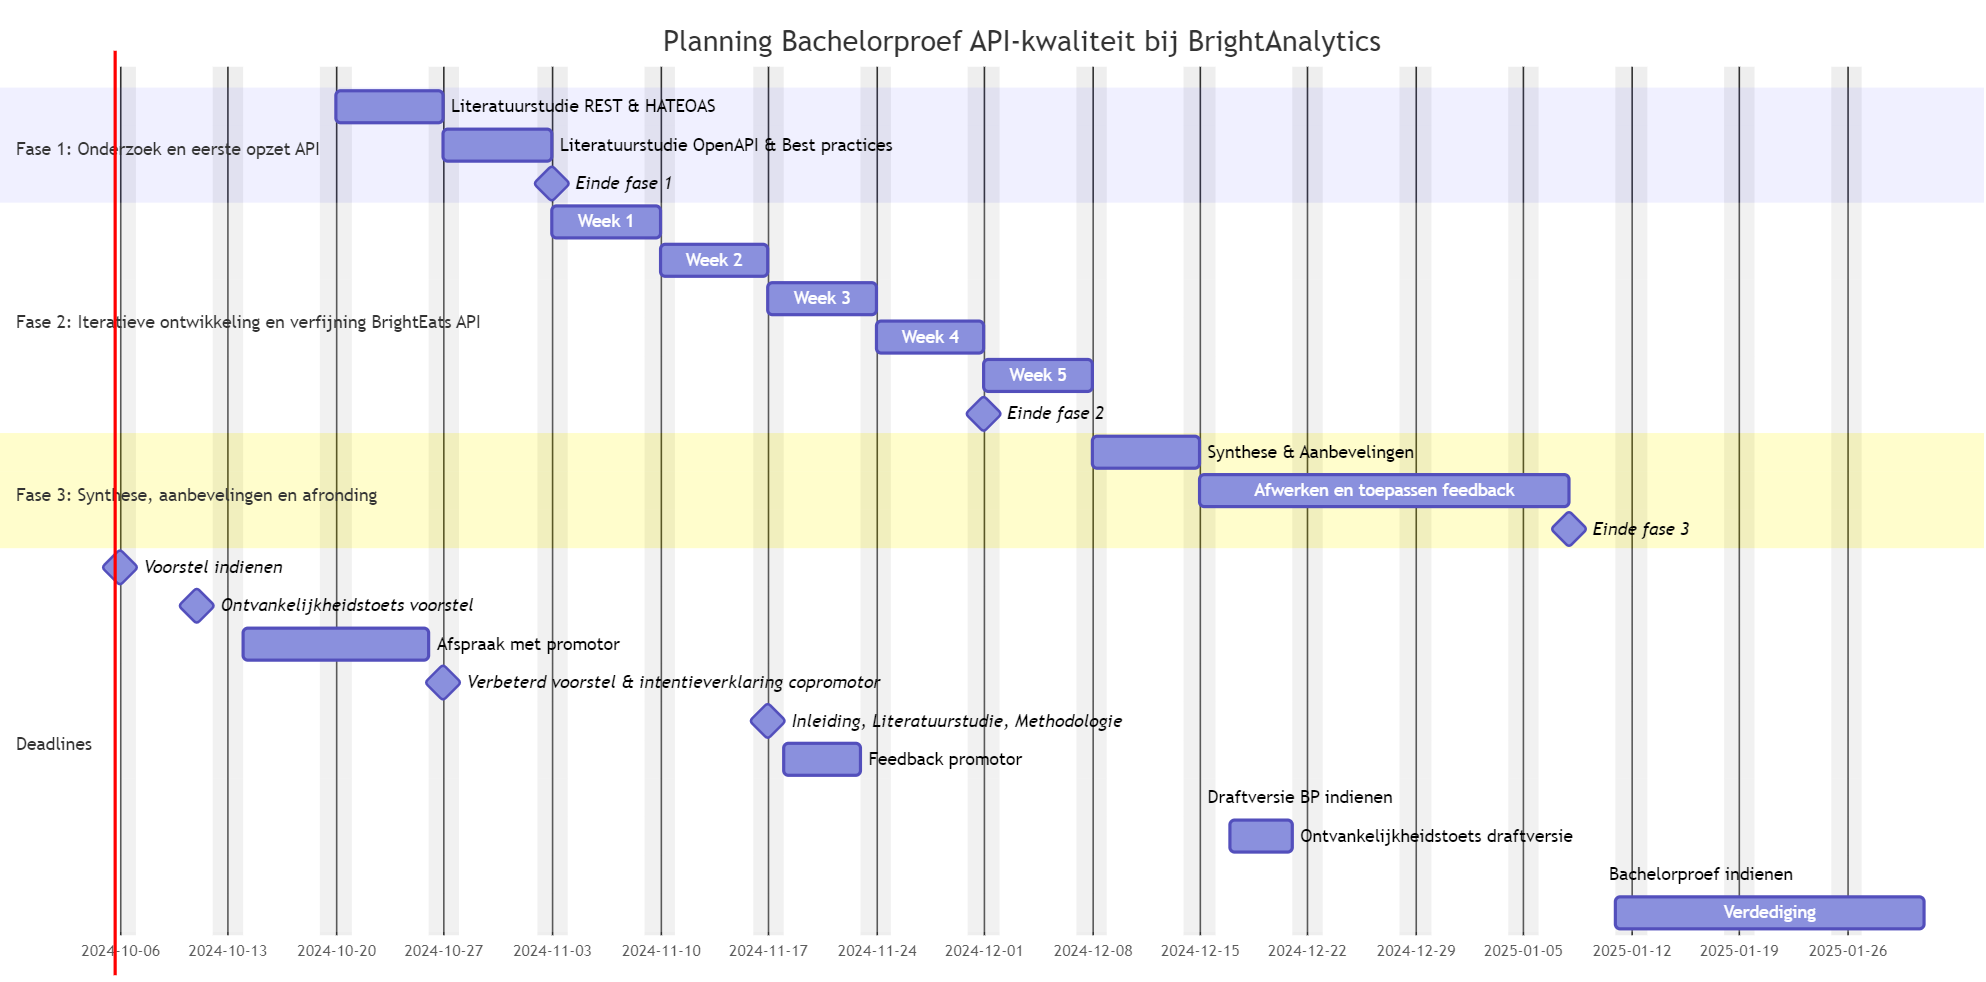
\includegraphics[width=0.8\textwidth]{gantt.png}
  \caption{Gantt chart van de methodologie}
  \label{fig:gantt}
\end{figure}


% Voeg hier je eigen hoofdstukken toe die de ``corpus'' van je bachelorproef
% vormen. De structuur en titels hangen af van je eigen onderzoek. Je kan bv.
% elke fase in je onderzoek in een apart hoofdstuk bespreken.

\chapter{Richtlijnen}
\label{ch:richtlijnen}

Deze richtlijnen zijn opgesteld om de consistentie, kwaliteit en onderhoudbaarheid van RESTful API's binnen BrightAnalytics te waarborgen. Ze zijn gebaseerd op de Zalando RESTful API Guidelines \autocite{ZAG2024} en aangepast aan de specifieke context van BrightAnalytics.

\section{Principes}

Een RESTful API heeft als doel om resources te modelleren en toegankelijk te maken via een uniforme interface. Ze kunnen ge\"identificeerd via URI's en kunnen aangepast worden via gestandaardiseerde HTTP-methoden (GET, POST, PUT, PATCH, DELETE).

\bigskip

De API moet consistent, voorspelbaar en gemakkelijk te gebruiken zijn voor ontwikkelaars. Dit betekent dat URI's, HTTP-methoden, statuscodes en dataformaten consistent en goed gedocumenteerd moeten zijn.

\bigskip

Een belangrijk principe is de Wet van Postel, ook bekend als het Robustness Principle: ``Wees conservatief in wat je stuurt, en liberaal in wat je ontvangt''. Dit betekent dat de API tolerant moet zijn ten opzichte van variaties in input, maar dat de output consistent en voorspelbaar moet zijn.

\section{Algemeen}

\subsection{Elke API moet gedocumenteerd worden met OpenAPI}
\label{section:openapi_documentatie}

Hierbij is het zeker toegelaten om tools te gebruiken die de OpenAPI-specificatie genereren op basis van de code, zoals Swagger UI of Redoc. Dit zorgt voor een consistente en gemakkelijk toegankelijke documentatie voor ontwikkelaars. Voor Laravel gebruiken we de package \texttt{dedoc/scramble} om de OpenAPI-specificatie te genereren en te renderen.

\subsection{Elke API moet een handleiding bevatten}
\label{section:api_handleiding}

Naast de API-specificatie is het belangrijk om een handleiding te voorzien die de API beschrijft, inclusief voorbeelden en best practices. Deze handleiding bevindt zich meestal in de \texttt{README} van de repository. Deze bevat zeker de volgende informatie:

\begin{itemize}
    \item De scope van de API, samen met het nut ervan en de use cases.
    \item Concrete voorbeelden van het gebruik van de API.
    \item Edge cases, wat te doen bij foutmeldingen en veelvoorkomende problemen en oplossingen.
    \item Informatie over authenticatie en autorisatie.
    \item Informatie over versiebeheer en migratie.
    \item De algemene architectuur van de API en de gebruikte technologieën.
\end{itemize}

\subsection{API's moeten geschreven worden in Amerikaans Engels}
\label{section:amerikaans_engels}

Dit om consistentie te garanderen en het gemakkelijker te maken voor ontwikkelaars om de API te begrijpen.

\section{REST - Meta-informatie}

\subsection{De OpenAPI-specificatie moet meta-informatie bevatten}
\label{section:openapi_meta_informatie}

De OpenAPI-specificatie bevat minstens de volgende meta-informatie:

\begin{itemize}
    \item \texttt{\#/info/title}: De naam van de API. Deze moet uniek, beschrijvend en gemakkelijk te begrijpen zijn.
    \item \texttt{\#/info/version}: De versie van de API. Dit is belangrijk voor versiebeheer en migratie. We gebruiken hierbij semantic versioning (SemVer), zie \ref{subsection:semantic_versioning}.
    \item \texttt{\#/info/description}: Een korte maar duidelijke beschrijving van de API en zijn doel en scope.
    \item \texttt{\#/info/contact/{name,url,email}}: Contactinformatie voor de ontwikkelaars van de API.
\end{itemize}

\subsection{De API moet semantic versioning gebruiken}
\label{subsection:semantic_versioning}

Semantic versioning (SemVer) is een conventie voor het versiebeheer van software. Het bestaat uit drie getallen, gescheiden door punten: \texttt{MAJOR.MINOR.PATCH}. Bij elke wijziging in de API moet minstens één van deze cijfers verhoogd worden:

\begin{itemize}
    \item \textbf{MAJOR}: Verhoog bij incompatibele wijzigingen in de API.
    \item \textbf{MINOR}: Verhoog bij toevoeging van nieuwe functionaliteit in een backwards-compatible manier.
    \item \textbf{PATCH}: Verhoog bij backwards-compatible bugfixes die de functionaliteit niet uitbreiden.
\end{itemize}

Vooraleer de API in productie gaat, zal de versie steeds \texttt{0.x.y} zijn. Dit betekent dat de API nog in ontwikkeling is en dat er nog geen garanties zijn over de stabiliteit van de API. Wanneer de API klaar is voor productie, zal de versie verhoogd worden naar \texttt{1.0.0}.

\section{REST - Beveiliging}

\subsection{Endpoints moeten beveiligd zijn}
\label{section:beveiligde_endpoints}

Alle endpoints moeten beschermd worden met authenticatie en autorisatie. De keuze van de methode hangt af van de use case en de gevoeligheid van de data. Mogelijkheden zijn bearer tokens, API keys, OAuth 2.0, en JWT.

\section{REST - Dataformaten}

\subsection{De API moet standaard dataformaten gebruiken}
\label{section:standaard_dataformaten}

OpenAPI definieert standaard dataformaten voor de meeste datatypes. Deze moeten gebruikt worden om de consistentie en voorspelbaarheid van de API te garanderen. Hiervoor verwijs ik naar de tabel in guideline 238 van de Zalando RESTful API Guidelines \autocite{ZAG2024}.

\subsection{De API moet een formaat voor getallen en integers gebruiken.}
\label{section:formaat_getallen_integers}

Specifieer steeds een formaat \texttt{int32}, \texttt{int64}, of \texttt{bigint} voor \texttt{integer} waarden en \texttt{float}, \texttt{double}, of \texttt{decimal} voor \texttt{number} waarden. Op die manier moeten clients niet raden welk formaat gebruikt wordt en kunnen ze de data correct verwerken, zonder verlies van precisie.

\bigskip

Client en server moeten de dataformaten zo specifiek mogelijk vertalen naar hun eigen datastructuren. Bijvoorbeeld, het type \texttt{number} met formaat \texttt{double} in OpenAPI kan vertaald worden naar een \texttt{double} in Java of een \texttt{float64} in Go.

\subsection{De API moet binaire data als \texttt{base64url} coderen.}
\label{section:binaire_data_base64url}

Je moet eerst proberen om binaire data te vermijden in API's. Als dit niet mogelijk is, moet je binaire data als \texttt{base64url} coderen volgens \textcite{rfc7493}. Dit zorgt ervoor dat de data correct verwerkt kan worden door clients en dat er geen data verloren gaat.

Binaire data kan vermeden worden door de data terug te geven met een standaard media type, zoals \texttt{image/png} of \texttt{application/pdf}. Dit is meestal de beste oplossing, omdat het de grootte van de response vermindert en de data correct kan verwerkt worden door clients.

\subsection{De API moet een formaat voor datum en tijd gebruiken.}
\label{section:formaat_datum_tijd}

Gebruik de standaard formaten \texttt{date}, \texttt{date-time}, \texttt{time}, \texttt{duration}, en \texttt{period} voor datum en tijd waarden. Dit zorgt voor consistentie en voorspelbaarheid in de API.

\bigskip

Gebruik de hoofdletter \texttt{T} als scheidingsteken tussen datum en tijd, en de hoofdletter \texttt{Z} voor het aanduiden van Zulu time. Dit is niet verplicht volgens \textcite{rfc3339}, maar het is een veelgebruikte conventie en zorgt ervoor dat responses voorspelbaarder zijn.

\bigskip

De standaard laat time zone offsets toe, maar deze kunnen verwarrend zijn en zijn niet altijd nodig. Gebruik enkel time zone offsets als het nodig is voor de use case. Als je time zone offsets gebruikt, gebruik dan de \texttt{Z} notatie voor Zulu time (UTC) en de \texttt{+HH:MM} notatie voor andere tijdzones. Voor het opslaan van de data in een databank gebruiken we verplicht altijd UTC-tijd.

\bigskip

Gebruik geen numerieke timestamps. Numerieke timestamps kunnen problemen veroorzaken met precisie. Gebruik altijd een datum- en tijdformaat.

\subsection{De API moet een goede keuze maken tussen \texttt{date} en \texttt{date-time}.}
\label{section:keuze_date_date_time}

Bij het kiezen tussen \texttt{date} en \texttt{date-time}, moet je rekening houden met de volgende zaken:

\begin{itemize}
    \item \texttt{date}: Gebruik \texttt{date} als enkel de datum belangrijk is en de tijd niet relevant is. Bijvoorbeeld: geboortedatum, startdatum, einddatum. Zonder extra context bedoelen we met \texttt{date} altijd de volledige dag, van middernacht tot middernacht, in de lokale tijdzone. De tijdzone kan echter ook gedefineerd worden door de context van de API, zoals bijvoorbeeld een ander veld dat een locatie bevat.
    \item \texttt{date-time}: Gebruik \texttt{date-time} als zowel de datum als de tijd belangrijk zijn. Hier is het meegeven van een tijdzone verplicht, en geven we de voorkeur aan UTC-tijd. Bijvoorbeeld: een afspraak, een deadline, een event.
\end{itemize}

\subsection{De API moet standaardformaten gebruiken voor tijdsduur en tijdsinterval.}
\label{section:standaardformaten_tijdsduur_tijdsinterval}

Gebruik de standaardformaten \texttt{duration} en \texttt{period} voor tijdsduur en tijdsinterval waarden. Dit zorgt voor consistentie en voorspelbaarheid in de API. We gebruiken hierbij ook de \textcite{rfc3339} notatie die open-ended intervals ondersteunt. Dit is de syntax voor \texttt{duration} en \texttt{period} in ANBF:

\begin{minted}{text}
  <dur-second>        ::= [0-9]+S
  <dur-minute>        ::= [0-9]+M <dur-second>?
  <dur-hour>          ::= [0-9]+H <dur-minute>?
  <dur-time>          ::= T<dur-hour> | T<dur-minute> | T<dur-second>
  <dur-day>           ::= [0-9]+D
  <dur-week>          ::= [0-9]+W
  <dur-month>         ::= [0-9]+M <dur-day>?
  <dur-year>          ::= [0-9]+Y <dur-month>?
  <dur-date>          ::= <dur-year> <dur-time>? | <dur-month> <dur-time>? | <dur-day> <dur-time>?
  <duration>          ::= P<dur-date> | P<dur-time> | P<dur-week>

  <period-explicit>   ::= <iso-date-time>/<iso-date-time>
  <period-start>      ::= <iso-date-time>/<duration> | -- startdatum en duur
                          <iso-date-time/..          | -- zonder einde
  <period-end>        ::= <duration>/<iso-date-time> | -- duur en einddatum
                          ../<iso-date-time>          -- zonder begin
  <period>            ::= <period-explicit> | <period-start> | <period-end>
\end{minted}

Een query parameter die een tijdsinterval representeert, definiëren we als \texttt{<time-property>\_between} en niet als \texttt{<time-property>\_before} en \texttt{<time-property>\_after}. Als we een tijdsinterval teruggeven doen we dit met de naam \texttt{<time-property>\_interval}.

\subsection{De API moet de standaardformaten voor landen, talen en valuta gebruiken.}
\label{section:standaardformaten_landen_talen_valuta}

Gebruik de standaardformaten \texttt{iso-3166-alpha-2} \autocite{iso3166-1}, \texttt{iso-639-1} \autocite{iso639}, en \texttt{iso-4217} \autocite{iso4217} voor landen, talen en valuta. Dit zorgt voor consistentie en voorspelbaarheid in de API.

\subsection{De API moet content negotiation gebruiken voor dataformaten als er meerdere opties zijn.}
\label{section:content_negotiation}

Als er meerdere opties zijn voor dataformaten, zoals JSON, PDF, TEXT of HTML, moet de API content negotiation gebruiken om de voorkeur van de client te bepalen. Hiervoor gebruiken we de volgende HTTP headers:

\begin{itemize}
    \item \texttt{Accept}: De client geeft aan welke content types hij accepteert.
    \item \texttt{Accept-Language}: De client geeft aan welke talen hij accepteert.
    \item \texttt{Accept-Encoding}: De client geeft aan welke encodings hij accepteert.
    \item \texttt{Content-Type}: De server geeft aan welk content type hij terugstuurt.
    \item \texttt{Content-Language}: De server geeft aan in welke taal hij terugstuurt.
    \item \texttt{Content-Encoding}: De server geeft aan in welke encoding hij terugstuurt.
\end{itemize}

\section{REST - URL's}

\subsection{De API mag niet \text{/api} als basispad gebruiken.}
\label{section:geen_api_basispad}

Het is niet nodig om \texttt{/api} als basispad te gebruiken voor de API. Het basispad van een API is een kwestie van deployment, en kan dus variëren afhankelijk van de omgeving. Het is beter om het basispad dynamisch te maken, zodat het kan ingesteld worden via een configuratiebestand of een omgevingsvariabele.

\subsection{De API moet zelfstandige naamwoorden in het meervoud gebruiken voor resource collections.}
\label{section:meervoud_resource_collections}

Gebruik zelfstandige naamwoorden in het meervoud voor resource collections. Dit zorgt voor een consistente en voorspelbare URI-structuur. Voorbeelden zijn \texttt{/orders}, \texttt{/users}, \texttt{/shops}.

\subsection{De API moet kebab-case gebruiken voor URI's.}
\label{section:kebab_case_uris}

Gebruik kebab-case om woorden te scheiden in URI-segmenten. Dit zorgt voor een consistente en leesbare URI-structuur. Dit wil zeggen dat je alles in kleine letters schrijft en koppeltekens gebruikt om woorden te scheiden. Bijvoorbeeld: \texttt{/order-items}, \texttt{/user-profile}, \texttt{/product-categories}.

\subsection{De API moet genormaliseerde paden gebruiken zonder lege padsegmenten of trailing slashes.}
\label{section:genormaliseerde_paden}

Gebruik genormaliseerde paden zonder lege padsegmenten of trailing slashes. Dit zorgt voor een consistente en voorspelbare URI-structuur. Bijvoorbeeld: \texttt{/orders}, niet \texttt{/orders/}, \texttt{/orders//}, \texttt{//orders}.

Zorg ervoor dat de API wel paden accepteert met een trailing slash, maar dat deze automatisch geredirect worden naar de versie zonder trailing slash. Dit zorgt ervoor dat de API toegankelijk is voor zowel mensen die een trailing slash gebruiken als mensen die dat niet doen. De volgende requests moeten naar dezelfde resource leiden:

\begin{itemize}
    \item \texttt{GET /orders}
    \item \texttt{GET /orders/}
    \item \texttt{GET /orders//}
\end{itemize}

\subsection{De API moet URL's zonder werkwoorden gebruiken.}
\label{section:geen_werkwoorden_urls}

Gebruik geen werkwoorden in URI's. De actie wordt bepaald door de HTTP-methode. Dit zorgt voor een consistente en voorspelbare URI-structuur. Bijvoorbeeld: \texttt{/orders}, niet \texttt{/get-orders}, \texttt{/create-order}, \texttt{/delete-order}.

\subsection{De API moet acties vermijden - gebruik resources in plaats daarvan.}
\label{section:vermijd_acties}

Vermijd acties in URI's. Gebruik resources in plaats daarvan.

\subsection{De API moet nuttige resources en geen technische resources gebruiken.}
\label{section:nuttige_resources}

Een goede vuistregel is dat resources moeten gedefinieerd worden zodat ze 90\% van de use cases afdekken. Een nuttige resource bevat zoveel mogelijk nodige informatie, maar niet meer dan nodig. Een goede manier om de laatste 10\% van de use cases af te dekken is door filtering en embedding toe te staan (zie secties \ref{subsection:partial_responses} en \ref{subsection:embedding_subresources}).

\subsection{De API moet volledige businessprocessen ondersteunen.}
\label{section:volledige_businessprocessen}

Een API bevat volledige businessprocessen die alle resources bevatten die het proces nodig heeft. Dit zorgt ervoor dat clients het volledige proces begrijpen en correct kunnen implementeren. Dit vermijdt ook dat APIs een dunne laag worden die enkel CRUD-operaties uitvoert op een database.

\subsection{De API moet resources en subresources via padsegmenten identificeren.}
\label{section:resources_subresources_padsegmenten}

Sommige API-resources kunnen subresources bevatten. Subresources zijn deel van de resource en kunnen niet gebruikt worden buiten de context van de resource. Gebruik padsegmenten om subresources te identificeren, als volgt: \texttt{/group-orders/\{group-order-id\}/orders/\{order-id\}}.

\bigskip

Om de customer/developer experience te verbeteren, zorg je voor intuitief begrijpbare URL's. Dit betekent dat je URL's moet ontwerpen die de structuur van de data weerspiegelen en die gemakkelijk te begrijpen zijn voor de gebruiker. Dit betekent bijvoorbeeld dat als \texttt{/group-orders/\{group-orders-id\}/orders/\{order-id\}} bestaat, \texttt{/group-orders/\{group-order-id\}/orders} en \texttt{/group-orders/\{group-order-id\}} ook moeten bestaan.

\subsection{De API moet diep geneste resources vermijden.}
\label{section:vermijd_diep_geneste_resources}

Vermijd diep geneste resources. Dit maakt de API moeilijk te begrijpen en te gebruiken voor ontwikkelaars. Gebruik subresources in plaats daarvan. Als je merkt dat je meer dan 3 niveaus diep gaat, is het waarschijnlijk dat je te diep genest bent.

\subsection{De API moet snake\_case gebruiken voor query parameters.}
\label{section:snake_case_query_parameters}

Gebruik snake\_case om woorden te scheiden in query parameters. Dit zorgt voor een consistente en leesbare URI-structuur. Dit wil zeggen dat je alles in kleine letters schrijft en underscores gebruikt om woorden te scheiden. Bijvoorbeeld: \texttt{/orders?status=payment\_pending\&sort=-date}, niet \texttt{/orders?status=paymentPending\&sort=-date}.

\subsection{De API moet standaard query parameters gebruiken}
\label{subsection:standaard_query_parameters}

De volgende query parameters hebben een gedefinieerde betekenis en moeten consistent gebruikt worden:

\begin{itemize}
  \item \texttt{q}: Zoeken. Gebruik dit voor full-text search. Specifieke zoekvelden kunnen ook toegevoegd worden.
  \item \texttt{sort}: Sorteren. Gebruik dit voor sorteren op één of meerdere velden. Gebruik een minteken (\texttt{-}) voor aflopende sortering, en een plusteken (\texttt{+}) voor oplopende sortering. Als er geen minteken of plusteken voor het veld staat, is de sortering oplopend.
  \item \texttt{fields}: Velden. Gebruik dit voor het selecteren van specifieke velden. Dit is handig voor het optimaliseren van de response size (zie sectie \ref{subsection:partial_responses}).
  \item \texttt{embed}: Embedding. Gebruik dit voor het embedden van gerelateerde resources. Dit is handig voor het optimaliseren van het aantal requests (zie sectie \ref{subsection:embedding_subresources}).
  \item \texttt{page}: Paginering. Gebruik dit voor paginering van resultaten. Gebruik \texttt{page} voor de huidige pagina en \texttt{per\_page} voor het aantal resultaten per pagina (zie sectie \ref{subsection:paginering}).
  \item \texttt{limit}: Limiteren. Gebruik dit voor het limiteren van het aantal resultaten. Dit is handig voor het optimaliseren van de response size.
\end{itemize}

\section{REST - JSON}

\subsection{De API moet JSON als standaard dataformaat gebruiken}
\label{subsection:json_standaard}

Gebruik JSON (\autocite{rfc7159}) voor gestructureerde data in requests en responses. De JSON payload moet een object zijn als top-level data structuur.

\subsection{Single Resource Schema}
\label{subsection:single_resource_schema}

De API zou zoveel mogelijk een uniform schema voor lezen en schrijven moeten gebruiken.

\subsection{De API mag andere dataformaten dan JSON ondersteunen}
\label{subsection:andere_dataformaten}

Andere dataformaten dan JSON mogen ondersteund worden, maar enkel als er een specifieke noodzaak voor is en als JSON als standaard dataformaat behouden blijft.

\subsection{De API zou standaard media types moeten gebruiken}
\label{subsection:standaard_media_types}

Gebruik standaard media types zoals gedefinieerd in de IANA media type registry. Gebruik \texttt{application/json} voor JSON payloads.

\subsection{De API zou array namen in het meervoud moeten schrijven}
\label{subsection:array_namen_meervoud}

Namen van arrays zouden in het meervoud moeten staan om aan te geven dat ze meerdere waarden bevatten. Objectnamen moeten in het enkelvoud staan.

\subsection{De API moet \texttt{snake\_case} gebruiken voor property namen}
\label{subsection:snake_case_property_namen}

Property namen moeten in \texttt{snake\_case} geschreven worden. Dit wil zeggen dat je alles in kleine letters schrijft en underscores gebruikt om woorden te scheiden. Bijvoorbeeld: \texttt{order\_date}, \texttt{user\_id}.

\subsection{De API zou \texttt{UPPER\_SNAKE\_CASE} moeten gebruiken voor enum waarden}
\label{subsection:upper_snake_case_enum}

Enum waarden zouden in \texttt{UPPER\_SNAKE\_CASE} geschreven moeten worden. Dit wil zeggen dat je alles in hoofdletters schrijft en underscores gebruikt om woorden te scheiden. Bijvoorbeeld: \texttt{PENDING}, \texttt{CONFIRMED}, \texttt{CANCELLED}.

\subsection{De API zou een naamgevingsconventie voor datum/tijd properties moeten gebruiken}
\label{subsection:naamgevingsconventie_datum_tijd}

Namen van datum en tijd properties zouden een van de volgende woorden moeten bevatten: \texttt{date}, \texttt{day}, \texttt{time}, \texttt{timestamp}, of moeten eindigen op \texttt{\_at}. Bijvoorbeeld: \texttt{created\_at}, \texttt{order\_date}, \texttt{last\_login\_time}.

\subsection{De API moet dezelfde semantiek gebruiken voor \texttt{null} en afwezige properties (\ref{subsection:null_afwezige_properties}).}

Als een property zowel \texttt{nullable} als niet-\texttt{required} is, moeten \texttt{null} en afwezigheid op dezelfde manier behandeld worden.

\subsection{De API moet dezelfde semantiek gebruiken voor \texttt{null} en afwezige properties}
\label{subsection:null_afwezige_properties}

Boolean properties mogen geen \texttt{null} waarde hebben. Gebruik een enumeratie met waarden \texttt{YES}, \texttt{NO}, \texttt{UNKNOWN} in plaats van een boolean met \texttt{null} als de use case dit vereist.

\subsection{De API mag geen \texttt{null} gebruiken voor lege arrays}
\label{subsection:geen_null_lege_arrays}

Lege arrays zouden gerepresenteerd moeten worden als \texttt{[]}, niet als \texttt{null}.

\section{REST - Velden}

\subsection{De API moet veldnamen en semantiek hergebruiken}
\label{subsection:veldnamen_semantiek_hergebruiken}

Gebruik, indien mogelijk, bestaande veldnamen en semantiek. Dit zorgt voor consistentie en herkenbaarheid. Veelgebruikte veldnamen zijn:

\begin{itemize}
    \item \texttt{id}: De unieke identifier van een object. Gebruik geen ID's als getallen, maar als strings.
    \item \texttt{<object>\_id}: Een veld in een object dat verwijst naar de ID van een gerelateerd object. Bijvoorbeeld: \texttt{order\_id}, \texttt{user\_id}.
    \item \texttt{etag}: De ETag van een resource. Gebruik dit voor caching en optimistic locking.
\end{itemize}

Zie sectie \ref{subsection:naamgevingsconventie_datum_tijd} voor datum/tijd veldnamen.

\section{REST - HTTP Methoden}

\subsection{De API moet HTTP-methoden correct gebruiken}
\label{subsection:correct_gebruik_http_methoden}

Gebruik HTTP-methoden volgens hun standaard semantiek (zie \autocite{rfc9110}).

\begin{itemize}
    \item \texttt{GET}: Voor het opvragen van een enkele resource of een collectie van resources.
    \begin{itemize}
        \item \texttt{GET} requests mogen geen request body hebben.
        \item \texttt{GET} requests op een enkele resource geven \texttt{404} als de resource niet bestaat.
        \item \texttt{GET} requests op een collectie geven \texttt{200} (ook als de collectie leeg is) of \texttt{404} (als de collectie niet bestaat).
    \end{itemize}
    \item \texttt{POST}: Voor het aanmaken van een resource of het uitvoeren van een actie.
    \begin{itemize}
        \item \texttt{POST} requests op een collectie resource moeten een nieuwe resource aanmaken in die collectie.
        \item Succesvolle \texttt{POST} requests geven \texttt{201} en de aangemaakte resource in de response body (aanbevolen), of \texttt{204} zonder response body, of \texttt{202} als de request asynchroon verwerkt wordt.
        \item Als de \texttt{POST} idempotent is, geef dan \texttt{201} als de resource is aangemaakt, en \texttt{200} of \texttt{204} als de resource reeds bestond.
        \item Bij het aanmaken van meerdere resources, geef \texttt{201} als alle resources succesvol zijn aangemaakt, of \texttt{207} als een deel van de resources niet kon worden aangemaakt.
    \end{itemize}
    \item \texttt{PUT}: Voor het volledig bijwerken van een resource.
    \begin{itemize}
        \item \texttt{PUT} requests moeten idempotent zijn.
        \item Succesvolle \texttt{PUT} requests geven \texttt{200} of \texttt{204} (zonder response body), of \texttt{201} als de resource nog niet bestond (creatie via PUT wordt afgeraden voor top-level resources).
        \item \texttt{PUT} requests mogen de resource impliciet aanmaken als deze nog niet bestaat, tenzij de client de volledige controle heeft over de resource ID.
    \end{itemize}
    \item \texttt{PATCH}: Voor het gedeeltelijk bijwerken van een resource.
    \begin{itemize}
        \item Succesvolle \texttt{PATCH} requests geven \texttt{200} of \texttt{204} (zonder response body).
    \end{itemize}
    \item \texttt{DELETE}: Voor het verwijderen van een resource.
    \begin{itemize}
        \item Succesvolle \texttt{DELETE} requests geven \texttt{200} of \texttt{204} (zonder response body).
    \end{itemize}
\end{itemize}

\subsection{De API mag \texttt{GET} requests met een body payload accepteren}
\label{subsection:get_met_body}

Als een \texttt{GET} request een te lange query string zou genereren, mag de API een \texttt{POST} request accepteren met de query parameters in de request body. Documenteer dit duidelijk in de OpenAPI-specificatie met een opmerking zoals:

\begin{minted}{yaml}
paths:
  /products:
    post:
      description: |
        [GET with body payload] - Returns all products matching the query passed
        as request input payload.
      requestBody:
        required: true
        content:
          application/json:
            schema:
              # ... definitie van de query parameters ...
\end{minted}

\subsection{De API zou \texttt{POST} requests idempotent moeten maken}
\label{subsection:idempotente_post}

\texttt{POST} requests zouden idempotent moeten zijn om te voorkomen dat er per ongeluk dubbele resources worden aangemaakt. Dit kan bijvoorbeeld door een unieke \texttt{request\_id} mee te geven in de request body of header, die de server kan gebruiken om te controleren of de request al eerder is verwerkt. Zie ook secties \ref{subsection:idempotente_post_patch} en \ref{subsection:secondary_key_idempotent_post}.

\subsection{De API mag \texttt{PUT} requests gebruiken voor het aanmaken van resources als de client de volledige controle heeft over de resource ID}
\label{subsection:put_voor_creatie}

\texttt{PUT} requests mogen gebruikt worden voor het aanmaken van resources als de client de volledige controle heeft over de resource ID en alle resource attributen. In dit geval is \texttt{PUT} idempotent en kan de client de resource ID als URL path parameter meegeven.

\subsection{De API moet \texttt{PATCH} verzoeken gebruiken voor gedeeltelijke updates}
\label{subsection:patch_requests}

Gebruik \texttt{PATCH} requests om delen van een resource bij te werken. De set wijzigingen wordt meegegeven in een patch document in de request body. De API specificatie moet het formaat van dit document definiëren. Kies één van de volgende patronen per endpoint, bij voorkeur in deze volgorde:

\begin{enumerate}
    \item Gebruik \texttt{PUT} met complete objecten zolang dit mogelijk is (dus geen \texttt{PATCH}).
    \item Gebruik \texttt{PATCH} met JSON Merge Patch (\texttt{application/merge-patch+json}).
    \item Gebruik \texttt{PATCH} met JSON Patch (\texttt{application/json-patch+json}).
    \item Gebruik \texttt{POST} (met een duidelijke beschrijving) als \texttt{PATCH} niet geschikt is.
\end{enumerate}

JSON Merge Patch kan te beperkt zijn voor complexe updates. JSON Patch is dan een krachtiger alternatief.

\texttt{PATCH} requests zijn meestal niet robuust tegen niet-bestaande resources en geven dan een \texttt{404 Not Found} error. Succesvolle \texttt{PATCH} requests geven \texttt{200 OK} of \texttt{204 No Content}, of \texttt{202 Accepted} voor asynchrone verwerking. \texttt{PATCH} requests zouden idempotent moeten zijn (zie sectie \ref{subsection:idempotente_post_patch}).

\subsection{De API moet \texttt{DELETE} verzoeken gebruiken voor het verwijderen van resources}
\label{subsection:delete_requests}

Gebruik \texttt{DELETE} requests om resources te verwijderen. \texttt{DELETE} requests worden meestal toegepast op individuele resources, niet op collecties. Een succesvolle \texttt{DELETE} request geeft \texttt{200 OK}, \texttt{204 No Content}, of \texttt{202 Accepted} (voor asynchrone verwerking). Een \texttt{GET} request na een succesvolle \texttt{DELETE} request moet \texttt{404 Not Found} of \texttt{410 Gone} teruggeven.

\texttt{DELETE} requests kunnen query parameters gebruiken om meerdere resources tegelijk te verwijderen. Documenteer het gedrag bij (gedeeltelijke) fouten duidelijk. In geval van een \texttt{DELETE} met query parameters, mag je \texttt{207 Multi-Status} gebruiken met een payload die de resultaten beschrijft.

Als een \texttt{DELETE} request extra informatie nodig heeft die niet als filter parameter kan worden geclassificeerd, gebruik dan een \texttt{POST} request met de extra informatie in de request body, zoals beschreven in sectie \ref{subsection:get_met_body} (maar dan met \texttt{DELETE} with body).

\subsection{De API moet \texttt{HEAD} requests ondersteunen}
\label{subsection:head_requests}

\texttt{HEAD} requests hebben dezelfde semantiek als \texttt{GET} requests, maar geven enkel de headers terug, zonder body. Dit is handig om te controleren of een resource is gewijzigd, zonder de volledige resource te downloaden.

\subsection{De API moet \texttt{OPTIONS} requests ondersteunen}
\label{subsection:options_requests}

\texttt{OPTIONS} requests worden gebruikt om te bepalen welke HTTP-methoden beschikbaar zijn voor een bepaald endpoint. De response bevat een komma-gescheiden lijst van methoden in de \texttt{Allow} header, of een gestructureerde lijst van link templates.

\subsection{De API moet algemene methode-eigenschappen volgen}
\label{subsection:algemene_methode_eigenschappen}

HTTP-methoden hebben de volgende eigenschappen \autocite{rfc9110}

\begin{itemize}
    \item \textbf{Safe}: De methode mag geen bijwerkingen hebben op de server.
    \item \textbf{Idempotent}: Herhaaldelijke uitvoering van de methode heeft hetzelfde effect als één enkele uitvoering.
    \item \textbf{Cacheable}: De response van de methode mag gecached worden.
\end{itemize}

De volgende tabel geeft een overzicht van de eigenschappen per methode:

\begin{table}[H]
\centering
\begin{tabular}{|l|c|c|c|}
\hline
Methode & Safe & Idempotent & Cacheable \\
\hline
GET     & Ja  & Ja  & Ja  \\
HEAD    & Ja  & Ja  & Ja  \\
POST    & Nee & Nee (maar zou idempotent moeten zijn) & Misschien (enkel als safe) \\
PUT     & Nee & Ja  & Nee \\
PATCH   & Nee & Nee (maar zou idempotent moeten zijn) & Nee \\
DELETE  & Nee & Ja  & Nee \\
OPTIONS & Ja  & Ja  & Nee \\
TRACE   & Ja  & Ja  & Nee \\
\hline
\end{tabular}
\caption{Eigenschappen van HTTP-methoden}
\label{tab:http_method_properties}
\end{table}

Cacheable \texttt{GET}, \texttt{HEAD}, en \texttt{POST} endpoints moeten gedocumenteerd worden (zie sectie \ref{subsection:caching}).

\subsection{De API zou \texttt{POST} en \texttt{PATCH} idempotent moeten maken}
\label{subsection:idempotente_post_patch}

\texttt{POST} en \texttt{PATCH} requests zouden idempotent moeten zijn om conflicten te vermijden en dubbele resources of verloren updates te voorkomen. Overweeg één van de volgende patronen:

\begin{enumerate}
  \item Een resource-specifieke conditionele key via de \texttt{If-Match} header (zie sectie \ref{subsection:etag_header}).
  \item Een resource-specifieke secondary key in de request body (zie sectie \ref{subsection:secondary_key_idempotent_post}).
  \item Een client-specifieke idempotency key via de \texttt{Idempotency-Key} header (zie sectie \ref{subsection:idempotency_key_header}).
\end{enumerate}

Raadpleeg de volgende tabel om te bepalen welk patroon het meest geschikt is:

\begin{table}[H]
\centering
\begin{tabular}{|l|c|c|c|}
\hline
Eigenschap & Conditional Key & Secondary Key & Idempotency Key \\
\hline
Methode                    & POST/PATCH      & POST           & POST/PATCH      \\
HTTP Standaard             & Ja             & Nee            & Nee            \\
Voorkomt dubbele resources & Ja             & Ja             & Nee            \\
Voorkomt verloren updates  & Ja             & Nee            & Nee            \\
Ondersteunt safe retries   & Ja             & Ja             & Ja             \\
Zelfde response            & Nee            & Nee            & Ja             \\
Inspecteerbaar             & Ja             & Nee            & Ja             \\
Zonder \texttt{GET}       & Nee            & Ja             & Ja             \\
\hline
\end{tabular}
\caption{Vergelijking van idempotency patronen}
\label{tab:idempotency_patterns}
\end{table}

Als safe retries de belangrijkste eis is, gebruik dan de conditional key of secondary key. Een succesvolle idempotente \texttt{POST} of \texttt{PATCH} geeft \texttt{200 OK}, \texttt{204 No Content} (als de resource is bijgewerkt), of \texttt{201 Created} (als de resource is aangemaakt).

\subsection{De API zou een secondary key moeten gebruiken voor idempotente \texttt{POST} requests}
\label{subsection:secondary_key_idempotent_post}

Om idempotente \texttt{POST} requests te ontwerpen, zou de API een secondary key in de request body moeten gebruiken. Deze secondary key wordt permanent opgeslagen in de resource en moet uniek zijn. Een goede kandidaat is een foreign key die verwijst naar een gerelateerde resource.

Als je de secondary key gebruikt zonder \texttt{Idempotency-Key}, moeten alle volgende retries falen met \texttt{409 Conflict}. Vermijd \texttt{200 OK} tenzij de geretourneerde resource de originele resource is.

\subsection{De API moet het collectieformaat voor header en query parameters definiëren}
\label{subsection:collectieformaat_parameters}

Voor header en query parameters die meerdere waarden kunnen bevatten, moet de API het collectieformaat expliciet definiëren in de OpenAPI-specificatie. Gebruik komma-gescheiden waarden (style: simple, explode: false) voor headers en voor query parameters als de tools en maximale URL-lengte dit toelaten. Als dit niet het geval is, gebruik dan multiple parameters (style: form, explode: true).

\subsection{De API zou eenvoudige querytalen moeten gebruiken met query parameters}
\label{subsection:eenvoudige_querytalen}

Gebruik bij voorkeur query parameters voor resource-specifieke querytalen. Een eenvoudige querytaal bestaat uit één of meerdere naam-waardeparen, gecombineerd met ``en''-semantiek. Specificeer de volgende aspecten van query parameters:

\begin{itemize}
    \item Verwijzing naar corresponderende property.
    \item Waardenbereik (inclusief/exclusief).
    \item Vergelijkingsemantiek (gelijk aan, kleiner dan, groter dan, etc.).
    \item Implicaties bij combinatie met andere queries (``en''/``of'').
\end{itemize}

Enkele voorbeelden van eenvoudige querytalen:

\begin{itemize}
    \item Gelijk aan: \texttt{name=BrightAnalytics}, \texttt{year=2024}.
    \item Kleiner dan: \texttt{max\_length=255}, \texttt{created\_before=2024-12-31}.
    \item Groter dan: \texttt{min\_length=1}, \texttt{created\_after=2024-01-01}.
    \item Meerdere waarden: \texttt{color=red,green,blue} (of \texttt{filters=\{"color": ["red", "green", "blue"]\}}).
    \item Paginering: \texttt{page=2\&per\_page=20} (zie sectie \ref{subsection:paginering}).
\end{itemize}

Voor interne API's of specifieke use cases mag je complexere querytalen gebruiken, maar documenteer deze duidelijk. Zie sectie \ref{subsection:standaard_query_parameters} voor standaard query parameters voor paginering en sortering.

\subsection{De API moet complexe querytalen met JSON gebruiken indien nodig}
\label{subsection:complexe_querytalen}

Voor complexere query's met veel filters, dynamische filters, of vrije keuze van operatoren, moet de API geneste JSON datastructuren gebruiken in de request body (via \texttt{GET} with body, zie sectie \ref{subsection:get_met_body}). Definieer deze structuren in de OpenAPI-specificatie. Dit biedt voordelen voor zowel clients als servers, en zorgt voor consistentie met andere HTTP-methoden. Laat je inspireren door Elastic Search Query DSL of GraphQL Queries.

\subsection{De API moet impliciete filtering documenteren}
\label{subsection:impliciete_filtering}

Als een collectie of resource impliciet gefilterd wordt (bijvoorbeeld op basis van autorisatie), moet dit gedocumenteerd worden in de OpenAPI-specificatie. Houd rekening met caching aspecten bij impliciete filtering (zie sectie \ref{subsection:caching}).

\section{REST - HTTP Status Codes}

\subsection{De API moet officiële HTTP status codes gebruiken}
\label{subsection:officiele_http_status_codes}

Gebruik enkel officiële HTTP status codes, consistent met hun betekenis zoals gedefinieerd in de RFC standaarden en geregistreerd in de IANA Status Code Registry.

\subsection{De API moet succes- en foutresponses specificeren}
\label{subsection:succes_en_foutresponses}

Definieer alle succes- en foutresponses in de OpenAPI-specificatie. Foutbeschrijvingen moeten informatie bevatten over de specifieke oorzaken van de fout. Standaard client- en serverfouten (zoals \texttt{401}, \texttt{403}, \texttt{404}, \texttt{500}, \texttt{503}) hoeven niet individueel gedefinieerd te worden, tenzij er endpoint-specifieke informatie is.

\subsection{De API zou enkel de meest voorkomende HTTP status codes moeten gebruiken}
\label{subsection:meest_voorkomende_http_status_codes}

Gebruik bij voorkeur de meest voorkomende HTTP status codes. Documenteer enkel afwijkingen van de standaard semantische betekenis of als de status code niet in de onderstaande lijst staat.

\paragraph{Succes Codes}

\begin{itemize}
    \item \texttt{200 OK}: Algemeen succes.
    \item \texttt{201 Created}: Resource aangemaakt.
    \item \texttt{202 Accepted}: Request geaccepteerd voor asynchrone verwerking.
    \item \texttt{204 No Content}: Succes, geen response body.
    \item \texttt{207 Multi-Status}: Resultaat van batch/bulk requests.
\end{itemize}

\paragraph{Redirection Codes (niet gebruiken, zie sectie \ref{subsection:geen_redirects})}

\begin{itemize}
    \item \texttt{301 Moved Permanently}
    \item \texttt{302 Found}
    \item \texttt{303 See Other}
    \item \texttt{304 Not Modified}: Resource niet gewijzigd (voor conditionele \texttt{GET} en \texttt{HEAD}).
    \item \texttt{307 Temporary Redirect}
    \item \texttt{308 Permanent Redirect}
\end{itemize}

\paragraph{Client Error Codes}

\begin{itemize}
    \item \texttt{400 Bad Request}: Algemene client error voor als de request niet correct is.
    \item \texttt{401 Unauthorized}: Niet geauthenticeerd.
    \item \texttt{403 Forbidden}: Niet geautoriseerd.
    \item \texttt{404 Not Found}: Resource niet gevonden.
    \item \texttt{405 Method Not Allowed}: Methode niet toegestaan.
    \item \texttt{406 Not Acceptable}: Content type niet geaccepteerd.
    \item \texttt{409 Conflict}: Conflict met huidige status van de resource.
    \item \texttt{411 Length Required}: \texttt{Content-Length} header vereist.
    \item \texttt{412 Precondition Failed}: Voorwaarde mislukt (optimistic locking, zie sectie \ref{subsection:etag_header}).
    \item \texttt{415 Unsupported Media Type}: Content type niet ondersteund.
    \item \texttt{422 Unprocessable Entity}: Validatiefouten in request.
    \item \texttt{423 Locked}: Pessimistic locking (gebruik liever optimistic locking).
    \item \texttt{428 Precondition Required}: Conditionele request vereist (zie sectie \ref{subsection:etag_header}).
    \item \texttt{429 Too Many Requests}: Rate limit overschreden.
\end{itemize}

\paragraph{Server Error Codes}

\begin{itemize}
    \item \texttt{500 Internal Server Error}: Algemene server error.
    \item \texttt{501 Not Implemented}: Endpoint niet geïmplementeerd.
    \item \texttt{502 Bad Gateway}: Invalide response van inbound server.
    \item \texttt{503 Service Unavailable}: Service niet beschikbaar.
    \item \texttt{504 Gateway Timeout}: Timeout van inbound server.
    \item \texttt{507 Insufficient Storage}: Onvoldoende opslagruimte.
\end{itemize}

\subsection{De API moet de meest specifieke HTTP status code gebruiken}
\label{subsection:meest_specifieke_http_status_code}

Gebruik altijd de meest specifieke HTTP status code die van toepassing is.

\subsection{De API moet geen stack traces tonen}
\label{subsection:geen_stack_traces}

Stack traces bevatten implementatiedetails en mogelijk gevoelige informatie. De API mag geen stack traces tonen in responses.

\subsection{De API zou geen redirection codes moeten gebruiken}
\label{subsection:geen_redirects}

Gebruik geen redirection codes (behalve \texttt{304 Not Modified}). Wijzig clients of redirect verkeer achter de API layer. Voor idempotente \texttt{POST} requests, gebruik \texttt{200 OK} met de \texttt{Location} header als de resource al bestaat. Voor niet-idempotente \texttt{POST} requests, gebruik \texttt{409 Conflict} als de resource al bestaat.

\section{REST - HTTP Headers}

\subsection{De API mag standaard headers gebruiken}
\label{subsection:standaard_headers}

De API mag standaard HTTP headers gebruiken, zoals gedefinieerd in de RFC's. De ondersteunde headers moeten expliciet vermeld worden in de OpenAPI-specificatie. Gebruik de standaard header definities uit de guidelines waar mogelijk:

\begin{minted}{yaml}
components:
  parameters:
    ETag:
      $ref: 'https://opensource.zalando.com/restful-api-guidelines/models/headers-1.0.0.yaml#/ETag'
\end{minted}

\subsection{De API zou \texttt{kebab-case} moeten gebruiken voor HTTP headers}
\label{subsection:kebab_case_headers}

Gebruik \texttt{kebab-case} (alle woorden in kleine letters, gescheiden door koppeltekens) voor HTTP headers. Bijvoorbeeld: \texttt{if-modified-since}, \texttt{content-type}. Afkortingen zoals \texttt{ID} mogen in hoofdletters.

\subsection{De API moet \texttt{Content-\*} headers correct gebruiken}
\label{subsection:content_headers}

Gebruik \texttt{Content-\*} headers volgens hun standaard betekenis. Enkele belangrijke headers:

\begin{itemize}
    \item \texttt{Content-Type}: Het media type van de body content (bijv. \texttt{application/json}).
    \item \texttt{Content-Encoding}: Compressie of encryptie algoritmes (bijv. \texttt{gzip}, \texttt{deflate}).
    \item \texttt{Content-Length}: De lengte van de content in bytes.
    \item \texttt{Content-Language}: De taal van de content (bijv. \texttt{en-US}).
    \item \texttt{Content-Location}: De alternatieve locatie van de resource (zie sectie \ref{subsection:content_location}).
    \item \texttt{Content-Range}: Voor range requests (gedeeltelijke responses).
    \item \texttt{Content-Disposition}: Suggestie voor bestandsnaam bij downloaden.
\end{itemize}

\subsection{De API zou de \texttt{Location} header moeten gebruiken in plaats van \texttt{Content-Location}}
\label{subsection:location_header}

Gebruik bij voorkeur de \texttt{Location} header om de locatie van een resource aan te geven, in plaats van \texttt{Content-Location}. Dit is eenvoudiger en voorkomt mogelijke problemen met caching.

\subsection{De API mag de \texttt{Content-Location} header gebruiken}
\label{subsection:content_location}

De \texttt{Content-Location} header mag gebruikt worden in succesvolle write (\texttt{PUT}, \texttt{POST}, \texttt{PATCH}) en read (\texttt{GET}, \texttt{HEAD}) operaties om de locatie van de resource in de response body aan te geven. Dit is nuttig bij content negotiation of status reports.

\subsection{De API mag de \texttt{Prefer} header ondersteunen}
\label{subsection:prefer_header}

De \texttt{Prefer} header (\autocite{rfc7240}) mag gebruikt worden om de gewenste verwerking door de server aan te geven. Enkele mogelijke preferences:

\begin{itemize}
    \item \texttt{respond-async}: Asynchrone response (\texttt{202 Accepted}).
    \item \texttt{return=minimal}: Geen resource in response body (\texttt{204 No Content}).
    \item \texttt{return=representation}: Resource in response body (\texttt{200 OK} of \texttt{201 Created}).
    \item \texttt{wait=<seconds>}: Maximale verwerkingstijd.
    \item \texttt{handling=strict}: Strikte foutafhandeling.
    \item \texttt{handling=lenient}: Leniente foutafhandeling.
\end{itemize}

Definieer de ondersteunde preferences in de OpenAPI-specificatie. Retourneer de \texttt{Preference-Applied} header om aan te geven welke preference is toegepast.

\subsection{De API mag de \texttt{ETag} header met \texttt{If-Match}/\texttt{If-None-Match} ondersteunen}
\label{subsection:etag_header}

Gebruik de \texttt{ETag} header (\autocite{rfc9110}) met \texttt{If-Match} of \texttt{If-None-Match} voor optimistic locking. De \texttt{ETag} is een hash of versie van de resource. \texttt{If-Match} controleert of de resource versie overeenkomt. \texttt{If-None-Match} controleert of de resource versie \textit{niet} overeenkomt (nuttig bij creatie). Gebruik \texttt{412 Precondition Failed} als de voorwaarde faalt. Definieer de headers in de OpenAPI-specificatie.

\subsection{De API mag de \texttt{Idempotency-Key} header ondersteunen}
\label{subsection:idempotency_key_header}

De \texttt{Idempotency-Key} header mag gebruikt worden om idempotente requests te garanderen, zelfs bij retries. De client genereert een unieke key. De server slaat de key en response op in een cache. Bij herhaalde requests met dezelfde key retourneert de server de gecachte response. Definieer de header in de OpenAPI-specificatie en vermeld de expiratietijd (bijv. 24 uur). De key cache is geen request log en moet een beperkte levensduur hebben.

\section{REST - Hypermedia}

\subsection{De API moet REST maturity level 2 gebruiken}
\label{subsection:maturity_level_2}

De API moet voldoen aan REST maturity level 2. Dit betekent dat de API resource-georiënteerd is en correct gebruik maakt van HTTP methods en status codes. Dit impliceert onder andere:

\begin{itemize}
  \item Vermijd acties, denk in resources (zie sectie \ref{section:vermijd_acties}).
  \item Gebruik geen werkwoorden in URL's (zie sectie \ref{section:geen_werkwoorden_urls}).
  \item Gebruik HTTP methods correct (zie sectie \ref{subsection:correct_gebruik_http_methoden}).
  \item Gebruik enkel de meest voorkomende HTTP status codes (zie sectie \ref{subsection:meest_voorkomende_http_status_codes}).
\end{itemize}

Hoewel dit geen HATEOAS is, sluit het het gebruik van links niet uit.

\subsection{De API moet standaard hypertext controls gebruiken}
\label{subsection:hypertext_controls}

Voor links naar andere resources, moet de API het volgende object gebruiken:

\begin{minted}{yaml}
HttpLink:
  description: Link to a resource.
  type: object
  properties:
    href:
      description: The URL of the linked resource.
      type: string
      format: uri
  required:
    - href
\end{minted}

De attribuutnaam die dit object bevat, specificeert de relatie tussen de huidige resource en de gelinkte resource. Gebruik, indien mogelijk, namen uit de IANA Link Relation Registry. Vervang koppeltekens in IANA namen door underscores. Links mogen overal in een JSON model voorkomen. HAL wordt niet aanbevolen.

\subsection{De API zou eenvoudige hypertext controls moeten gebruiken voor paginering en self-references}
\label{subsection:eenvoudige_hypertext_controls}

Voor paginering en self-references, gebruik een vereenvoudigde vorm: een URI waarde met de corresponderende link relation (\texttt{next}, \texttt{prev}, \texttt{first}, \texttt{last}, \texttt{self}). Zie sectie \ref{subsection:paginering_links} voor meer informatie en voorbeelden.

\subsection{De API moet volledige, absolute URI's gebruiken}
\label{subsection:absolute_uris}

Gebruik altijd volledige, absolute URI's voor links naar andere resources. Vermijd relatieve URI's.

\subsection{De API mag geen link headers gebruiken met JSON entities}
\label{subsection:geen_link_headers}

Gebruik geen \texttt{Link} headers \autocite{rfc8288} met JSON. Embed links direct in de JSON payload (zie sectie \ref{subsection:hypertext_controls}).

\section{REST - Performance}

\subsection{De API zou bandbreedte en responsetijd moeten optimaliseren}
\label{subsection:bandbreedte_responsetijd}

De API zou technieken moeten ondersteunen om de bandbreedte te verminderen en de responsetijd te verbeteren, vooral voor API's met grote payloads of veel verkeer. Mogelijke technieken zijn:

\begin{itemize}
    \item Filtering van velden (zie sectie \ref{subsection:partial_responses}).
    \item \texttt{ETag} en \texttt{If-Match}/\texttt{If-None-Match} headers (zie sectie \ref{subsection:etag_header}).
    \item \texttt{Prefer} header met \texttt{return=minimal} of \texttt{respond-async} (zie sectie \ref{subsection:prefer_header}).
    \item Paginering (zie sectie \ref{subsection:paginering}).
    \item Caching (zie sectie \ref{subsection:caching}).
\end{itemize}

\subsection{De API zou partial responses via filtering moeten ondersteunen}
\label{subsection:partial_responses}

Gebruik de \texttt{fields} query parameter om clients toe te staan enkel de gewenste velden op te vragen. Dit vermindert de bandbreedte en verbetert de performance. Documenteer de \texttt{fields} parameter in de OpenAPI-specificatie en verwijs naar de specificatie voor de syntax. Voorbeeld: \texttt{/users/123?fields=(name,email)}.

\subsection{De API zou optionele embedding van sub-resources moeten toelaten}
\label{subsection:embedding_subresources}

Gebruik de \texttt{embed} query parameter om clients toe te staan gerelateerde resources te embedden in de response. Dit vermindert het aantal requests. Gebruik de syntax specificatie van sectie \ref{subsection:partial_responses} voor de \texttt{embed} parameter. Voorbeeld: \texttt{/orders/123?embed=(order\_items)}.

\subsection{De API moet cacheable \texttt{GET}, \texttt{HEAD}, en \texttt{POST} endpoints documenteren}
\label{subsection:caching}

Als een endpoint cacheable is, moet dit gedocumenteerd worden in de OpenAPI-specificatie door de \texttt{Cache-Control}, \texttt{Vary}, en \texttt{ETag} headers in de response te definiëren. Gebruik geen \texttt{Expires} header. Standaard zouden servers en clients \texttt{Cache-Control: no-store} moeten gebruiken. Als caching vereist is, zorg dan voor:

\begin{itemize}
    \item Documentatie van cacheable endpoints.
    \item Correcte caching boundaries (time-to-live, cache constraints) via \texttt{Cache-Control} en \texttt{Vary}.
    \item Efficiënte methoden voor cache warming en updates.
\end{itemize}

Gebruik de standaard header definities uit de guidelines waar mogelijk.

\paragraph{Cache Support Patterns}

\begin{itemize}
    \item Gebruik \texttt{ETag} met \texttt{If-Match}/\texttt{If-None-Match} voor alle cacheable endpoints.
    \item Gebruik \texttt{HEAD} of \texttt{GET} met \texttt{If-None-Match} om updates te detecteren.
    \item Voor kleine datasets: \texttt{GET} op de volledige collectie met \texttt{ETag}.
    \item Voor middelgrote datasets: \texttt{GET} op de volledige collectie met \texttt{ETag} en paginering, en filtering op \texttt{ETag} om enkel wijzigingen op te vragen.
\end{itemize}

Retourneer \texttt{304 Not Modified} bij een \texttt{HEAD} of \texttt{GET} request met \texttt{If-None-Match} die faalt, in plaats van \texttt{412 Precondition Failed}.


\paragraph{Default Header Values}

\begin{itemize}
    \item \texttt{Cache-Control}: \texttt{private, must-revalidate, max-age=<seconds>}.
    \item \texttt{Vary}: \texttt{accept, accept-encoding}.
\end{itemize}

\paragraph{Caching Strategy}

Gebruik bij voorkeur een (gedistribueerde) cache direct gekoppeld aan de service of gateway layer. Dit vereenvoudigt caching aanzienlijk. Raadpleeg \autocite{rfc9111} voor meer informatie.

\section{REST - Paginering}
\label{subsection:paginering}

\subsection{De API moet paginering ondersteunen}
\label{subsection:paginering_ondersteunen}

De API moet paginering ondersteunen voor collecties die potentieel groot kunnen zijn. Dit beschermt de service tegen overload en verbetert de client-side ervaring. We gebruiken offset-based paginering, met de \texttt{page} en \texttt{per\_page} query parameters.

Gebruik de standaard query parameter namen (zie sectie \ref{subsection:standaard_query_parameters}).

\subsection{De API zou een pagination response page object moeten gebruiken}
\label{subsection:paginering_response_object}

Definieer voor je project een standaard pagination response object in de OpenAPI-specificatie. Dit object bevat links naar de huidige, eerste, vorige, volgende, en laatste pagina, de query parameters, de items van de huidige pagina, en metadata zoals het totaal aantal resultaten. Dit is de definitie van een Laravel \texttt{LengthAwarePaginator} object:

\begin{minted}{yaml}
ResponsePage:
  type: object
  required:
    - items
  properties:
    data:
      type: array
    meta:
        type: object
        properties:
            current_page:
                type: integer
            from:
                type: integer
            last_page:
                type: integer
            links:
                type: array
                items:
                    type: object
                    properties:
                        url:
                            type: string
                        label:
                            type: string
                        active:
                            type: boolean
            path:
                type: string
            per_page:
                type: integer
            to:
                type: integer
            total:
                type: integer
    links:
        type: object
        properties:
            first:
                type: string
            prev:
                type: string
            next:
                type: string
            last:
                type: string
\end{minted}

De \texttt{data} array bevat de resources van de huidige pagina. De \texttt{meta} object bevat metadata over de paginering. De \texttt{links} object bevat links naar de eerste, vorige, volgende, en laatste pagina.

\subsection{De API zou pagination links moeten gebruiken}
\label{subsection:paginering_links}

Gebruik links voor paginering:

\begin{minted}{json}
{
    "data": [],
    "meta": {
        "current_page": 1,
        "from": 1,
        "last_page": 5,
        "links": [
            {"url": "/orders?page=1", "label": "1", "active": true},
            {"url": "/orders?page=2", "label": "2", "active": false},
            {"url": "/orders?page=3", "label": "3", "active": false},
            {"url": "/orders?page=4", "label": "4", "active": false},
            {"url": "/orders?page=5", "label": "5", "active": false}
        ],
        "path": "/orders",
        "per_page": 10,
        "to": 10,
        "total": 50
    },
    "links": {
        "first": "/orders?page=1",
        "prev": null,
        "next": "/orders?page=2",
        "last": "/orders?page=5"
    }
}
\end{minted}

\section{REST - Compatibiliteit}

\subsection{De API mag geen backward compatibility breken}
\label{subsection:backward_compatibility}

Wijzigingen aan de API mogen geen bestaande clients breken. Gebruik compatibele extensies (zie sectie \ref{subsection:compatible_extensions}) of introduceer nieuwe API versies (zie sectie \ref{subsection:versionering}). Compatibele API extensies hebben de voorkeur. Compatibiliteit geldt enkel voor het "on the wire" formaat, niet voor gegenereerde code.

\subsection{De API zou compatibele extensies moeten verkiezen}
\label{subsection:compatible_extensions}

Om de API backward compatible te houden, volg deze regels:

\begin{itemize}
    \item Voeg enkel optionele velden toe, geen verplichte.
    \item Wijzig nooit de semantiek van velden.
    \item Maak validatieregels niet strenger. Documenteer alle constraints duidelijk.
    \item Enum ranges mogen enkel verkleind worden voor input parameters als de server oude waarden nog accepteert. Voor output parameters mogen enum ranges verkleind worden.
    \item Enum ranges mogen niet uitgebreid worden voor output parameters. Voor input parameters mogen enum ranges uitgebreid worden.
    \item Gebruik \texttt{x-extensible-enum} voor output parameters die waarschijnlijk uitgebreid zullen worden (zie sectie \ref{subsection:open_ended_enums}). Update de API definitie voor nieuwe waarden worden geretourneerd.
\end{itemize}

\subsection{De API zou conservatief ontworpen moeten worden}
\label{subsection:conservatief_ontwerp}

Ontwerp de API conservatief:

\begin{itemize}
    \item Negeer geen onbekende input velden. Retourneer een \texttt{422 Unprocessable Entity} error. Als onbekende velden toch verwerkt worden, documenteer dit dan duidelijk voor \texttt{PUT}, \texttt{POST}, en \texttt{PATCH} requests.
    \item Definieer input constraints (formaten, ranges, lengtes, etc.) nauwkeurig en retourneer specifieke foutmeldingen bij overtredingen.
    \item Wees liever specifiek en restrictief (indien mogelijk).
\end{itemize}

Het negeren van onbekende input velden wordt afgeraden. Dit kan leiden tot problemen bij toekomstige uitbreidingen en maakt het moeilijker om client errors te detecteren. Voor \texttt{PUT} requests is het negeren van onbekende velden niet toegestaan vanwege de "replace" semantiek.

\subsection{Clients moeten voorbereid zijn op compatibele API extensies}
\label{subsection:client_compatibiliteit}

Clients moeten robuust zijn en het robustness principle volgen:

\begin{itemize}
    \item Wees conservatief met requests en input data.
    \item Wees tolerant bij het verwerken van response data:
    \item Negeer onbekende velden in de payload.
    \item Wees voorbereid op nieuwe waarden in \texttt{x-extensible-enum} parameters (zie sectie \ref{subsection:open_ended_enums}).
    \item Wees voorbereid op ongedocumenteerde HTTP status codes.
    \item Volg redirects (\texttt{301 Moved Permanently}).
\end{itemize}

\subsection{De API moet OpenAPI-specificaties als open voor extensie beschouwen}
\label{subsection:openapi_extensie}

OpenAPI object definities worden standaard beschouwd als open voor extensie. Dit betekent dat:

\begin{itemize}
    \item Clients moeten onbekende velden in responses negeren.
    \item Servers zouden requests met onbekende velden moeten afwijzen (\texttt{400 Bad Request}). Als de server onbekende velden toch verwerkt, documenteer dit dan duidelijk voor \texttt{PUT}, \texttt{POST}, en \texttt{PATCH} requests.
    \item OpenAPI definities mogen niet \texttt{additionalProperties: false} declareren.
\end{itemize}

Dit bevordert compatibiliteit en maakt het mogelijk om de API te evolueren zonder clients te breken.

\subsection{De API zou versionering moeten vermijden}
\label{subsection:versionering}

Vermijd versionering van de API indien mogelijk. Meerdere versies maken de API complexer. Als een niet-compatibele wijziging nodig is, overweeg dan:

\begin{enumerate}
    \item Een nieuwe resource (variant) aanmaken.
    \item Een nieuw endpoint aanmaken (nieuwe applicatie met nieuwe API).
    \item Een nieuwe API versie aanmaken (parallel met de oude versie).
\end{enumerate}

De eerste twee opties hebben de voorkeur.

\subsection{De API moet media type versioning gebruiken}
\label{subsection:media_type_versioning}

Als versionering toch nodig is, gebruik dan media type versioning. Voeg de versie toe aan de \texttt{Content-Type} header. Bijvoorbeeld: \texttt{application/vnd.brighteats.v2+json}. Gebruik geen URL versioning (zie sectie \ref{subsection:geen_url_versioning}). Media type versioning is flexibeler en ondersteunt content negotiation. Voeg \texttt{Content-Type} toe aan de \texttt{Vary} header voor caching. Blijf bij \texttt{application/json} zonder versioning zolang er geen incompatibele wijzigingen zijn.

\subsection{De API mag geen URL versioning gebruiken}
\label{subsection:geen_url_versioning}

Gebruik geen URL versioning (bijv. \texttt{/v1/users}). Dit maakt de API complexer en bemoeilijkt hypermedia en versiebeheer.

\subsection{De API moet altijd JSON objecten retourneren als top-level datastructuur}
\label{subsection:json_object_top_level}

Retourneer altijd een JSON object (geen array of map) als top-level datastructuur. Dit ondersteunt toekomstige uitbreidingen zonder backward compatibility te breken.

\subsection{De API zou open-ended lijsten (\texttt{x-extensible-enum}) moeten gebruiken voor enumeraties}
\label{subsection:open_ended_enums}

Gebruik \texttt{x-extensible-enum} voor enumeraties die waarschijnlijk uitgebreid zullen worden. Dit voorkomt compatibiliteitsproblemen. Gebruik enkel een gesloten \texttt{enum} als:

\begin{itemize}
    \item De API volledige controle heeft over de enum waarden.
    \item De lijst met waarden compleet is en niet uitgebreid zal worden.
\end{itemize}

Voorbeeld van \texttt{x-extensible-enum}:

\begin{minted}{yaml}
status:
  type: string
  x-extensible-enum:
    - PENDING
    - CONFIRMED
    - CANCELLED
\end{minted}

Clients moeten voorbereid zijn op nieuwe enum waarden en een fallback implementeren. De API moet de \texttt{x-extensible-enum} lijst updaten \textit{voordat} nieuwe waarden worden gebruikt. Vermijd het wijzigen van de semantiek van bestaande enum waarden.

\section{REST - Deprecation}

\subsection{De API moet deprecation in de specificatie weergeven}
\label{subsection:deprecation_specificatie}

Deprecation moet in de OpenAPI-specificatie worden aangegeven met \texttt{deprecated: true} voor het betreffende element (endpoint, parameter, schema, etc.). Voeg een duidelijke beschrijving toe met informatie over migratie en een sunset date (indien gepland).

\subsection{De API moet goedkeuring van clients verkrijgen voor shutdown}
\label{subsection:goedkeuring_clients}

Voordat een API, API versie, of feature wordt uitgefaseerd, moet de API owner goedkeuring van alle clients verkrijgen voor de sunset date. De API owner moet clients helpen met migratie door een migratiehandleiding te voorzien.

\subsection{De API moet toestemming van externe partners verzamelen}
\label{subsection:toestemming_externe_partners}

Het gebruik van deprecated API's die gepland zijn voor shutdown moet gemonitord worden om de migratievoortgang te volgen en ongewenste gevolgen te voorkomen. Zie ook sectie \ref{subsection:api_gebruik_monitoren}.

\subsection{De API moet het gebruik van deprecated API's monitoren}
\label{subsection:monitoring_deprecated_api}

Het gebruik van deprecated API's die gepland zijn voor shutdown moet gemonitord worden om de migratievoortgang te volgen en ongewenste gevolgen te voorkomen. Zie ook sectie \ref{subsection:api_gebruik_monitoren}.

\subsection{De API zou \texttt{Deprecation} en \texttt{Sunset} headers moeten toevoegen}
\label{subsection:deprecation_sunset_headers}

Tijdens de deprecation fase zou de API de \texttt{Deprecation} en \texttt{Sunset} headers (\autocite{rfc8594}) moeten toevoegen aan responses. De \texttt{Deprecation} header bevat een timestamp of \texttt{true} (als de feature al deprecated is). De \texttt{Sunset} header bevat de timestamp waarop de feature onbeschikbaar wordt. Gebruik de standaard header definities uit de guidelines. Het toevoegen van deze headers is \textit{niet} voldoende om client consent te verkrijgen.

\subsection{Clients zouden monitoring voor \texttt{Deprecation} en \texttt{Sunset} headers moeten toevoegen}
\label{subsection:client_monitoring_deprecation}

Clients zouden de \texttt{Deprecation} en \texttt{Sunset} headers moeten monitoren en alerts configureren om tijdig te kunnen migreren.

\subsection{Clients mogen geen deprecated API's gebruiken}
\label{subsection:geen_gebruik_deprecated_apis}

Clients mogen geen deprecated API's, versies, of features gebruiken.

\section{REST - Operatie}

\subsection{De API moet de OpenAPI-specificatie publiceren}
\label{subsection:openapi_publiceren}

Alle API's (behalve component-interne API's) moeten hun OpenAPI-specificatie publiceren. Ook voor interne API's wordt publicatie aanbevolen. Publicatie gebeurt door de OpenAPI-specificatie (als YAML bestand) toe te voegen aan de repository van de API. Dit zorgt ervoor dat de API documentatie centraal beschikbaar is voor alle ontwikkelaars.

\subsection{De API zou het API gebruik moeten monitoren}
\label{subsection:api_gebruik_monitoren}

API owners zouden het API gebruik moeten monitoren om inzicht te krijgen in welke clients de API gebruiken. Dit is nuttig voor bijvoorbeeld het identificeren van partners voor API wijzigingen. Een goede manier om dit te implementeren is door de \texttt{client-id} uit de OAuth token te loggen.


%%=============================================================================
%% Implementatie
%%=============================================================================

\chapter{Implementatie}
\label{ch:implementatie}

Dit hoofdstuk beschrijft in detail de implementatie van RESTful principes en de aanpassingen in de frontend applicatie voor de BrightEats API. We behandelen codevoorbeelden, tools en de gemaakte keuzes.

\section{Inleiding}

In dit hoofdstuk duiken we in de concrete implementatie van de BrightEats API, waarbij we de theoretische principes uit de voorgaande hoofdstukken vertalen naar werkende code. We bouwen voort op de keuzes die gemaakt zijn in de literatuurstudie: de focus ligt op het implementeren van een robuuste RESTful API, ondersteund door een uitgebreide OpenAPI-specificatie, zonder de implementatie van HATEOAS. Verder zullen we, waar relevant, de Zalando RESTful API Guidelines als leidraad gebruiken. Dit hoofdstuk is opgedeeld in drie delen. Eerst behandelen we de implementatie van de backend in Laravel, gevolgd door de ontwikkeling van de frontend in Vue.js. Tenslotte tonen we hoe de OpenAPI-specificatie is geïntegreerd in het ontwikkelproces en hoe deze bijdraagt aan de documentatie, validatie en testing van de API.

\section{BrightEats}

BrightEats is een applicatie die toelaat om lunchbestellingen te plaatsen en te beheren voor werknemers van BrightAnalytics. Gebruikers loggen in en zien vervolgens een lijst van winkels met openstaande groepsbestellingen. Vervolgens kunnen ze een bestelling plaatsen in een groepsbestelling, of zelf een groepsbestelling starten. De hoofdfunctionaliteit en het nut van de applicatie is dat de persoon die de groepsbestelling start, makkelijk betaalverzoeken kan sturen naar de deelnemers van de bestelling. De backend API moet dus in staat zijn om betalingsverzoeken te genereren in de vorm van QR-codes.

\begin{figure}[H]
    \centering
    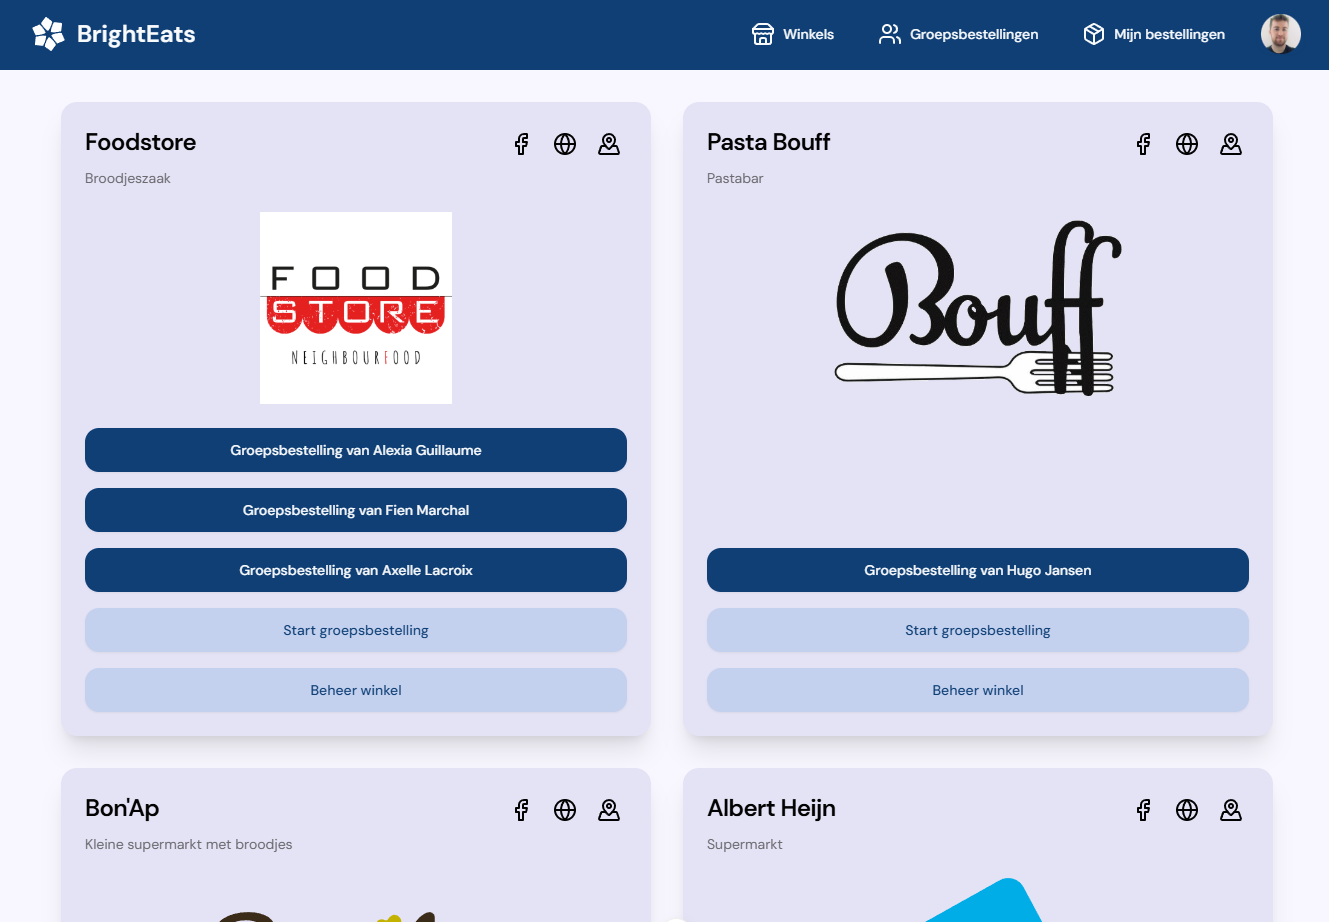
\includegraphics[width=0.8\textwidth]{brighteats.png}
    \caption{De homepage van de BrightEats applicatie.}
    \label{fig:brighteats}
\end{figure}

\begin{figure}[H]
    \centering
    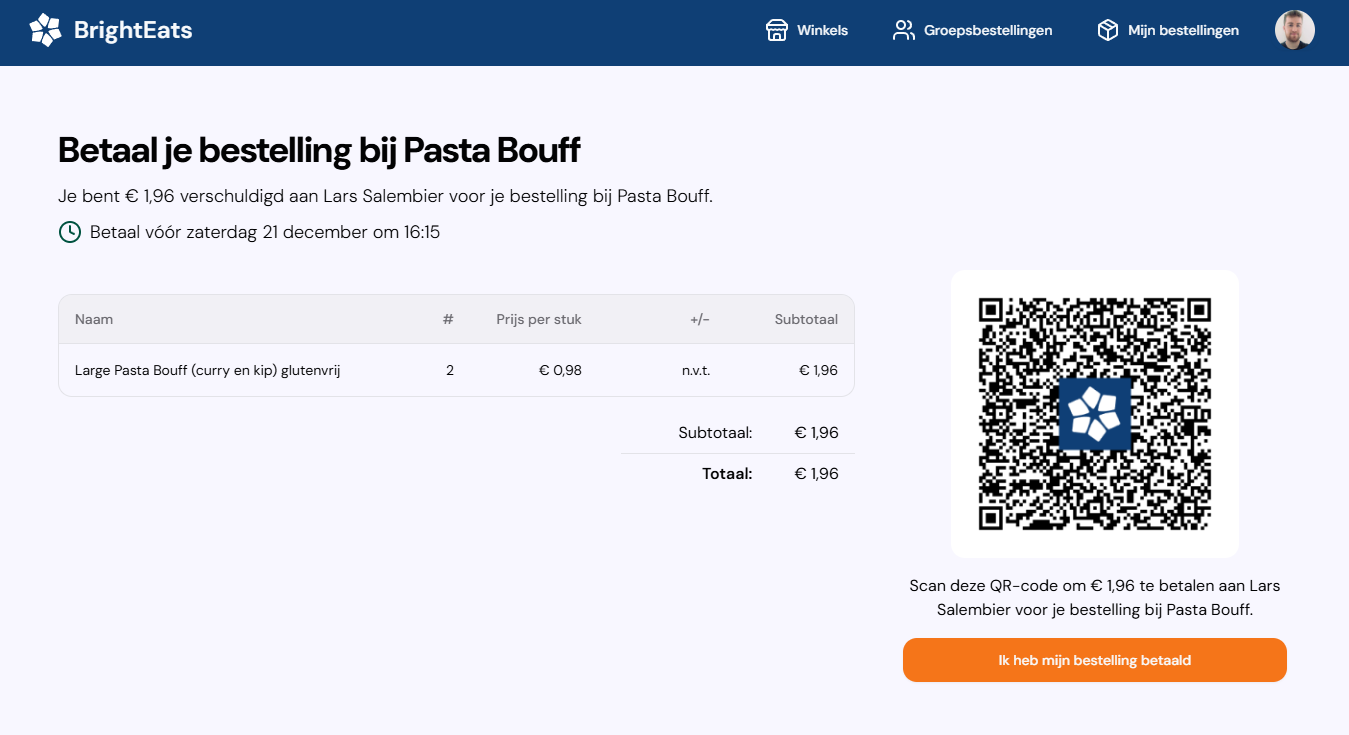
\includegraphics[width=0.8\textwidth]{brighteats-payment-page.png}
    \caption{De betalingspagina van de BrightEats applicatie, met een QR-code voor de betaling.}
    \label{fig:brighteats-shop}
\end{figure}

\bigskip

Authenticatie gebeurt via Google SSO, waarbij gebruikers inloggen met hun BrightAnalytics Google account. De backend API is verantwoordelijk voor het beheren van gebruikers, winkels, menu's, groepsbestellingen en betalingsverzoeken. De frontend applicatie is verantwoordelijk voor het tonen van deze gegevens en het toelaten van interactie met de gebruiker.

\section{Backend - Algemene aanpak}

De implementatie van de RESTful principes in de Laravel backend van de BrightEats API werd aangepakt met een iteratieve aanpak, waarbij we stapsgewijs verschillende onderdelen van de API ontwikkelden en verfijnden. Hierbij maakten we veel gebruik van Laravel's ingebouwde functionaliteiten, zoals resource controllers en routes, en hielden we ons zo veel mogelijk aan de opgestelde richtlijnen.

\subsection{Architectuur en RESTful principes}

Laravel's architectuur is perfect voor het bouwen van RESTful API's. We maken gebruik van resource controllers om gestructureerd CRUD-operaties (Create, Read, Update, Delete) op onze resources, zoals \texttt{Order}, \texttt{Shop}, \texttt{Item} en \texttt{GroupOrder}, te definiëren. Deze controllers worden gekoppeld aan routes in het \texttt{api.php} bestand, dat dient als het centrale punt voor het definiëren van alle API endpoints.

\subsubsection{Autorisatie}

Voor autorisatie gebruiken we Policies. Zo is er bijvoorbeeld een \texttt{OrderPolicy} die bepaalt welke gebruikers welke acties mogen uitvoeren op een \texttt{Order}.

\subsubsection{Validatie}

Voor validatie gebruiken we specifieke request classes, zoals \texttt{StoreOrderRequest} en \texttt{UpdateOrderRequest}, die de validatieregels voor inkomende requests definiëren.

\subsubsection{Authenticatie}

Authenticatie wordt afgehandeld door Laravel Sanctum. Dit pakket biedt een eenvoudige manier om API tokens te beheren en gebruikers te authenticeren. Voor BrightEats is Google Single Sign-On (SSO) de enige authenticatiemethode. Gebruikers loggen in door een POST request te sturen naar \texttt{/users} met hun Google credential. Het systeem verifieert deze credential en genereert een Sanctum token voor de gebruiker.

\subsubsection{Businesslogica}

De businesslogica bevindt zich voornamelijk in Service classes. Voor orders hebben we bijvoorbeeld de \texttt{OrderService}, \texttt{OrderItemsManager} en \texttt{QrCodeGenerator} classes, die verantwoordelijk zijn voor respectievelijk het beheren van orders, het beheren van order items en het genereren van QR-codes voor betalingen. Models, zoals \texttt{Order}, bevatten eenvoudige berekeningen en methoden, terwijl complexere logica wordt geabstraheerd naar services.

\subsubsection{Datarepresentatie}

Voor het terugsturen van data gebruiken we API Resources. Deze transformeren de models naar een JSON-structuur die geschikt is voor de API. We gebruiken verschillende resources, zoals \texttt{OrderResource}, \texttt{OrderResourceWithItems} en \texttt{OrderResourceWithGroupOrder}, om de nodige data te embedden, afhankelijk van de context.

\section{Beschrijving van de API Routes}

Het \texttt{api.php} bestand definieert alle routes voor de BrightEats API. Hieronder volgt een gedetailleerde beschrijving van elke route, gegroepeerd per resource en functionaliteit. Alle routes, met uitzondering van de inlog-route, vallen onder de \texttt{auth:sanctum} middleware, wat betekent dat gebruikers geauthenticeerd moeten zijn om toegang te krijgen.

\subsection{Authenticatie}

\begin{itemize}
  \item \textbf{POST /users:} Deze route wordt gebruikt voor authenticatie via Google SSO. Gebruikers sturen hun Google credential mee in de request body. Deze credential wordt door de Google API in de frontend ontvangen. Bij succesvolle validatie wordt een Sanctum token gegenereerd en teruggestuurd. Dit is de enige manier om in te loggen in de applicatie.
\end{itemize}

\subsection{Winkels (shops)}

\begin{itemize}
  \item \textbf{GET /shops:} Haalt een lijst op van alle winkels. Dit endpoint geeft per winkel ook alle groepsbestellingen terug die momenteel openstaan.
  \item \textbf{POST /shops:} Maakt een nieuwe winkel aan.
  \item \textbf{GET /shops/{shop}:} Haalt de details van een specifieke winkel op, geïdentificeerd door \texttt{{shop}}.
  \item \textbf{PATCH /shops/{shop}:} Werkt de gegevens van een specifieke winkel bij.
  \item \textbf{DELETE /shops/{shop}:} Verwijdert een specifieke winkel.
  \item \textbf{POST /shops/{shop}/group-orders:} Maakt een nieuwe groepsbestelling aan bij een specifieke winkel.
\end{itemize}

\subsection{Items (binnen een winkel)}

\begin{itemize}
  \item \textbf{POST /shops/{shop}/items:} Maakt een nieuw item aan in de catalogus van een specifieke winkel.
  \item \textbf{GET /shops/{shop}/items:} Haalt een lijst op van alle items in de catalogus van een specifieke winkel.
  \item \textbf{GET /shops/{shop}/items/{item}:} Haalt de details van een specifiek item op, geïdentificeerd door \texttt{{item}}, binnen de catalogus van een specifieke winkel.
  \item \textbf{PATCH /shops/{shop}/items/{item}:} Werkt de gegevens van een specifiek item bij.
  \item \textbf{DELETE /shops/{shop}/items/{item}:} Verwijdert een specifiek item uit de catalogus van een winkel.
\end{itemize}

\subsection{Groepsbestellingen (Group Orders)}

\begin{itemize}
  \item \textbf{GET /group-orders:} Haalt een lijst op van alle groepsbestellingen waarvan de ingelogde gebruiker deel uitmaakt.
  \item \textbf{GET /group-orders/{groupOrder}:} Haalt de details van een specifieke groepsbestelling op.
  \item \textbf{PATCH /group-orders/{groupOrder}:} Werkt de gegevens van een specifieke groepsbestelling bij.
  \item \textbf{DELETE /group-orders/{groupOrder}:} Verwijdert een specifieke groepsbestelling.
\end{itemize}

\subsection{Bestellingen (binnen een Groepsbestelling)}

\begin{itemize}
  \item \textbf{POST /group-orders/{groupOrder}/orders:} Maakt een nieuwe bestelling aan binnen een specifieke groepsbestelling.
  \item \textbf{GET /group-orders/{groupOrder}/orders:} Haalt een lijst op van alle bestellingen binnen een specifieke groepsbestelling. De bestellingen bevatten ook hun items en de gebruiker die de bestelling heeft geplaatst.
\end{itemize}

\subsection{Bestellingen (Orders)}

\begin{itemize}
  \item \textbf{GET /orders:} Haalt een lijst op van alle bestellingen van de ingelogde gebruiker. Deze route is gepagineerd.
  \item \textbf{GET /orders/{order}:} Haalt de details van een specifieke bestelling op.
  \item \textbf{PATCH /orders/{order}:} Werkt de gegevens van een specifieke bestelling bij.
  \item \textbf{DELETE /orders/{order}:} Verwijdert een specifieke bestelling.
  \item \textbf{GET /orders/{order}/payment-qr-code:} Genereert een QR-code voor de betaling van een specifieke bestelling.
\end{itemize}

\subsection{Gebruikers (Users)}

\begin{itemize}
\item \textbf{GET /users:} Haalt een lijst van alle gebruikers op (beperkt tot admins).
\item \textbf{GET /users/me:} Haalt de gegevens van de ingelogde gebruiker op.
\item \textbf{GET /users/{user}:} Haalt de gegevens van een specifieke gebruiker op.
\item \textbf{PATCH /users/{user}:} Werkt de gegevens van een specifieke gebruiker bij.
\end{itemize}

\begin{minted}{php}
<?php

declare(strict_types=1);

// (imports weggelaten)

Route::post('/users', [UserController::class, 'store'])->name('users.store');

Route::middleware('auth:sanctum')->group(function () {
  Route::prefix('shops')
  ->name('shops.')
  ->group(function () {
    Route::get('/', [ShopController::class, 'index'])->name('index');
    Route::post('/', [ShopController::class, 'store'])->name('store');
    Route::get('/{shop}', [ShopController::class, 'show'])->name('show');
    Route::patch('/{shop}', [ShopController::class, 'update'])->name('update');
    Route::delete('/{shop}', [ShopController::class, 'delete'])->name('delete');
    Route::post('/{shop}/group-orders', [GroupOrderController::class, 'store'])->name('group-orders.store');
    Route::prefix('/{shop}/items')
      ->name('items.')
      ->group(function () {
        Route::post('/', [ItemController::class, 'store'])->name('store');
        Route::get('/', [ItemController::class, 'index'])->name('index');
        Route::get('/{item}', [ItemController::class, 'show'])->name('show');
        Route::patch('/{item}', [ItemController::class, 'update'])->name('update');
        Route::delete('/{item}', [ItemController::class, 'delete'])->name('delete');
  });
});

Route::prefix('/group-orders')
  ->name('group-orders.')
  ->group(function () {
    Route::get('/', [GroupOrderController::class, 'index'])->name('index');
    Route::get('/{groupOrder}', [GroupOrderController::class, 'show'])->name('show');
    Route::patch('/{groupOrder}', [GroupOrderController::class, 'update'])->name('update');
    Route::delete('/{groupOrder}', [GroupOrderController::class, 'delete'])->name('delete');
    Route::prefix('{groupOrder}/orders')
      ->name('orders.')
      ->group(function () {
      Route::post('/', [OrderController::class, 'store'])->name('store');
      Route::get('/', [OrderController::class, 'getOrdersInGroupOrder'])->name('index');
    });
});

Route::prefix('/orders')
  ->name('orders.')
  ->group(function () {
    Route::get('/', [OrderController::class, 'index'])->name('index');
    Route::get('/{order}', [OrderController::class, 'show'])->name('show');
    Route::patch('/{order}', [OrderController::class, 'update'])->name('update');
    Route::delete('/{order}', [OrderController::class, 'delete'])->name('delete');
    Route::get('/{order}/payment-qr-code', [OrderController::class, 'generatePaymentQrCode'])->name('payment-qr-code');
});

Route::prefix('/users')
  ->name('users.')
  ->group(function () {
    Route::get('/', [UserController::class, 'index'])->name('index');
    Route::get('/me', [UserController::class, 'me'])->name('me');
    Route::get('/{user}', [UserController::class, 'show'])->name('show');
    Route::patch('/{user}', [UserController::class, 'update'])->name('update');
  });
});
\end{minted}
\label{lst:api_routes}

\section{Conclusie}

De implementatie van de BrightEats API volgt een gestructureerde aanpak, waarbij Laravel's functionaliteiten optimaal worden benut om een RESTful architectuur te realiseren. Door gebruik te maken van resource controllers, routes, policies, request classes, response classes, models en service classes, is een robuuste en schaalbare API gecreëerd.

\section{Case study: \texttt{GroupOrder} Resource}

Elke route volledig bespreken zou te ver gaan voor dit hoofdstuk. Daarom zullen we ons beperken tot een case study van de \texttt{GroupOrder} resource. We analyseren de code van de \texttt{GroupOrderController}, de \texttt{GroupOrderService}, het \texttt{GroupOrder} model, de gebruikte API resources, de request classes en de policies die de autorisatie regelen.

\subsection{De \texttt{GroupOrderController}}

De \texttt{GroupOrderController} is verantwoordelijk voor het afhandelen van HTTP requests gerelateerd aan groepsbestellingen. Deze controller is opgezet volgens de principes van resource controllers in Laravel en maakt gebruik van dependency injection om de \texttt{GroupOrderService} te injecteren.

\begin{minted}{php}
  <?php

  declare(strict_types=1);
  
  namespace App\Http\Controllers;
  
  // (imports weggelaten)
  
  class GroupOrderController extends Controller
  {
      public function __construct(private readonly GroupOrderService $groupOrderService) {}
  
      public function index(Request $request): AnonymousResourceCollection
      {
          $this->authorize('index', GroupOrder::class);
  
          /** @var User $user */
          $user = $request->user();
  
          $groupOrders = $this->groupOrderService->getGroupOrdersForCoordinator($user);
  
          return GroupOrderResourceWithShop::collection($groupOrders);
      }
  
      public function store(StoreGroupOrderRequest $request, Shop $shop): JsonResponse
      {
          $this->authorize('store', [GroupOrder::class, $shop]);
  
          /** @var User $user */
          $user = $request->user();
  
          /** @var array{
           *     order_deadline: string,
           *     payment_deadline: string,
           *     notes?: string|null,
           *     is_delivery?: bool|null,
           *     payment_system_enabled?: bool|null,
           * } $validatedData
           */
          $validatedData = $request->validated();
  
          $groupOrder = $this->groupOrderService->createGroupOrder($validatedData, $shop, $user->id);
  
          $groupOrder = $groupOrder->refresh();
  
          return response()->json(new GroupOrderResource($groupOrder), ResponseAlias::HTTP_CREATED, [
              'Location' => route('group-orders.show', [$groupOrder->id]),
          ]);
      }
  
      public function show(GroupOrder $groupOrder): JsonResponse
      {
          $this->authorize('show', $groupOrder);
  
          return response()->json(new GroupOrderResourceWithCoordinatorAndShopAndOrders($groupOrder));
      }
  
      public function update(UpdateGroupOrderRequest $request, GroupOrder $groupOrder): JsonResponse
      {
          /**
           * @var array{
           *     order_deadline?: string|null,
           *     payment_deadline?: string|null,
           *     notes?: string|null,
           *     is_delivery?: bool|null,
           *     cost_difference?: array{amount_in_cents?: int|null, reason?: string|null}|null,
           *     payment_system_enabled?: bool|null,
           * } $validatedData
           */
          $validatedData = $request->validated();
  
          $this->authorize('update', [$groupOrder, $validatedData]);
  
          $this->groupOrderService->updateGroupOrder($groupOrder, $validatedData);
  
          return response()->json(new GroupOrderResource($groupOrder));
      }
  
      public function delete(GroupOrder $groupOrder): Response
      {
          $this->authorize('delete', $groupOrder);
  
          $this->groupOrderService->removeGroupOrder($groupOrder);
  
          return response()->noContent();
      }
  }
\end{minted}
\label{lst:groupordercontroller_class}

De controller bevat de volgende methoden, die overeenkomen met de standaard RESTful acties:

\begin{itemize}
  \item \texttt{index(Request \$request)}: Deze methode haalt een lijst op van alle GroupOrders die gecoördineerd worden door de ingelogde gebruiker. De \texttt{GroupOrderPolicy} autoriseert de actie. De \texttt{GroupOrderService} haalt de data op en de \texttt{GroupOrderResourceWithShop} resource formatteert de response. De methode accepteert een GET request naar de \texttt{/group-orders} route.
  \item \texttt{store(StoreGroupOrderRequest \$request, Shop \$shop)}: Deze methode maakt een nieuwe \texttt{GroupOrder} aan. De \texttt{StoreGroupOrderRequest} valideert de request data en de \texttt{GroupOrderPolicy} autoriseert de actie. De \texttt{GroupOrderService} creëert de \texttt{GroupOrder} en een \texttt{GroupOrderResource} formatteert de response, inclusief een \texttt{Location} header naar de aangemaakte resource. De methode accepteert een POST request naar de \texttt{/shops/\{shop\}/group-orders} route.
  \item \texttt{show(GroupOrder \$groupOrder)}: Deze methode haalt de details van een specifieke \texttt{GroupOrder} op. De \texttt{GroupOrderPolicy} autoriseert de actie op basis van de status van de \texttt{GroupOrder} en de relatie van de gebruiker tot de \texttt{GroupOrder}. De \texttt{GroupOrderResourceWithCoordinatorAndShopAndOrders} resource formatteert de response. De methode accepteert een GET request naar de \texttt{/group-orders/\{groupOrder\}} route.
  \item \texttt{update(UpdateGroupOrderRequest \$request, GroupOrder \$groupOrder)}: Deze methode werkt een bestaande \texttt{GroupOrder} bij. De \texttt{UpdateGroupOrderRequest} valideert de request data en de \texttt{GroupOrderPolicy} autoriseert de actie. De \texttt{GroupOrderService} werkt de \texttt{GroupOrder} bij en een \texttt{GroupOrderResource} formatteert de response. De methode accepteert een PATCH request naar de \texttt{/group-orders/\{groupOrder\}} route.
  \item \texttt{delete(GroupOrder \$groupOrder)}: Deze methode verwijdert of annuleert een \texttt{GroupOrder}. De \texttt{GroupOrderPolicy} autoriseert de actie. De \texttt{GroupOrderService} verwijdert of annuleert de \texttt{GroupOrder}, afhankelijk van of er al bestellingen geplaatst zijn. Er wordt een 204 No Content response teruggestuurd. De methode accepteert een DELETE request naar de \texttt{/group-orders/\{groupOrder\}} route.
\end{itemize}

Hieronder is een codevoorbeeld van de \texttt{GroupOrderController}, met de implementatie van de index, show en store methoden.

\subsection{De \texttt{GroupOrderService} en het \texttt{GroupOrder} Model}

De \texttt{GroupOrderService} bevat de business logica voor het beheren van \texttt{GroupOrders}. Deze service wordt geïnjecteerd in de \texttt{GroupOrderController} en voert acties uit zoals het ophalen, aanmaken, bijwerken en verwijderen van GroupOrders. Het \texttt{GroupOrder} model vertegenwoordigt een groepsbestelling in de database en definieert relaties met andere modellen, zoals Shop en User (via de coordinator\_id). Het model bevat ook methoden voor het berekenen van totalen, statussen en het valideren van data.

\begin{minted}{php}
    <?php

    declare(strict_types=1);
    
    namespace App\Services;
    
    // (imports weggelaten)
    
    class GroupOrderService
    {
        public function getGroupOrdersForCoordinator(User $coordinator): Collection
        {
            return GroupOrder::with('shop')->where('coordinator_id', $coordinator->id)->get();
        }
    
        public function createGroupOrder(array $data, Shop $shop, int $userId): GroupOrder
        {
            return $shop->groupOrders()->create([
                'order_deadline' => $data['order_deadline'],
                'payment_deadline' => $data['payment_deadline'],
                'notes' => $data['notes'] ?? null,
                'is_delivery' => $data['is_delivery'] ?? false,
                'payment_system_enabled' => $data['payment_system_enabled'] ?? true,
                'coordinator_id' => $userId,
            ]);
        }
    
        public function updateGroupOrder(GroupOrder $groupOrder, array $data): void
        {
            $costDifference = $this->processCostDifference($data);
    
            foreach (['order_deadline', 'payment_deadline', 'is_delivery', 'payment_system_enabled'] as $key) {
                if (! isset($data[$key])) {
                    /** @noinspection PhpConditionAlreadyCheckedInspection - this is a false positive. If the key is null, we want to unset it. */
                    unset($data[$key]);
                }
            }
    
            $groupOrder->update(array_merge($data, $costDifference));
        }
    
        private function processCostDifference(array $data): array
        {
            $result = [
                'cost_difference_in_cents' => 0,
                'cost_difference_reason' => null,
            ];
    
            $costDifference = $data['cost_difference'] ?? null;
            if ($costDifference) {
                $result['cost_difference_reason'] = $costDifference['reason'] ?? null;
                $result['cost_difference_in_cents'] = $costDifference['amount_in_cents'] ?? 0;
    
                if (($costDifference['amount_in_cents'] ?? 0) === 0) {
                    $result['cost_difference_reason'] = null;
                }
            }
    
            return $result;
        }
    
        public function removeGroupOrder(GroupOrder $groupOrder): void
        {
            if ($groupOrder->orders()->where('user_id', '!=', $groupOrder->coordinator_id)->exists()) {
                $groupOrder->update(['status' => GroupOrderStatus::CANCELLED]);
            } else {
                $groupOrder->delete();
            }
        }
    }
\end{minted}
\label{lst:grouporderservice}

\begin{minted}{php}
  <?php

  declare(strict_types=1);
  
  namespace App\Models;
  
  // (imports weggelaten)
  
  /**
   * @property int $id
   * @property int $shop_id
   * @property int $coordinator_id
   * @property Carbon $order_deadline
   * @property Carbon $payment_deadline
   * @property string|null $notes
   * @property bool $is_delivery
   * @property GroupOrderStatus $status
   * @property int $cost_difference_in_cents
   * @property string|null $cost_difference_reason
   * @property bool $payment_system_enabled
   * @property Carbon $created_at
   * @property Carbon|null $updated_at
   * @property-read User $coordinator
   * @property-read Collection<int, Order> $orders
   * @property-read Shop $shop
   */
  class GroupOrder extends Model
  {
      use HasFactory;
  
      public const int NOTES_MAX_LENGTH = 255;
  
      public const int COST_DIFFERENCE_REASON_MAX_LENGTH = 255;
  
      public const int COST_DIFFERENCE_IN_CENTS_MIN = -100000;
  
      public const int COST_DIFFERENCE_IN_CENTS_MAX = 100000;
  
      protected $fillable = [
          'shop_id',
          'coordinator_id',
          'order_deadline',
          'payment_deadline',
          'notes',
          'is_delivery',
          'status',
          'cost_difference_in_cents',
          'cost_difference_reason',
          'payment_system_enabled',
      ];
  
      protected $casts = [
          'order_deadline' => 'datetime',
          'payment_deadline' => 'datetime',
          'is_delivery' => 'boolean',
          'status' => GroupOrderStatus::class,
          'cost_difference_in_cents' => 'integer',
          'payment_system_enabled' => 'boolean',
      ];
  
      protected $attributes = [
          'is_delivery' => false,
          'status' => GroupOrderStatus::OPEN,
          'cost_difference_in_cents' => 0,
          'payment_system_enabled' => true,
      ];
  
      public function shop(): BelongsTo
      {
          return $this->belongsTo(Shop::class);
      }
  
      public function coordinator(): BelongsTo
      {
          return $this->belongsTo(User::class, 'coordinator_id');
      }
  
      public function totalPriceInCents(): int
      {
          return intval($this->orders->sum(fn (Order $order) => $order->totalPriceInCents()));
      }
  
      public function isCoordinator(int $userId): bool
      {
          return $this->coordinator_id === $userId;
      }
  
      public function isParticipant(int $userId): bool
      {
          return $this->orders()->where('user_id', $userId)->exists();
      }
  
      public function orders(): HasMany
      {
          return $this->hasMany(Order::class);
      }
  
      public function hasBeenCancelled(): bool
      {
          return $this->status === GroupOrderStatus::CANCELLED;
      }
  
      public function hasAnyOrdersWherePaymentProcessStarted(): bool
      {
          return $this->orders()
              ->where(function ($query) {
                  $query->where('user_indicated_payment', true)
                      ->orWhere('payment_confirmed', true);
              })
              ->exists();
      }
  
      public function getSplitCostDifference(): int
      {
          if (! $this->getNonemptyOrdersCount()) {
              return 0;
          }
  
          return intval(ceil($this->cost_difference_in_cents / $this->getNonemptyOrdersCount()));
      }
  
      public function getNonemptyOrdersCount(): int
      {
          return $this->orders()->whereHas('items', function ($query) {
              $query->where('available', true)->where(function ($query) {
                  $query->where('price_on_purchase_in_cents', '>', 0)
                      ->orWhere('cost_difference_in_cents', '>', 0);
              });
          })->count();
      }
  
      public function getDerivedStatus(): GroupOrderStatus
      {
          if ($this->status === GroupOrderStatus::CANCELLED) {
              return GroupOrderStatus::CANCELLED;
          }
  
          if ($this->orders()->count() === 0 && ! $this->orderDeadlineHasPassed()) {
              return GroupOrderStatus::OPEN;
          }
  
          if ($this->hasBeenFullyConfirmedPaid()) {
              return GroupOrderStatus::FULLY_CONFIRMED_PAID;
          }
  
          if ($this->hasBeenFullyPaid()) {
              return GroupOrderStatus::FULLY_PAID;
          }
  
          $nonEmptyOrders = $this->getNonEmptyOrders();
  
          if ($nonEmptyOrders->some(fn ($order) => $order->user_indicated_payment || $order->payment_confirmed)) {
              return GroupOrderStatus::PARTIALLY_PAID;
          }
  
          if ($nonEmptyOrders->every(fn ($order) => $order->payment_is_allowed)) {
              return GroupOrderStatus::PAYMENT_POSSIBLE;
          }
  
          if ($this->orderDeadlineHasPassed()) {
              return GroupOrderStatus::CLOSED;
          }
  
          return GroupOrderStatus::OPEN;
      }
  
      public function orderDeadlineHasPassed(): bool
      {
          return $this->order_deadline < now();
      }
  
      private function hasBeenFullyConfirmedPaid(): bool
      {
          return $this->orders()->where('payment_confirmed', true)->count() >= $this->getNonemptyOrdersCount();
      }
  
      private function hasBeenFullyPaid(): bool
      {
          return $this->orders()->where('user_indicated_payment', true)->count() >= $this->getNonemptyOrdersCount();
      }
  
      private function getNonEmptyOrders(): Collection
      {
          return $this->orders()->whereHas('items', function ($query) {
              $query->where('available', true);
          })->get();
      }
  
      public function isStillActive(): bool
      {
          $twoDaysAgo = Carbon::now()->subDays(2);
  
          if ($this->order_deadline > $twoDaysAgo) {
              return true;
          }
  
          if ($this->status === GroupOrderStatus::CANCELLED && $this->updated_at > $twoDaysAgo) {
              return true;
          }
  
          if (! $this->payment_system_enabled) {
              return false;
          }
  
          return $this->orders()->where('payment_confirmed', true)->count() < $this->getNonemptyOrdersCount();
      }
  }
\end{minted}
\label{lst:groupordermodel}

\subsection{API Resources}

Voor het formatteren van de responses wordt gebruik gemaakt van API Resources. Deze transformeren de \texttt{GroupOrder} objecten naar een gestructureerd JSON formaat. Er zijn verschillende resources gedefinieerd voor \texttt{GroupOrders}, afhankelijk van de context en de benodigde data:

\begin{itemize}
\item \texttt{GroupOrderResource}: De basisresource voor een \texttt{GroupOrder}, met basisinformatie zoals \texttt{id}, \texttt{order\_deadline}, \texttt{payment\_deadline}, \texttt{notes}, \texttt{is\_delivery}, \texttt{orders\_count}, \texttt{cost\_difference}, \texttt{status}, \texttt{total\_in\_cents} en \texttt{payment\_system\_enabled}.
\item \texttt{GroupOrderResourceWithShop}: Breidt \texttt{GroupOrderResource} uit met informatie over de bijhorende \texttt{Shop}. Wordt gebruikt in de \texttt{index} methode van de \texttt{GroupOrderController}.
\item \texttt{GroupOrderResourceWithCoordinatorAndShopAndOrders}: Breidt \texttt{GroupOrderResource} uit met informatie over de coördinator (\texttt{User}), de bijhorende \texttt{Shop} en alle \texttt{Orders} in de \texttt{GroupOrder}. Wordt gebruikt in de \texttt{show} methode van de \texttt{GroupOrderController}.
\end{itemize}

Hieronder wordt de basis \texttt{GroupOrderResource} getoond. De andere resources extenden deze basisresource en voegen extra data toe.

\begin{minted}{php}
  <?php

  declare(strict_types=1);
  
  namespace App\Http\Resources\GroupOrder;
  
  // (imports weggelaten)	
  
  class GroupOrderResource extends JsonResource
  {
      public function toArray(Request $request): array
      {
          return [
              'id' => $this->id,
              'order_deadline' => $this->order_deadline,
              'payment_deadline' => $this->payment_deadline,
              'notes' => $this->notes,
              'is_delivery' => $this->is_delivery,
              'orders_count' => $this->getNonemptyOrdersCount(),
              'cost_difference' => [
                  'amount_in_cents' => $this->cost_difference_in_cents,
                  'reason' => $this->cost_difference_reason,
                  'amount_per_order_in_cents' => $this->getSplitCostDifference(),
              ],
              'status' => $this->getDerivedStatus(),
              'total_in_cents' => $this->totalPriceInCents(),
              'payment_system_enabled' => $this->payment_system_enabled,
          ];
      }
  }
\end{minted}
\label{lst:grouporderresource}

\subsection{Requests}

Voor het valideren van de inkomende request data bij het aanmaken en bijwerken van \texttt{GroupOrders} worden specifieke form request classes gebruikt. Deze classes, \texttt{StoreGroupOrderRequest} en \texttt{UpdateGroupOrderRequest}, definiëren de validatieregels voor de velden die in de request body mogen voorkomen.

\bigskip

Omdat de API zowel Nederlandse als Engelse foutmeldingen ondersteunt, worden de validatieregels en foutmeldingen in aparte bestanden gedefinieerd. De Laravel-functie \texttt{\_\_()} wordt gebruikt om de localization strings op te halen.

\bigskip

Bij requests werd steeds de Wet van Postel gevolgd: wees conservatief in wat je stuurt, en liberaal in wat je accepteert. Dit betekent dat de API zo tolerant mogelijk is voor de input van de gebruiker, maar dat de output zo correct mogelijk is. Zo zie je bijvoorbeeld dat \texttt{notes} zowel \texttt{nullable} als \texttt{sometimes} is. Hierdoor zullen lege strings, null-waarden en ontbrekende velden allemaal geaccepteerd worden. Voor de boolean-velden \texttt{is\_delivery} en \texttt{payment\_system\_enabled} geldt ook dat deze niet noodzakelijk moeten worden meegegeven en dat ze standaard op \texttt{false} en \texttt{true} worden gezet. Op die manier kan de gebruiker deze velden weglaten als ze de standaardwaarde willen gebruiken. Bovendien is deze manier van werken erg handig om backwards compatibiliteit te garanderen bij het toevoegen van nieuwe velden aan de request.

\begin{minted}{php}
  <?php

declare(strict_types=1);

namespace App\Http\Requests\GroupOrder;

use App\Models\GroupOrder;
use Illuminate\Foundation\Http\FormRequest;

class StoreGroupOrderRequest extends FormRequest
{
    public function rules(): array
    {
        return [
            'order_deadline' => 'required|date|after:now',
            'payment_deadline' => 'required|date|after:now|after_or_equal:order_deadline',
            'notes' => 'sometimes|nullable|string|max:'.GroupOrder::NOTES_MAX_LENGTH,
            'is_delivery' => 'sometimes|nullable|boolean',
            'payment_system_enabled' => 'sometimes|nullable|boolean',
        ];
    }

    public function messages(): array
    {
        return [
            'order_deadline.required' => __('validation.group_order.order_deadline.required'),
            'order_deadline.date' => __('validation.group_order.order_deadline.date'),
            'order_deadline.after' => __('validation.group_order.order_deadline.after'),
            'payment_deadline.required' => __('validation.group_order.payment_deadline.required'),
            'payment_deadline.date' => __('validation.group_order.payment_deadline.date'),
            'payment_deadline.after' => __('validation.group_order.payment_deadline.after'),
            'payment_deadline.after_or_equal' => __('validation.group_order.payment_deadline.after_or_equal_order_deadline'),
            'notes.string' => __('validation.group_order.notes.string'),
            'notes.max' => __('validation.group_order.notes.max', ['max' => GroupOrder::NOTES_MAX_LENGTH]),
            'is_delivery.boolean' => __('validation.group_order.is_delivery.boolean'),
            'payment_system_enabled.boolean' => __('validation.group_order.payment_system_enabled.boolean'),
        ];
    }
}

\end{minted}
\label{lst:storegrouporderrequest}

\subsection{Policies}

De autorisatie van acties wordt afgehandeld door policies. Policies definiëren de authorisatielogica voor een bepaald model. In dit geval is er een \texttt{GroupOrderPolicy} die de autorisatieregels voor \texttt{GroupOrders} bevat. De policy bevat methoden voor elke actie die geautoriseerd moet worden, zoals \texttt{index}, \texttt{store}, \texttt{show}, \texttt{update} en \texttt{delete}.

\begin{minted}{php}
  <?php

  declare(strict_types=1);
  
  namespace App\Policies;
  
  // (imports weggelaten)
  
  class GroupOrderPolicy
  {
      use HandlesAuthorization;
  
      public function index(): Response
      {
          return Response::allow();
      }
  
      public function store(User $user, Shop $shop): Response
      {
          if (! $shop->is_active) {
              return Response::deny(__('authorization.group_order.store.shop_not_active'));
          }
  
          if ($user->iban === null) {
              return Response::deny(__('authorization.group_order.store.no_iban'));
          }
  
          return Response::allow();
      }
  
      public function show(User $user, GroupOrder $groupOrder): Response
      {
          if ($groupOrder->hasBeenCancelled() && ! $groupOrder->isCoordinator($user->id) && ! $groupOrder->isParticipant($user->id)) {
              return Response::deny(__('authorization.group_order.show.cancelled'));
          }
  
          if ($groupOrder->orderDeadlineHasPassed() && ! $groupOrder->isCoordinator($user->id) && ! $groupOrder->isParticipant($user->id)) {
              return Response::deny(__('authorization.group_order.show.deadline_passed'));
          }
  
          return Response::allow();
      }
  
      public function update(User $user, GroupOrder $groupOrder, array $data): Response
      {
          if ($groupOrder->hasBeenCancelled()) {
              return Response::deny(__('authorization.group_order.update.cancelled'));
          }
  
          if (! $groupOrder->isCoordinator($user->id)) {
              return Response::deny(__('authorization.group_order.update.not_coordinator'));
          }
  
          // You can only update `cost_difference` if the deadline has passed.
          if (isset($data['cost_difference']['amount_in_cents'])
              && $data['cost_difference']['amount_in_cents'] !== $groupOrder->cost_difference_in_cents) {
              if (! $groupOrder->orderDeadlineHasPassed()) {
                  return Response::deny(__('authorization.group_order.update.cost_difference.deadline_not_passed'));
              }
  
              // additionally, no payment process should have started yet
              if ($groupOrder->hasAnyOrdersWherePaymentProcessStarted()) {
                  return Response::deny(__('authorization.group_order.update.cost_difference.payment_process_started'));
              }
          }
  
          return Response::allow();
      }
  
      public function delete(User $user, GroupOrder $groupOrder): Response
      {
          if (! $groupOrder->isCoordinator($user->id)) {
              return Response::deny(__('authorization.group_order.delete.not_coordinator'));
          }
  
          if ($groupOrder->hasAnyOrdersWherePaymentProcessStarted()) {
              return Response::deny(__('authorization.group_order.delete.payment_process_started'));
          }
  
          return Response::allow();
      }
  }
\end{minted}
\label{lst:grouporderpolicy}

\subsection{Conclusie}

De case study van de \texttt{GroupOrder} resource illustreert hoe de verschillende onderdelen van de BrightEats API samenwerken om een RESTful API te realiseren. De \texttt{GroupOrderController} handelt de HTTP requests af, de \texttt{GroupOrderService} bevat de business logica, het \texttt{GroupOrder} model vertegenwoordigt de data in de database, de API resources formatteren de responses, de request classes valideren de request data en de policies autoriseren de acties. Door deze onderdelen op een gestructureerde manier te implementeren, wordt een robuuste en schaalbare API gecreëerd.

\section{Frontend - Algemene Aanpak}

De Vue.js frontend van de BrightEats applicatie communiceert met de RESTful API via HTTP requests. Voor het uitvoeren van deze requests wordt gebruik gemaakt van de Axios library. Axios biedt een gebruiksvriendelijke interface voor het maken van HTTP requests en het verwerken van responses.

\subsection{Axios Configuratie}

Het \texttt{utils/api.ts} bestand bevat de basisconfiguratie voor Axios. Hier wordt een Axios instantie gecreëerd met de basis URL van de API en standaard headers voor \texttt{Content-Type} en \texttt{Accept}.

\begin{minted}{typescript}
import axios, { HttpStatusCode, isAxiosError } from 'axios'
import { getAccessToken } from '@/services/tokenService'
import router, { RouteNames } from '@/router'
import { defaultLanguage, LOCALE_LOCAL_STORAGE_KEY } from '@/config/i18n'

const API_URL = import.meta.env.VITE_API_URL

const api = axios.create({
    baseURL: API_URL,
    headers: {
        'Content-Type': 'application/json',
        Accept: 'application/json'
    }
})

api.interceptors.request.use(
    (config) => {
        const accessToken = getAccessToken()
        if (accessToken) {
            config.headers['Authorization'] = `Bearer ${accessToken}`
        }
        config.headers['Accept-Language'] =
            localStorage.getItem(LOCALE_LOCAL_STORAGE_KEY) || defaultLanguage.code
        return config
    },
    (error) => Promise.reject(error)
)

api.interceptors.response.use(
    (response) => response,
    async (error) => {
        const originalRequest = error.config

        if (error.status === HttpStatusCode.Unauthorized && !originalRequest._retry) {
            originalRequest._retry = true
            await router.push({ name: RouteNames.LoginSignup })
        }

        return Promise.reject(error)
    }
)

export default api

function isAxiosErrorWithStatus(error: unknown, status: HttpStatusCode): boolean {
    return isAxiosError(error) && error.response?.status === status
}

export function isNotFoundError(error: unknown): boolean {
    return isAxiosErrorWithStatus(error, HttpStatusCode.NotFound)
}

export function isUnauthorizedError(error: unknown): boolean {
    return isAxiosErrorWithStatus(error, HttpStatusCode.Unauthorized)
}

export function isUnprocessableEntityError(error: unknown): boolean {
    return isAxiosErrorWithStatus(error, HttpStatusCode.UnprocessableEntity)
}
\end{minted}
\label{lst:axios_config}

Er worden twee interceptors toegevoegd aan de Axios instantie:

\begin{itemize}
\item \textbf{Request Interceptor}: Voordat een request wordt verzonden, wordt deze interceptor uitgevoerd. Het voegt een \texttt{Authorization} header toe met het access token, indien beschikbaar. Ook wordt de \texttt{Accept-Language} header toegevoegd op basis van de taalinstelling in de local storage.
\item \textbf{Response Interceptor}: Nadat een response is ontvangen, wordt deze interceptor uitgevoerd. Het controleert of de response status code \texttt{401 Unauthorized} is. In dat geval wordt de gebruiker doorgestuurd naar de login pagina.
\end{itemize}

\subsection{API Services}

Voor elke resource in de API is een bijbehorende service gedefinieerd in de \texttt{services} map. Deze services bevatten functies die corresponderen met de API endpoints voor die resource. Bijvoorbeeld, de \texttt{groupOrderService.ts} bevat functies voor het ophalen, aanmaken, bijwerken en verwijderen van groepsbestellingen.

\subsection{Data Types}

De \texttt{types} map bevat TypeScript types die de structuur van de data beschrijven die wordt gebruikt in de frontend. Deze types komen overeen met de API resources in de backend. Er zijn specifieke types gedefinieerd voor elk model, zoals \texttt{GroupOrder}, \texttt{Shop}, \texttt{User}, etc.

Er zijn conversiefuncties gedefinieerd om de data van het API formaat (\texttt{GroupOrderFromApi}) om te zetten naar het formaat dat gebruikt wordt in de frontend (\texttt{GroupOrder}). Dit zorgt voor een duidelijke scheiding tussen de API structuur en de interne datastructuur van de frontend.

\subsection{Components}

De components in de frontend gebruiken de API services om data op te halen en te versturen naar de API. Bijvoorbeeld, een component die een lijst van groepsbestellingen toont, zal de \texttt{getCoordinatedGroupOrders} functie van de \texttt{groupOrderService} aanroepen om de data op te halen. De opgehaalde data wordt opgeslagen in de component state en gebruikt om de template te renderen.

\subsection{Conclusie}

De Vue.js frontend communiceert met de RESTful API via Axios. De API services in de \texttt{services} map bieden een abstractielaag voor het maken van HTTP requests. De TypeScript types in de \texttt{types} map zorgen voor een duidelijke structuur van de data en maken type checking mogelijk. De componenten gebruiken de API services om data op te halen en te versturen, en verwerken de responses van de API.

\section{Frontend Case Study: \texttt{GroupOrder} Consumptie}

In deze case study analyseren we hoe de Vue.js frontend de \texttt{GroupOrder} resource consumeert. We bekijken de relevante code in de \texttt{groupOrderService.ts}, de gebruikte types in \texttt{types/group-order.ts} en de implementatie in een specifiek component.

\subsection{De \texttt{groupOrderService}}

Het \texttt{groupOrderService.ts} bestand bevat functies voor het interageren met de \texttt{GroupOrder} endpoints van de API. Hieronder worden de relevante functies voor deze case study uitgelicht:

\begin{minted}{typescript}
import api from '@/utils/api'
import { faker } from '@faker-js/faker/locale/nl_BE'
import { fromDate, getLocalTimeZone } from '@internationalized/date'
import {
    convertFromApiToGroupOrder,
    convertFromApiToGroupOrderWithCoordinatorAndShopAndOrders,
    convertFromApiToGroupOrderWithShop,
    type GroupOrderFromApi,
    type GroupOrderInsert,
    type GroupOrderInsertToApi,
    type GroupOrderResourceWithCoordinatorAndShopAndOrdersFromApi,
    GroupOrderStatus,
    type GroupOrderUpdate,
    type GroupOrderUpdateToApi,
    type GroupOrderWithCoordinator,
    type GroupOrderWithShop,
    type GroupOrderWithShopFromApi
} from '@/types/group-order'
import type { User } from '@/types/user'
import { generateFakeShop } from '@/services/shopService'

export async function addGroupOrder(shopId: number, values: GroupOrderInsert) {
    const response = await api.post<GroupOrderFromApi>(`/shops/${shopId}/group-orders`, {
        order_deadline: values.orderDeadline.toAbsoluteString(),
        payment_deadline: values.paymentDeadline.toAbsoluteString(),
        notes: values.notes,
        is_delivery: values.isDelivery,
        payment_system_enabled: values.paymentSystemEnabled
    } satisfies GroupOrderInsertToApi)

    return convertFromApiToGroupOrder(response.data)
}

export async function updateGroupOrder(id: number, values: GroupOrderUpdate, removeNotes: boolean) {
    const response = await api.patch<GroupOrderFromApi>(`/group-orders/${id}`, {
        order_deadline: values.orderDeadline?.toAbsoluteString(),
        payment_deadline: values.paymentDeadline?.toAbsoluteString(),
        notes: removeNotes ? null : values.notes,
        is_delivery: values.isDelivery,
        cost_difference: {
            amount_in_cents: values.costDifference?.amountInCents,
            reason: values.costDifference?.reason ?? null
        },
        payment_system_enabled: values.paymentSystemEnabled
    } satisfies GroupOrderUpdateToApi)

    return convertFromApiToGroupOrder(response.data)
}

export async function getGroupOrder(groupOrderId: number) {
    return await api
        .get<GroupOrderResourceWithCoordinatorAndShopAndOrdersFromApi>(
            `/group-orders/${groupOrderId}`
        )
        .then((response) =>
            convertFromApiToGroupOrderWithCoordinatorAndShopAndOrders(response.data)
        )
}

export async function getItemsListGroupedByItem(groupOrderId: number) {
    return await api
        .get(`/group-orders/${groupOrderId}/orders?format=grouped-by-item`)
        .then((response) => response.data)
}

export async function getItemsListGroupedByUser(groupOrderId: number) {
    return await api
        .get(`/group-orders/${groupOrderId}/orders?format=grouped-by-user`)
        .then((response) => response.data)
}

export async function getCoordinatedGroupOrders() {
    return await api
        .get<{ data: GroupOrderWithShopFromApi[] }>('/group-orders')
        .then((response) => response.data.data.map(convertFromApiToGroupOrderWithShop))
}
\end{minted}
\label{lst:grouporderservicets}

\begin{itemize}
  \item \texttt{addGroupOrder(shopId: number, values: GroupOrderInsert)}: Maakt een nieuwe \texttt{GroupOrder} aan door een POST request te sturen naar \texttt{/shops/{shopId}/group-orders}. De request body bevat de velden van de \texttt{GroupOrderInsert} type, geconverteerd naar het API formaat (\texttt{GroupOrderInsertToApi}). De response wordt geconverteerd naar een \texttt{GroupOrder} object met behulp van de \texttt{convertFromApiToGroupOrder} functie.
  \item \texttt{updateGroupOrder(id: number, values: GroupOrderUpdate, removeNotes: boolean)}: Werkt een bestaande \texttt{GroupOrder} bij door een PATCH request te sturen naar \texttt{/group-orders/{id}}. De request body bevat de velden van de \texttt{GroupOrderUpdate} type, geconverteerd naar het API formaat (\texttt{GroupOrderUpdateToApi}). De \texttt{removeNotes} parameter bepaalt of het \texttt{notes} veld op \texttt{null} moet worden gezet. De response wordt geconverteerd naar een \texttt{GroupOrder} object.
  \item \texttt{getGroupOrder(groupOrderId: number)}: Haalt een specifieke \texttt{GroupOrder} op door een GET request te sturen naar \texttt{/group-orders/{groupOrderId}}. De response wordt geconverteerd naar een \texttt{GroupOrderResourceWithCoordinatorAndShopAndOrders} object met behulp van de \texttt{convertFromApiToGroupOrderWithCoordinatorAndShopAndOrders} functie.
  \item \texttt{getItemsListGroupedByItem(groupOrderId: number)} en \texttt{getItemsListGroupedByUser(groupOrderId: number)}: Halen een lijst van items op, gegroepeerd per item of per gebruiker, door een GET request te sturen naar \texttt{/group-orders/{groupOrderId}/orders} met de query parameter \texttt{format} ingesteld op \texttt{grouped-by-item} of \texttt{grouped-by-user}.
  \item \texttt{getCoordinatedGroupOrders()}: Haalt een lijst op van \texttt{GroupOrders} die gecoördineerd worden door de ingelogde gebruiker door een GET request te sturen naar \texttt{/group-orders}. De response wordt geconverteerd naar een array van \texttt{GroupOrderWithShop} objecten met behulp van de \texttt{convertFromApiToGroupOrderWithShop} functie.
\end{itemize}

\subsection{Data Types}

Het \texttt{types/group-order.ts} bestand bevat de TypeScript types die de structuur van de \texttt{GroupOrder} data beschrijven in de frontend. Hieronder worden de belangrijkste types uitgelicht.

\begin{minted}{typescript}
export enum GroupOrderStatus {
  Open = 'open',
  Cancelled = 'cancelled',
  Closed = 'closed',
  PaymentPossible = 'payment_possible',
  PartiallyPaid = 'partially_paid',
  FullyPaid = 'fully_paid',
  FullyConfirmedPaid = 'fully_confirmed_paid'
}

export interface GroupOrderFromApi {
  id: number
  order_deadline: string
  payment_deadline: string
  notes?: string
  is_delivery: boolean
  orders_count: number
  cost_difference: {
  amount_in_cents: number
  reason?: string
  amount_per_order_in_cents: number
}
  status: GroupOrderStatus
  total_in_cents: number
  payment_system_enabled: boolean
}

export interface GroupOrder {
  id: number
  orderDeadline: ZonedDateTime
  paymentDeadline: ZonedDateTime
  notes?: string
  isDelivery: boolean
  ordersCount: number
  costDifference: {
    amountInCents: number
    reason?: string
    amountPerOrderInCents: number
  }
  status: GroupOrderStatus
  totalInCents: number
  paymentSystemEnabled: boolean
}

export function convertFromApiToGroupOrder(groupOrder: GroupOrderFromApi): GroupOrder {
  return {
    id: groupOrder.id,
    orderDeadline: parseAbsoluteToLocal(groupOrder.order_deadline),
    paymentDeadline: parseAbsoluteToLocal(groupOrder.payment_deadline),
    notes: groupOrder.notes,
    isDelivery: groupOrder.is_delivery,
    ordersCount: groupOrder.orders_count,
    costDifference: {
      amountInCents: groupOrder.cost_difference.amount_in_cents,
      reason: groupOrder.cost_difference.reason,
      amountPerOrderInCents: groupOrder.cost_difference.amount_per_order_in_cents
    },
    status: groupOrder.status,
    totalInCents: groupOrder.total_in_cents,
    paymentSystemEnabled: groupOrder.payment_system_enabled
  }
}

// ... (andere types weggelaten)
\end{minted}
\label{lst:grouporder_types_frontend}

\begin{itemize}
\item \texttt{GroupOrderFromApi}: Beschrijft de structuur van een \texttt{GroupOrder} object zoals het wordt ontvangen van de API.
\item \texttt{GroupOrder}: Beschrijft de structuur van een \texttt{GroupOrder} object zoals het wordt gebruikt in de frontend. Het grootste verschil met \texttt{GroupOrderFromApi} is dat de \texttt{orderDeadline} en \texttt{paymentDeadline} velden zijn van het type \texttt{ZonedDateTime} in plaats van \texttt{string}.
\item \texttt{convertFromApiToGroupOrder}: Een conversiefunctie die een \texttt{GroupOrderFromApi} object omzet naar een \texttt{GroupOrder} object.
\item Er zijn ook types gedefinieerd voor \texttt{GroupOrder} objecten met extra data, zoals \texttt{GroupOrderWithCoordinator}, \texttt{GroupOrderWithCoordinatorAndShop} en \texttt{GroupOrderResourceWithCoordinatorAndShopAndOrders}. Deze types breiden de basis \texttt{GroupOrder} type uit met relaties naar andere types, zoals \texttt{User} en \texttt{Shop}.
\end{itemize}

\subsection{Component Implementatie}

Een voorbeeld van een component die de \texttt{GroupOrder} resource consumeert is de \texttt{GroupOrderOverview.vue} component. Deze component toont een lijst van \texttt{GroupOrders} die gecoördineerd worden door de ingelogde gebruiker. De \texttt{getCoordinatedGroupOrders} functie van de \texttt{groupOrderService} wordt aangeroepen om de data op te halen. De opgehaalde data wordt opgeslagen in de component state en gebruikt om de template te renderen.

\begin{figure}[H]
\centering
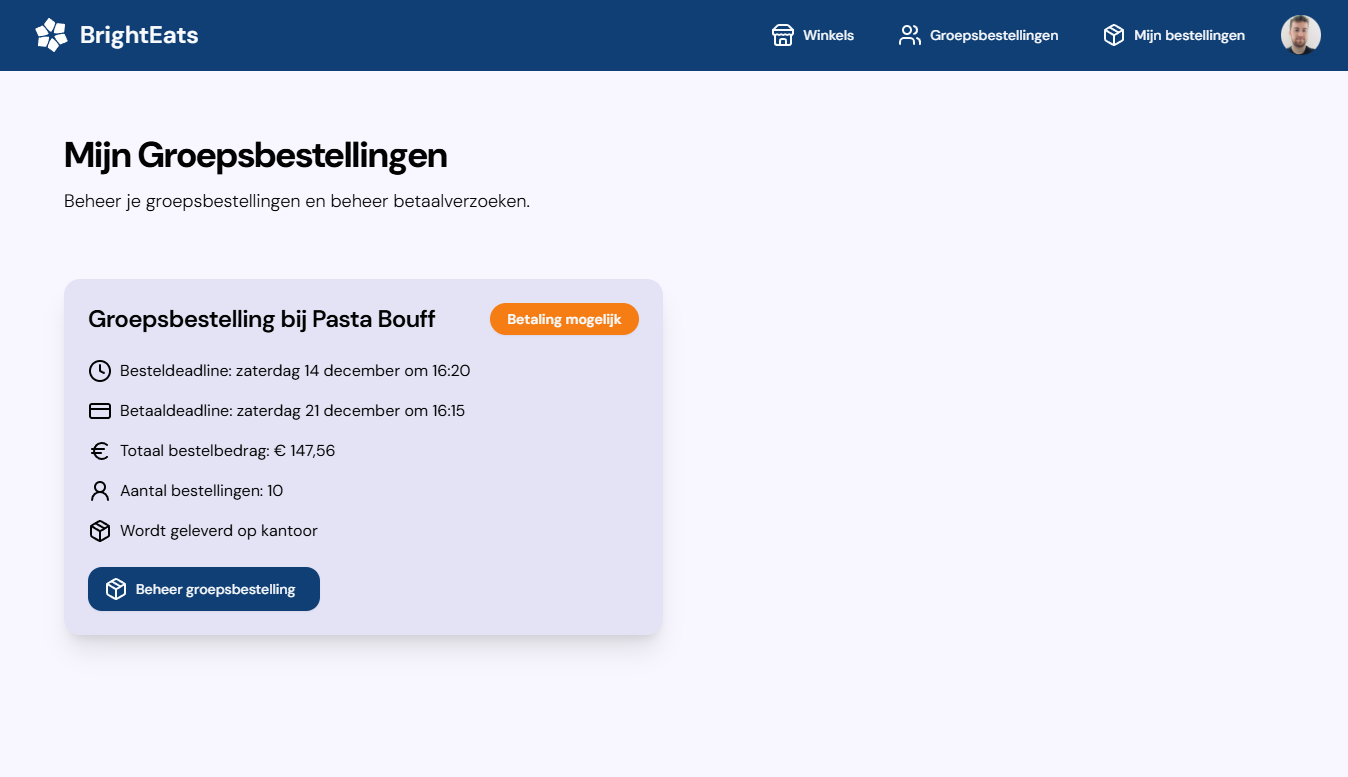
\includegraphics[width=0.8\textwidth]{my-group-orders-page.png}
\caption{Overzicht van group orders in de frontend}
\label{fig:group_orders_overview}
\end{figure}

\subsection{Conclusie}

De Vue.js frontend consumeert de \texttt{GroupOrder} resource via de \texttt{groupOrderService}, die de HTTP requests naar de API afhandelt. De TypeScript types in \texttt{types/group-order.ts} zorgen voor een duidelijke structuur van de data en maken type checking mogelijk. De componenten gebruiken de \texttt{groupOrderService} om data op te halen en te versturen, en verwerken de responses van de API. De conversiefuncties zorgen voor een correcte omzetting van het API formaat naar het frontend formaat.

Deze case study toont aan hoe de frontend en backend samenwerken om een consistente en gebruiksvriendelijke applicatie te realiseren. Door gebruik te maken van RESTful principes en een duidelijke structuur in zowel de frontend als de backend, wordt de ontwikkeling en het onderhoud van de applicatie simpel en efficiënt.

\section{OpenAPI}

Een belangrijk deel van onze RESTfulness guidelines is het gebruik van de OpenAPI-specificatie om de API te documenteren. Dit gaan we in deze sectie proberen te automatiseren. Er bestaan namelijk tools waarmee je de code van een Laravel-API automatisch kan omzetten naar een OpenAPI-specificatie. Wij gebruiken hiervoor de package \texttt{dedoc/scramble}.

\subsection{Problemen bij opzet}

Het opzetten van de documentatie was zeer simpel: we installeerden de package en stelden het configuratiebestand \texttt{scramble.php} in. Vervolgens starten we onze developmentomgeving en kregen we een mooie OpenAPI-specificatie te zien. Echter, bij het genereren van de specificatie van de BrightEats API, liepen we tegen enkele problemen aan.

\bigskip

Ten eerste was de API-documentatie niet heel uitgebreid. De documentatie bevatte enkel de endpoints en de parameters, maar miste beschrijvingen, voorbeelden en een algemene structuur. Deze moesten we toevoegen door middel van PHPDoc comments in de controllers, requests en resources.

\bigskip

Ten tweede was er het probleem dat Policies nog niet ondersteund worden. Daardoor moesten we zelf een creatieve manier vinden om op een mooie manier een kopje 'Authorization' toe te voegen aan de documentatie. Dit hebben we gedaan door in de PHPDoc comments van de controllers met markdown een kopje `Authorization' toe te voegen.

\bigskip

Het resultaat mag er zijn: een draaiende documentatiewebsite met alle endpoints, resources, validatieregels, authorisatieregels, voorbeelden en zelfs een interactieve terminal waarmee rechtstreeks met de API kan worden gecommuniceerd.

\begin{figure}[H]
\centering
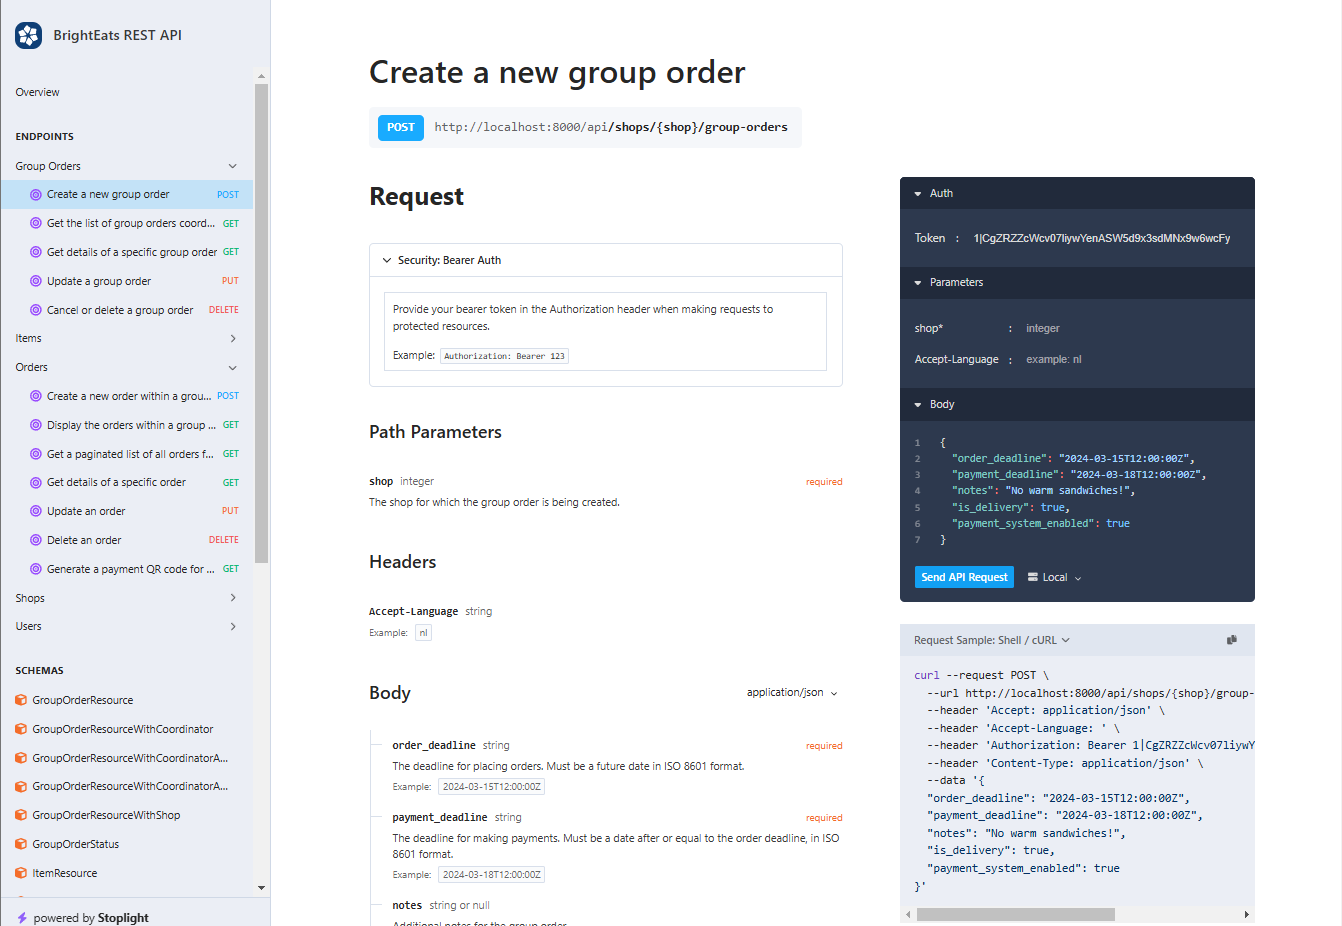
\includegraphics[width=0.8\textwidth]{scramble.png}
\caption{De OpenAPI documentatie van de BrightEats API}
\label{fig:openapi}
\end{figure}

\subsection{Conclusie}

Het automatisch genereren van de OpenAPI-specificatie van een Laravel-API is een krachtige tool om de API te documenteren en te delen met andere ontwikkelaars. De \texttt{dedoc/scramble} package biedt een eenvoudige manier om de API-specificatie te genereren en te hosten. Door de documentatie te verrijken met PHPDoc comments en markdown, kan de documentatie nog verder worden verbeterd. Het resultaat is een gestructureerde en gedetailleerde documentatie van de API, die kan worden gebruikt om de API te begrijpen en te integreren in andere applicaties.

\section{Conclusie}

In dit hoofdstuk hebben we de implementatie van een RESTful API en frontend voor de BrightEats applicatie besproken. We hebben de belangrijkste concepten en technieken behandeld die gebruikt zijn om een robuuste en schaalbare API te ontwikkelen. We hebben gekeken naar de structuur van de Laravel API, de Vue.js frontend, en hoe deze samenwerken om een volledige applicatie te vormen.

\bigskip

We hebben de implementatie van de \texttt{GroupOrder} resource in de backend en frontend geanalyseerd, en de verschillende onderdelen van de API en frontend besproken. We hebben gekeken naar de controllers, services, modellen, API resources, requests, policies, Axios configuratie, API services, data types, en componenten die betrokken zijn bij het beheren van groepsbestellingen.

\bigskip

Tot slot hebben we gekeken naar het genereren van de OpenAPI-specificatie voor de API met behulp van de \texttt{dedoc/scramble} package. We hebben de uitdagingen en oplossingen besproken bij het documenteren van de API en het toevoegen van beschrijvingen, voorbeelden en authorisatieregels aan de documentatie.

\bigskip

De implementatie van de BrightEats API en frontend illustreert hoe RESTful principes en best practices kunnen worden toegepast om een moderne en schaalbare applicatie te ontwikkelen. Door een duidelijke structuur en scheiding van verantwoordelijkheden te hanteren, wordt het onderhoud en de uitbreidbaarheid van de applicatie gegarandeerd. De documentatie van de API biedt een nuttige referentie voor het frontend team en andere ontwikkelaars die met de API willen integreren.


\chapter{Evaluatie}
\label{ch:evaluatie}

In dit hoofdstuk presenteren we de resultaten van de implementatie van de RESTful API principes en de OpenAPI-specificatie in de Bright\-Eats-applicatie. We evalu\-eren de impact van deze implementatie op de kwaliteit, consistentie en onderhoudbaarheid van de API, zowel vanuit het perspectief van de backend als de frontend. Om een grondige evaluatie uit te voeren, maken we gebruik van verschillende methoden, waaronder geautomatiseerde tests en een analyse van de ontwikkel- en onderhoudskosten. Aan de hand van deze resultaten zullen we de onderzoeksvragen beantwoorden en aanbevelingen formuleren voor toekomstige API-ontwikkelingen binnen BrightAnalytics.

\section{Consistentie}

Een consistente API is essentieel voor de bruikbaarheid en onderhoudbaarheid van de applicatie. In deze sectie evalu\-eren we de consistentie van de API endpoints, de datastructuren, de foutafhandeling en de documentatie.

\subsection{API endpoints}

Alle API endpoints in de Bright\-Eats-applicatie volgen de RESTful API principes. De endpoints zijn consistent benoemd en volgen de standaard conventies voor het gebruik van HTTP-methoden. De datastructuren van de request- en response bodies zijn uniform en voorspelbaar. De foutafhandeling is uniform en voorziet de gebruiker van voldoende informatie om de fout te identificeren en op te lossen. De documentatie is volledig en up-to-date en bevat alle informatie die nodig is om de API correct te gebruiken.

\subsection{HTTP Response Codes}

Een consistent gebruik van HTTP response codes is cruciaal voor een goede werking en begrijpelijkheid van de API. De Bright\-Eats API maakt gebruik van een reeks standaard HTTP response codes om de uitkomst van een request aan te geven. Over het algemeen worden de response codes consistent en correct toegepast.

\subsubsection{Succesvolle responses}

\begin{itemize}
  \item \textbf{200 OK:} Wordt gebruikt voor succesvolle GET, PUT, PATCH en DELETE requests. Bijvoorbeeld, wanneer een \texttt{GroupOrder} succesvol wordt opgehaald via \texttt{GET /group-orders/{groupOrder}}, wordt een 200 OK response met de \texttt{GroupOrder} data teruggestuurd.
  \item \textbf{201 Created:} Wordt gebruikt wanneer een resource succesvol is aangemaakt. Bijvoorbeeld, wanneer een nieuwe \texttt{GroupOrder} wordt aangemaakt via \texttt{POST /shops/{shop}/group-orders}, wordt een 201 Created response teruggestuurd, inclusief een \texttt{Location} header die verwijst naar de nieuwe \texttt{GroupOrder}.
  \item \textbf{204 No Content:} Wordt gebruikt wanneer een request succesvol is verwerkt, maar er geen content wordt teruggestuurd. Bijvoorbeeld, wanneer een \texttt{GroupOrder} succesvol wordt verwijderd via \texttt{DELETE /group-orders/{groupOrder}}, wordt een 204 No Content response teruggestuurd.
\end{itemize}

\subsubsection{Foutmeldingen}

\begin{itemize}
  \item \textbf{401 Unauthorized:} Wordt gebruikt wanneer de gebruiker niet geauthenticeerd is. Bijvoorbeeld, wanneer een niet-ingelogde gebruiker probeert om een lijst van \texttt{GroupOrders} op te halen, wordt een 401 Unauthorized response teruggestuurd.
  \item \textbf{403 Forbidden:} Wordt gebruikt wanneer de gebruiker niet geautoriseerd is om de actie uit te voeren. Bijvoorbeeld, wanneer een gebruiker probeert om een \texttt{GroupOrder} te verwijderen die niet door hem is gecoördineerd, wordt een 403 Forbidden response teruggestuurd.
  \item \textbf{404 Not Found:} Wordt gebruikt wanneer de opgevraagde resource niet bestaat. Bijvoorbeeld, wanneer een gebruiker probeert om een \texttt{GroupOrder} op te halen met een ID die niet bestaat, wordt een 404 Not Found response teruggestuurd.
  \item \textbf{409 Conflict:} Wordt gebruikt wanneer de request een conflict veroorzaakt met de huidige staat van de resource. Bijvoorbeeld, wanneer een admin probeert om een item toe te voegen aan de catalogus van een shop, maar het item bestaat al, wordt een 409 Conflict response teruggestuurd.
  \item \textbf{422 Unprocessable Entity:} Wordt gebruikt wanneer de request ongeldige data bevat. Bijvoorbeeld, wanneer bij het aanmaken van een \texttt{GroupOrder} de \texttt{order\_deadline} in het verleden ligt, wordt een 400 Bad Request response teruggestuurd met details over de validatiefout.
\end{itemize}

\subsubsection{Conclusie}

Over het algemeen worden de HTTP response codes in de Bright\-Eats API consistent en correct gebruikt. De codes geven duidelijk de uitkomst van een request aan en volgen de standaarden. Dit draagt bij aan de voorspelbaarheid en bruikbaarheid van de API. De responses zelf kunnen nog verbeterd worden. Zo kan een 400 response naast de algemene message ook specifieke errors per veld meegeven, en de 404 response een error code bevatten. Deze code is dan specifiek voor het falen van de authorisatie.

\section{Onderhoudbaarheid}

Een belangrijk aspect van een goed ontworpen API is de onderhoudbaarheid. Een onderhoudbare API is makkelijk aan te passen, uit te breiden en te debuggen. In deze sectie analyseren we de impact van de geïmplementeerde RESTful principes en de OpenAPI-specificatie op de onderhoudbaarheid van de Bright\-Eats API, met een specifieke focus op de tijd besteed aan debugging.

\subsection{Impact op Debugging Tijd}

Door de implementatie van RESTful principes en de OpenAPI-specificatie is de tijd die besteed wordt aan debugging significant verminderd. Dit is te danken aan verschillende factoren:

\begin{itemize}
\item \textbf{Gestructureerde code:} De duidelijke structuur van de code, met een scheiding van concerns door het gebruik van controllers, services, models, policies, requests en resources, maakt het eenvoudiger om de oorzaak van bugs te vinden. De code is beter leesbaar en makkelijker te volgen, waardoor ontwikkelaars snel kunnen navigeren naar de relevante secties.
\item \textbf{Consistente responses en foutafhandeling:} Het consistente gebruik van HTTP response codes en een uniforme structuur voor foutmeldingen maakt het makkelijker om problemen te identificeren en te diagnosticeren. Ontwikkelaars kunnen snel zien of een request succesvol was en, in geval van een fout, wat de oorzaak was.
\item \textbf{Automatisch gegenereerde documentatie:} De OpenAPI-specificatie genereert automatisch een interactieve API documentatie. Deze documentatie is altijd up-to-date en bevat gedetailleerde informatie over alle endpoints, inclusief request parameters, response bodies en mogelijke statuscodes. Dit maakt het eenvoudiger voor ontwikkelaars om te begrijpen hoe de API werkt en hoe ze deze moeten gebruiken, wat leidt tot minder fouten en snellere debugging.
\item \textbf{Voorspelbaarheid:} Dankzij de duidelijke structuur en de automatische docs kunnen we beter voorspellen wat de code zal doen en hoe de API zal reageren op verschillende requests. Dit helpt bij het voorkomen van bugs en maakt het makkelijker om bestaande bugs op te lossen.
\item \textbf{Robuustheid}: Door in de API zo veel mogelijk inkomende data toch te verwerken, ook als deze niet volledig aan de verwachtingen voldoet, is de API robuuster geworden. De API probeert bijvoorbeeld null waarden of ontbrekende velden zo goed mogelijk te interpreteren, in plaats van direct een foutmelding te geven. Dit heeft geresulteerd in het oplossen van enkele obscure bugs in de frontend, zonder dat de frontend code aangepast hoefde te worden. Hoewel dit extra implementatietijd kostte, heeft het de algehele onderhoudbaarheid verbeterd doordat de API toleranter is geworden voor kleine fouten in de requests.
\end{itemize}

\subsection{Impact op Toevoegen van nieuwe features}

De gestructureerde aanpak en het gebruik van duidelijke conventies maken het ook eenvoudiger om nieuwe features toe te voegen aan de API. Ontwikkelaars kunnen voortbouwen op de bestaande structuur en code, en de OpenAPI documentatie helpt hen om de impact van hun wijzigingen te begrijpen.

\subsection{Conclusie}

De implementatie van RESTful principes en de OpenAPI-specificatie heeft een positieve impact gehad op de onderhoudbaarheid van de Bright\-Eats API. De tijd besteed aan debugging is significant verminderd door de verbeterde structuur, consistentie, documentatie en voorspelbaarheid. Het toevoegen van nieuwe features is eenvoudiger geworden door de gestructureerde aanpak en het gebruik van conventies. De extra implementatietijd die nodig was om de API robuuster te maken, heeft zich terugbetaald in een vermindering van debugging tijd en een verhoogde stabiliteit van de applicatie.

\section{Kostenanalyse: OpenAPI-specificatie}

De implementatie van de OpenAPI-specificatie was een tijdsintensieve, maar waardevolle investering in de ontwikkeling van de Bright\-Eats API. In deze sectie analyseren we de kosten en baten van deze implementatie.

\subsection{Initiële Implementatiekosten}

Het toevoegen van de OpenAPI-specificatie bracht aanzienlijke initiële kosten met zich mee. De belangrijkste kostenpost was de tijd die nodig was om PHPDoc comments toe te voegen aan alle controllers, resources, requests en andere relevante klassen. Deze comments moesten gedetailleerde informatie bevatten over de datastructuren, parameters, en response types.

Deze initiële implementatie vereiste een aanzienlijke tijdsinvestering, maar was noodzakelijk om de basis te leggen voor een goed gedocumenteerde en onderhoudbare API.

\subsection{Voordelen op lange termijn}

Ondanks de hoge initiële kosten heeft de OpenAPI-specificatie op lange termijn aanzienlijke voordelen opgeleverd:

\begin{itemize}
  \item \textbf{Automatisch gegenereerde documentatie:} De OpenAPI-specificatie genereert automatisch een interactieve API documentatie. Deze documentatie is altijd up-to-date en bevat gedetailleerde informatie over alle endpoints, inclusief request parameters, response bodies en mogelijke statuscodes.
  \item \textbf{Verbeterde communicatie:} De OpenAPI documentatie dient als een centrale bron van waarheid voor zowel frontend- als backend-ontwikkelaars. Dit verbetert de communicatie tussen teams en vermindert misverstanden over de werking van de API.
  \item \textbf{Eenvoudigere debugging:} Zoals eerder vermeld in de sectie over onderhoudbaarheid, vergemakkelijkt de OpenAPI documentatie het debuggen van de API door een duidelijk overzicht te bieden van de verwachte input en output van elk endpoint.
  \item \textbf{Snellere onboarding van nieuwe developers:} Nieuwe developers kunnen sneller aan de slag met de API dankzij de uitgebreide en interactieve documentatie.
\end{itemize}

\subsection{Conclusie}

De implementatie van de OpenAPI-specificatie was een tijdsintensieve, maar waardevolle investering. De initiële kosten voor het toevoegen van PHPDoc comments en het configureren van de tools worden ruimschoots gecompenseerd door de voordelen op lange termijn. De automatisch gegenereerde, interactieve documentatie verbetert de communicatie, vereenvoudigt debugging, versnelt de onboarding van nieuwe developers en opent de deur naar codegeneratie en validatie. De OpenAPI-specificatie is daarmee een cruciale factor in de kwaliteit, consistentie en onderhoudbaarheid van de Bright\-Eats API.

\section{Testen}

Een cruciaal onderdeel van de ontwikkeling van de Bright\-Eats API was het implementeren van een uitgebreide testsuite. Alle API endpoints zijn grondig getest om de correcte werking van de API te garanderen en te valideren dat de implementatie voldoet aan de specificaties.

\subsection{Aanpak}

Voor het testen van de API is gebruik gemaakt van Pest, een modern testing framework voor PHP. Voor elk endpoint zijn meerdere test cases geschreven die verschillende scenario's afdekken, waaronder:

\begin{itemize}
  \item \textbf{Succesvolle requests:} Testen die verifiëren dat de API correct reageert op geldige requests met de verwachte statuscode en response body.
  \item \textbf{Foutieve requests:} Testen die verifiëren dat de API correct reageert op ongeldige requests, zoals requests met ontbrekende of foutieve parameters, met de juiste foutcodes en foutmeldingen.
  \item \textbf{Authenticatie en autorisatie:} Testen die verifiëren dat de API correct omgaat met authenticatie en autorisatie, en dat ongeautoriseerde gebruikers geen toegang hebben tot beveiligde endpoints.
  \item \textbf{Edge cases:} Testen die specifieke randgevallen afdekken, zoals het aanmaken van een \texttt{GroupOrder} met een \texttt{order\_deadline} die ver in de toekomst ligt of het bijwerken van een \texttt{GroupOrder} met conflicterende data.
\end{itemize}

Deze test cases zijn geïmplementeerd als Pest testmethoden, waarbij gebruik wordt gemaakt van Laravel's ingebouwde testing features, zoals het simuleren van HTTP requests en het inspecteren van de response.

\subsection{Voordelen}

Het schrijven van deze uitgebreide testsuite was een aanzienlijke investering, maar heeft zijn vruchten afgeworpen:

\begin{itemize}
\item \textbf{Kwaliteitsborging:} De tests hebben ervoor gezorgd dat eventuele bugs in een vroeg stadium werden ontdekt en opgelost. Dit heeft geresulteerd in een stabielere en betrouwbaardere API.
\item \textbf{Regressiepreventie:} Bij elke wijziging aan de API, hoe klein ook, worden alle tests automatisch uitgevoerd. Dit voorkomt regressie, waarbij bestaande functionaliteit onbedoeld kapot gaat door een wijziging.
\item \textbf{Vertrouwen bij refactoring:} De testsuite gaf het development team het vertrouwen om de API te refactoren en te optimaliseren, wetende dat de tests zouden aanslaan als er iets mis zou gaan. De uitgebreide tests maakten het mogelijk om met vertrouwen wijzigingen door te voeren. Dit bleek van onschatbare waarde tijdens het refactoren van de API. Zonder de zekerheid van de tests was het veel riskanter geweest om wijzigingen aan te brengen, met als mogelijk gevolg een minder optimale en minder onderhoudbare code.
\item \textbf{Levende documentatie:} De tests dienen ook als een vorm van levende documentatie, die laat zien hoe de API zich in verschillende situaties gedraagt.
\end{itemize}

\subsection{Conclusie}

Het grondig testen van alle API endpoints was een cruciale stap in de ontwikkeling van de Bright\-Eats API. De investering in het schrijven van de testsuite heeft zich ruimschoots terugverdiend in de vorm van een hogere kwaliteit, stabiliteit en onderhoudbaarheid van de API. De tests bieden een vangnet dat regressie voorkomt en het developmentteam in staat stelt om met vertrouwen te refactoren en de API verder te ontwikkelen.



%%=============================================================================
%% Conclusie
%%=============================================================================

\chapter{Conclusie}%
\label{ch:conclusie}

Dit hoofdstuk sluit deze bachelorproef af door de belangrijkste bevindingen samen te vatten en de centrale onderzoeksvraag te beantwoorden. Op basis van de resultaten en evaluatie uit het vorige hoofdstuk formuleren we concrete aanbevelingen voor de ontwikkeling van RESTful API's bij BrightAnalytics, met focus op het verbeteren van kwaliteit, consistentie en onderhoudbaarheid.

\bigskip

De implementatie van RESTful API principes en de OpenAPI specificatie in de Bright\-Eats API heeft geleid tot significante verbeteringen op verschillende vlakken:

\begin{itemize}
  \item \textbf{Kwaliteit:} De kwaliteit van de API is aanzienlijk verbeterd door de implementatie van geautomatiseerde tests en een focus op robuustheid. De API is stabieler, betrouwbaarder en beter bestand tegen fouten.
  \item \textbf{Consistentie:} De API is consistent in design en implementatie dankzij de strikte naleving van RESTful principes en het gebruik van onze opgestelde guidelines. De endpoints zijn uniform ontworpen, HTTP response codes worden correct gebruikt en datastructuren zijn voorspelbaar. Er is nog ruimte voor verbetering in de responses zelf.
  \item \textbf{Onderhoudbaarheid:} De onderhoudbaarheid van de API is sterk verbeterd door de gestructureerde code, de uitgebreide documentatie en de test suite. De tijd besteed aan debugging is verminderd en het toevoegen van nieuwe features is eenvoudiger geworden.
\end{itemize}

De implementatie van de OpenAPI specificatie was de grootste kostenpost, met name de tijd die nodig was om PHPDoc comments toe te voegen aan de code. Deze initiële investering heeft zich echter terugbetaald in de vorm van automatisch gegenereerde documentatie, verbeterde communicatie, eenvoudigere debugging en snellere onboarding van nieuwe developers.

\bigskip

De evaluatie van de Bright\-Eats API toont aan dat de implementatie van RESTful API principes en de OpenAPI specificatie een positieve impact heeft op de kwaliteit, consistentie en onderhoudbaarheid van de API. De API is stabieler, betrouwbaarder en beter bestand tegen fouten. De endpoints zijn uniform ontworpen, HTTP response codes worden correct gebruikt en datastructuren zijn voorspelbaar. De onderhoudbaarheid van de API is sterk verbeterd door de gestructureerde code, de uitgebreide documentatie en de test suite.

\section{Antwoord op de onderzoeksvraag}

De centrale onderzoeksvraag van deze bachelorproef luidt als volgt:

\begin{displayquote}
  \textit{Welke concrete voordelen biedt de implementatie van RESTful API design, en in het bijzonder HATEOAS en OpenAPI, voor de kwaliteit, consistentie en onderhoudbaarheid van een Laravel-API en een bijbehorende frontend applicatie?}
\end{displayquote}

Op basis van de bevindingen uit dit onderzoek kunnen we deze vraag als volgt beantwoorden:

\subsection{RESTful API design}

De implementatie van RESTful API design principes heeft een positieve impact gehad op de kwaliteit, consistentie en onderhoudbaarheid van de Bright\-Eats Laravel-API. De gestructureerde aanpak, met een duidelijke scheiding van concerns (controllers, services, models), een consistent gebruik van HTTP methoden en status codes, en de toepassing en opstelling van een set duidelijke guidelines, heeft geresulteerd in een robuuste, voorspelbare en makkelijk te begrijpen API. Dit heeft op zijn beurt geleid tot een verhoogde kwaliteit van de code, een snellere ontwikkeling en een verbeterde onderhoudbaarheid.

\subsection{HATEOAS}

De beslissing om HATEOAS \textit{niet} te implementeren bleek de juiste te zijn. De meerwaarde van HATEOAS in het geval van de Bright\-Eats API, die enkel intern bij BrightAnalytics gebruikt wordt, woog niet op tegen de complexiteit en overhead die gepaard gaan met de implementatie ervan. De uitgebreide documentatie gegenereerd door OpenAPI, in combinatie met de duidelijke communicatie binnen het development team, biedt voldoende mogelijkheden voor ontwikkelaars om de API te begrijpen en te gebruiken.

\subsection{OpenAPI}

OpenAPI heeft een cruciale rol gespeeld in het verbeteren van de documentatie en standaardisatie van de API. De automatisch gegenereerde, interactieve documentatie dient als een centrale bron van waarheid voor alle ontwikkelaars en vereenvoudigt de samenwerking tussen frontend en backend teams. Bovendien opent OpenAPI de mogelijkheid voor toekomstige automatisering, zoals het genereren van client SDK's en het valideren van requests en responses.

\section{Aanbevelingen}

De aanbevelingen voor API design bij BrightAnalytics zijn opgesteld in hoofdstuk 4 van deze bachelorproef. Hier gaan we concreet bepalen wat een RESTful API is en zorgen we voor minder ambigu\"iteit in API responses, requests, query parameters, foutafhandeling, caching en versiebeheer. Dit document dient een startpunt te worden voor een goede set guidelines die in het algemeen kunnen worden gebruikt voor het bouwen van performante, robuuste en onderhoudbare API's.

\bigskip

Niet alle guidelines die werden opgesteld in dit onderzoek zijn even relevant voor elk project. Voor Bright\-Eats bijvoorbeeld hebben we de meer geavanceerde guidelines over query parameters, filters en sortering niet moeten implementeren. Voor andere projecten zullen andere delen van de guidelines minder of meer relevant zijn. Het is belangrijk om de guidelines te zien als een set van best practices die kunnen worden aangepast aan de specifieke noden van elk project.

\bigskip

Daarnaast raden we aan om de implementatie van OpenAPI verder te onderzoeken en te integreren in de bestaande ontwikkelprocessen. De voordelen van automatisch gegenereerde documentatie, standaardisatie en automatisering wegen op tegen de initi\"ele investering die nodig is om de specificatie op te stellen. Het is belangrijk om de documentatie up-to-date te houden en te integreren in de dagelijkse workflow van de ontwikkelaars. Op die manier wordt de documentatie een levend document dat een centrale bron van waarheid vormt voor alle betrokken partijen.

\section{Reflectie en toekomstig onderzoek}

Het onderzoeksproces verliep over het algemeen vlot. De iteratieve aanpak, waarbij de API stapsgewijs werd ontwikkeld en getest, bleek effectief. De keuze om vroeg in het proces te focussen op OpenAPI heeft de documentatie en consistentie van de API sterk verbeterd.

\bigskip

Een punt van verbetering is de diepgang van de evaluatie van de onderhoudskosten. Hoewel de tijd besteed aan debugging is afgenomen naarmate de API meer RESTful werd, is het lastig om dit exact te kwantificeren. Een meer gedetailleerde tracking van de ontwikkeltijd had hier meer inzicht in kunnen geven.

\bigskip

Een beperking van dit onderzoek is de focus op een specifieke use case, namelijk de Bright\-Eats API. De bevindingen zijn mogelijk niet generaliseerbaar naar andere API's of andere contexten.

\subsection{Suggesties voor toekomstig onderzoek}

\begin{itemize}
  \item \textbf{Langetermijnevaluatie:} Een evaluatie van de impact van RESTful API design en OpenAPI op de onderhoudskosten op langere termijn zou waardevolle inzichten kunnen opleveren.
  \item \textbf{Vergelijking met andere API-stijlen:} Een vergelijking van de RESTful aanpak met andere API stijlen, zoals GraphQL, zou interessant zijn om de voor- en nadelen van elke stijl beter te begrijpen.
  \item \textbf{Automatische validatie met OpenAPI:} Verder onderzoek naar het gebruik van OpenAPI voor het automatisch valideren van requests en responses zou de robuustheid van API's kunnen verhogen.
  \item \textbf{API-beveiliging:} Een diepere analyse van de implementatie van API security maatregelen zou een belangrijke toevoeging zijn aan toekomstig onderzoek.
  \item \textbf{Performance testen:} Onderzoek naar de performance implicaties van verschillende API design keuzes zou waardevol zijn voor het optimaliseren van de API performance.
\end{itemize}

\section{Afsluiting}

Goed API-ontwerp is essentieel voor het succes van moderne software applicaties. Een goed ontworpen API is niet alleen robuust, consistent en onderhoudbaar, maar ook makkelijk te gebruiken en te integreren met andere systemen. Deze bachelorproef heeft aangetoond dat de implementatie van RESTful API principes en de OpenAPI specificatie een significante bijdrage levert aan het bereiken van deze doelen. De aanbevelingen in deze bachelorproef bieden BrightAnalytics concrete handvatten voor het ontwikkelen van hoogwaardige API's, wat de efficiëntie van het development team verhoogt en de kwaliteit van de software verbetert.


%---------- Bijlagen -----------------------------------------------------------

\appendix

\chapter{Onderzoeksvoorstel}

Het onderwerp van deze bachelorproef is gebaseerd op een onderzoeksvoorstel dat vooraf werd beoordeeld door de promotor. Dat voorstel is opgenomen in deze bijlage.

%% TODO: 
%\section*{Samenvatting}

% Kopieer en plak hier de samenvatting (abstract) van je onderzoeksvoorstel.

% Verwijzing naar het bestand met de inhoud van het onderzoeksvoorstel
%---------- Inleiding ---------------------------------------------------------

\section{Inleiding}%
\label{sec:inleiding}
De explosieve groei van data en de toenemende vraag naar naadloze integraties tussen applicaties hebben de rol van Application Programming Interfaces (API's) centraal geplaatst in de hedendaagse softwareontwikkeling. Een goed ontworpen en gedocumenteerde API is niet langer een luxe, maar essentieel voor succes in het digitale landschap. Dit is met name relevant voor BrightAnalytics, een bedrijf dat een geavanceerd data-visualisatieplatform aanbiedt voor financiële rapportering en business intelligence. De kwaliteit, consistentie en efficiëntie van de API's die BrightAnalytics ontwikkelt, zijn van cruciaal belang voor de functionaliteit van hun producten, de integratie met andere systemen en het snel kunnen ontwikkelen van nieuwe features.

\bigskip

Tijdens mijn stage bij BrightAnalytics ontwikkel ik "BrightEats", een applicatie waarmee werknemers hun lunch kunnen bestellen. Deze applicatie is afhankelijk van een backend API, geschreven in Laravel, net zoals alle andere applicaties bij BrightAnalytics. De ontwikkeling van deze API biedt een uitgelezen kans om de principes van RESTful API design te implementeren en om te evalueren welke voor- en nadelen de meer geavanceerde principes hiervan (met name OpenAPI en Hypermedia As The Engine Of Application State (HATEOAS) ) met zich meebrengen.

\bigskip

Het principe van RESTful API design werd in 2000 geïntroduceerd door Roy Fielding in zijn proefschrift \autocite{Fielding2000}. REST (Representational State Transfer) is ondertussen wijdverspreid en wordt goed ondersteund wanneer we een API willen bouwen met Laravel. Echter zijn de meer geavanceerde onderdelen van REST, met name HATEOAS (Hypermedia As The Engine Of Application State) en OpenAPI, minder bekend en worden ze minder vaak toegepast in de praktijk. Deze principes kunnen echter een grote impact hebben op de kwaliteit, consistentie en onderhoudbaarheid van een API.

\bigskip

Met deze bachelorproef proberen we een antwoord te formuleren op de volgende onderzoeksvraag:

\begin{center}
\textbf{Welke concrete voordelen biedt de implementatie van RESTful API design, en in het bijzonder HATEOAS en OpenAPI, voor de kwaliteit, consistentie en onderhoudbaarheid van een Laravel-API en een bijbehorende frontend applicatie?}
\end{center}

\bigskip

We moeten hiervoor volgende deelvragen beantwoorden:

\begin{itemize}
  \item Wat zijn de principes van RESTful API design en hoe dragen deze bij aan betere API's?
  \item Wat is HATEOAS en hoe kan dit principe worden toegepast in een Laravel-API?
  \item Wat is OpenAPI en hoe kan dit worden toegepast in de documentatie van een Laravel-API?
  \item Welke concrete voordelen biedt de implementatie van deze principes voor de kwaliteit, consistentie en onderhoudbaarheid van de BrightEats API?
  \item Hoeveel aanpassingen zijn er nodig in de frontend applicatie om te kunnen werken met een HATEOAS API? Draagt dit bij aan de onderhoudbaarheid van deze applicatie?
\end{itemize}

Deze vragen zullen beantwoord worden aan de hand van de volgende onderzoeksdoelstellingen:

\bigskip

\begin{enumerate}
\item \textbf{Inzicht verwerven in RESTful API design:} Een diepgaande analyse van de principes van RESTful API design, HATEOAS en OpenAPI specificatie, om deze zo goed mogelijk te kunnen toepassen en evalueren. We gaan ook na hoe we dit kunnen implementeren in een Laravel-API.
\item \textbf{Ontwikkeling API en bijbehorende front-end:} Het ontwikkelen en refactoren van de BrightEats API naar deze standaarden om zo de voor- en nadelen te kunnen evalueren. Hierbij gaan we ook de impact op de frontend applicatie evalueren.
\item \textbf{Formuleren van aanbevelingen:} Op basis van de bevindingen tijdens de implementatie nagaan welke principes van RESTful API design, HATEOAS en OpenAPI nuttig zijn voor BrightAnalytics en hoe deze best kunnen worden toegepast in de praktijk.
\end{enumerate}

\bigskip

Deze bachelorproef is relevant voor BrightAnalytics, omdat we kunnen nagaan of het implementeren van HATEOAS en OpenAPI in API's effectief een meerwaarde biedt. Ook is het interessant om na te gaan welke kosten en moeite er gepaard gaan met het implementeren van deze principes en of deze opwegen tegen de voordelen. Hoe compatibel zijn deze principes met de tech stack (Laravel, Vue.js) van BrightAnalytics en welke best practices kunnen worden geformuleerd voor de implementatie hiervan?

\section{Literatuurstudie}%
\label{sec:literatuurstudie}

REST (Representational State Transfer) is een veelgebruikte architectuur om API's te ontwerpen en bouwen \autocite{Eddouibi2017}. Die populariteit heeft REST te danken aan zijn eenvoud, schaalbaarheid en compatibiliteit met de standaarden van het internet. Dankzij REST kunnen ontwikkelaars op een flexibele en efficiënte manier API's bouwen die vlot kunnen omgaan met de almaar toenemende hoeveelheid data die bedrijven vandaag genereren. In de volgende secties zullen we dieper ingaan op de principes en voordelen van RESTful API's.

\subsection{De principes van RESTful API's}

RESTful API's zijn gebaseerd op een aantal belangrijke principes die bijdragen aan hun eenvoud, schaalbaarheid en gebruiksvriendelijkheid. Eén van die principes is de client-server architectuur \autocite{Fielding2000}. Een RESTful API maakt een duidelijke scheiding tussen de client, die een aanvraag doet (bijvoorbeeld een rapport opvragen), en de server, die de aanvraag verwerkt en een antwoord terugstuurt. Deze scheiding zorgt ervoor dat de client en server onafhankelijk van elkaar kunnen evolueren, wat de flexibiliteit en onderhoudbaarheid ten goede komt.

\bigskip

Een ander belangrijk principe is statelessness, wat betekent dat elke request van de client naar de server alle informatie bevat die nodig is om de request te verwerken \autocite{Fielding2000}. De server hoeft dus geen informatie over de client bij te houden tussen verschillende requests. Dit maakt RESTful API's schaalbaarder, omdat servers requests parallel kunnen verwerken zonder afhankelijk te zijn van eerdere interacties. Bovendien wordt de betrouwbaarheid verhoogd, omdat een servercrash geen dataverlies veroorzaakt aan de clientzijde.

\bigskip

Cacheability is een derde belangrijk principe van REST  \autocite{Fielding2000}. Responses van de server kunnen gemarkeerd worden als cacheable, wat betekent dat de client (of een tussenliggende server) de response mag opslaan en hergebruiken voor latere, identieke requests. Caching vermindert de belasting van de server en verkort de laadtijden voor de gebruiker, wat de performantie van de applicatie ten goede komt.

\bigskip

Een uniform interface is een ander cruciaal aspect van RESTful API's. Dit betekent dat alle resources (bijvoorbeeld financiële rapporten, klanten, transacties) benaderd worden via eenzelfde set van operaties, gedefinieerd door de HTTP-methodes (GET, POST, PUT, PATCH, DELETE) \autocite{Fielding2000}. Deze uniformiteit maakt de API voorspelbaar en gemakkelijk te gebruiken, omdat ontwikkelaars niet hoeven te leren hoe ze met elk type resource op een andere manier moeten omgaan.

\bigskip

Tot slot is het principe van een gelaagde systeemarchitectuur ook van toepassing op RESTful API's \autocite{Fielding2000}. Dit betekent dat de API kan worden opgebouwd uit verschillende lagen die elk een specifieke verantwoordelijkheid hebben. Zo kan er bijvoorbeeld een laag zijn die instaat voor authenticatie en autorisatie, een laag die data ophaalt uit de database en een laag die de data omzet naar het gewenste formaat. Deze gelaagdheid bevordert de modulariteit en herbruikbaarheid van code, wat de onderhoudbaarheid en schaalbaarheid van de API ten goede komt.

\bigskip

Door deze principes te volgen, dragen RESTful API's bij aan het creëren van software die flexibeler, schaalbaarder, betrouwbaarder en gebruiksvriendelijker is. 

\subsection{HATEOAS: flexibiliteit en dynamische navigatie}

Eén van de krachtigste eigenschappen van RESTful API's is hun flexibiliteit. Een goed ontworpen RESTful API kan gemakkelijk evolueren en uitbreiden zonder dat bestaande toepassingen die er gebruik van maken, moeten worden aangepast. HATEOAS (Hypermedia As The Engine Of Application State) is een belangrijk concept binnen REST dat deze flexibiliteit nog verder vergroot.

\bigskip

Bij de HATEOAS-aanpak bevatten de antwoorden van de API niet alleen de gevraagde data, maar ook links naar gerelateerde resources en acties die de gebruiker kan uitvoeren \autocite{Aydemir_2022}. Stel je bijvoorbeeld voor dat een gebruiker via een API een rapport opvraagt over maandelijkse verkoopcijfers. In een traditionele API zou het antwoord enkel de data van het rapport bevatten. Maar met HATEOAS zou het antwoord ook links kunnen bevatten om:

\begin{itemize}
  \item De data van het rapport te downloaden in een ander formaat (bijvoorbeeld CSV, Excel);
  \item Een nieuw rapport te genereren voor een andere periode;
  \item De onderliggende data van het rapport te bekijken;
  \item De toegang tot het rapport aan te passen.
\end{itemize}

\bigskip

Door deze links te volgen, kan een client op een dynamische manier door de API navigeren en verschillende acties uitvoeren, zonder dat de ontwikkelaar van de client op voorhand alle mogelijke URI's van de API moet kennen. Dit maakt de API flexibeler en minder foutgevoelig voor veranderingen. Als de structuur van de API in de toekomst verandert, hoeven enkel de links in de responses te worden aangepast, zonder dat de client-applicaties zelf moeten worden bijgewerkt.

\bigskip

HATEOAS wordt beschouwd als een essentieel onderdeel van een "volwassen" RESTful API en draagt bij aan de loose coupling tussen client en server, wat de onderhoudbaarheid en schaalbaarheid van de API ten goede komt.

\subsection{OpenAPI: Documentatie en standaardisatie}

Een goed gedocumenteerde API is essentieel voor ontwikkelaars die de API willen gebruiken. Zonder duidelijke documentatie is het moeilijk om te weten hoe je de API moet aanspreken, welke data je kunt opvragen en welke parameters je moet meegeven. OpenAPI (vroeger bekend als Swagger) biedt een oplossing voor dit probleem door een gestandaardiseerde manier te bieden om RESTful API's te documenteren.

\bigskip

OpenAPI is een specificatie die beschrijft hoe je een RESTful API kunt documenteren in een machine-leesbaar formaat, meestal YAML of JSON \autocite{Swagger2021}. Een OpenAPI-document bevat een gedetailleerde beschrijving van alle endpoints, parameters, requests, responses en datatypen die de API gebruikt.

\bigskip

Het gebruik van OpenAPI biedt tal van voordelen voor zowel API-ontwikkelaars als -gebruikers. Zo kan er op basis van een OpenAPI-document automatisch documentatie worden gegenereerd in een gebruiksvriendelijk formaat, bijvoorbeeld met behulp van tools zoals Swagger UI of Redoc \autocite{Swagger2021}. Dit bespaart ontwikkelaars heel wat tijd en moeite, en zorgt ervoor dat de documentatie altijd up-to-date is met de laatste versie van de API.

\subsection{Best practices voor API design}

Een API moet niet alleen functioneel zijn, maar ook gebruiksvriendelijk, flexibel en performant, zodat ontwikkelaars er vlot mee kunnen werken. Daarom is het belangrijk om te steunen op beproefde best practices bij het ontwerp en de implementatie van een API.

\bigskip

Eén van de belangrijkste aspecten is het gebruik van duidelijke en consistente naamgevingsconventies voor URI's (Uniform Resource Identifiers), die de verschillende resources van de API identificeren. Het is aangeraden om zelfstandige naamwoorden in het meervoud te gebruiken, bijvoorbeeld `/api/v1/orders` om alle bestellingen op te halen, of `/api/v1/orders/123` om een specifieke bestelling met ID 123 op te halen \autocite{Lange2024}. Door consistente naamgevingsconventies te hanteren, wordt de API voorspelbaarder en gemakkelijker te gebruiken.

\bigskip

Het correct gebruiken van HTTP-methoden (GET, POST, PUT, DELETE) is essentieel voor een RESTful API \autocite{Lange2024}. Elke methode heeft een specifieke betekenis en wordt gebruikt voor een ander type actie. Zo wordt GET gebruikt om data op te vragen, POST om nieuwe resources aan te maken, PUT om bestaande resources te overschrijven en DELETE om resources te verwijderen. Door de juiste methode te gebruiken voor elke actie, wordt de API semantisch correct en consistent met de REST-principes.

\bigskip

De performance van de API is ook van cruciaal belang. Gebruikers verwachten dat data snel en soepel wordt ingeladen, en lange laadtijden kunnen leiden tot frustratie en een slechte gebruikerservaring. Daarom is het belangrijk om bij het ontwerp van de API rekening te houden met factoren die de performantie kunnen beïnvloeden, zoals de grootte van de datasets, de complexiteit van de queries en de efficiëntie van de data-uitwisseling. Technieken zoals caching, paginering en compressie kunnen helpen om de performantie te verbeteren en de laadtijden te verkorten.

\bigskip

Tot slot is een duidelijke en uitgebreide documentatie onmisbaar. De documentatie moet niet alleen de technische details van de API beschrijven, maar ook voorbeelden en use cases bevatten die ontwikkelaars helpen om de API snel en efficiënt te integreren in hun eigen applicaties. Met behulp van OpenAPI is dit proces geautomatiseerd en gestandaardiseerd, wat de consistentie en duidelijkheid van de documentatie ten goede komt.

\subsection{Conclusie}

In een wereld gedreven door data zijn API's onmisbaar geworden om de kloof tussen verschillende softwareoplossingen te overbruggen en naadloze gegevensuitwisseling mogelijk te maken. REST, gebaseerd op een reeks krachtige principes zoals client-server architectuur, statelessness en een uniforme interface, heeft zich bewezen als een robuuste en flexibele oplossing voor het ontwerpen van API's.

\bigskip

Het hanteren van best practices, zoals duidelijke URI-structuren, correct gebruik van HTTP-methoden en een doordachte beveiliging, is essentieel voor het creëren van API's die niet alleen functioneel zijn, maar ook gebruiksvriendelijk en veilig.

\bigskip

HATEOAS voegt een extra laag van flexibiliteit toe aan RESTful API's door clients in staat te stellen dynamisch te navigeren en te interageren met resources via hyperlinks. OpenAPI biedt een gestandaardiseerde manier om API's te documenteren, wat de ontwikkeling en het gebruik ervan vergemakkelijkt.

%---------- Methodologie ------------------------------------------------------
\section{Methodologie}
\label{sec:methodologie}

Deze bachelorproef onderzoekt en verbetert de API-kwaliteit bij BrightAnalytics door de iteratieve ontwikkeling van de BrightEats API. Onderzoek en ontwikkeling gaan hand in hand. De inzichten uit het onderzoek worden direct toegepast op de API, en de ervaringen tijdens de ontwikkeling sturen het onderzoek bij.

\bigskip
Ik ga ervan uit dat ik elke week minstens \'e\'en dag kan werken aan de bachelorproef. De deadlines zijn echter flexibel, aangezien de API-ontwikkeling continu doorloopt en de planning kan be\"invloeden.

\subsection{Fase 1: Onderzoek en eerste opzet API}

\textbf{Deadline: 3 november 2024}

\bigskip
Deze fase is gericht op het verzamelen van kennis over kwalitatieve API-ontwikkeling en het defini\"eren van een eerste set best practices voor BrightEats. Ik bestudeer de principes van REST, HATEOAS en OpenAPI en hun belang voor API-kwaliteit en formuleer concrete aanbevelingen voor de BrightEats API.

\bigskip

\textbf{We zoeken een antwoord op de volgende vragen:}
\begin{itemize}
  \item Wat zijn de principes van REST?
  \item Hoe dragen deze bij aan betere API's?
  \item Welke best practices zijn er voor URI-structuur, HTTP-methoden, response codes en versiebeheer?
  \item Hoe houden we onze Laravel-API RESTful?
  \item Wat zijn de principes en voordelen van HATEOAS?
  \item Hoe kunnen we HATEOAS implementeren in een Laravel-API?
  \item Hoe maken we optimaal gebruik van HATEOAS in de frontend van BrightEats?
  \item Wat is OpenAPI en hoe kan dit worden toegepast in de documentatie van een Laravel-API?
\end{itemize}

\textbf{Deliverables:}

\begin{itemize}
  \item Literatuurstudie over REST, HATEOAS en OpenAPI.
  \item Best practices voor de implementatie hiervan in de BrightEats API en frontend.
\end{itemize}

\subsection{Fase 2: Iteratieve ontwikkeling en verfijning BrightEats API}

\textbf{Deadline: 8 december 2024}

\bigskip
Gedurende deze fase ontwikkel ik de BrightEats API iteratief en verfijn ik de best practices. We kijken welke principes nuttig zijn in de praktijk en welke aanpassingen nodig zijn om deze te implementeren in de BrightEats API.

\subsubsection{Ontwikkeling van de API (doorlopend)}

\bigskip
Elke week doorloop ik de volgende stappen:

\begin{enumerate}
  \item \textbf{Plannen:} Ik bepaal welke functionaliteiten ik aan de API zal toevoegen (of welke code ik ga refactoren om zo aan de nieuwe best practices te voldoen)
  \item \textbf{Ontwerpen:} Ik ontwerp de nieuwe functionaliteiten met de best practices in gedachten.
  \item \textbf{Implementeren:} Ik programeer de nieuwe functionaliteiten in de API.
  \item \textbf{Testen:} Ik test de nieuwe functionaliteiten grondig.
  \item \textbf{Evalueren:} Ik beoordeel de kwaliteit, structuur en gebruikte best practices.
  \item \textbf{Best practices bijstellen:} Ik pas de richtlijnen aan op basis van de evaluatie en feedback.
\end{enumerate}

\textbf{Deliverables:}

\begin{itemize}
  \item Wekelijkse updates van de BrightEats API.
  \item Documentatie van de API met OpenAPI specificaties.
  \item Logboek met gemaakte keuzes en evaluaties.
\end{itemize}

\subsection{Fase 3: Synthese, aanbevelingen en afronding}

\textbf{Deadline: 15 december 2025}

\bigskip
In de laatste fase vat ik mijn bevindingen samen en formuleer ik een antwoord op de onderzoeksvraag. Wat was de exacte kost van het implementeren van HATEOAS en OpenAPI in de BrightEats API? Welke voordelen en nadelen bracht dit met zich mee? Welke best practices kunnen we formuleren voor de ontwikkeling van API's bij BrightAnalytics?

\subsubsection{Synthese \& Aanbevelingen}

\textbf{Deadline: 15 januari 2025}

\bigskip
Ik schrijf de conclusie en aanbevelingen voor BrightAnalytics. Hierbij beantwoord ik de deelvragen en onderzoeksvraag en formuleer ik concrete best practices voor de ontwikkeling van RESTful API's bij BrightAnalytics.

\subsubsection{Afronding bachelorproef}

\textbf{Deadline: 10 januari 2025}

\bigskip
Ik werk de bachelorproef af, rekening houdend met de feedback van de promotor en de lead developer bij BrightAnalytics.

\textbf{Deliverables:}

\begin{itemize}
  \item Concrete aanbevelingen voor beter API-ontwerp.
  \item Finale versie van de bachelorproef.
\end{itemize}

\subsection{Gantt chart}

In figuur 1 vind je een overzicht van de planning van de bachelorproef. Hierin zie je de verschillende fases en deadlines.

%---------- Verwachte resultaten ----------------------------------------------
\section{Verwachte resultaten en conclusie}%
\label{sec:verwachte_resultaten}

Gebaseerd op de voordelen van REST, HATEOAS en OpenAPI die in de literatuurstudie beschreven zijn, verwacht ik dat de implementatie van deze principes in de BrightEats API zal leiden tot een hogere kwaliteit, consistentie en onderhoudbaarheid, wat zich zal uiten in:

\subsection{Kwaliteit}

\begin{itemize}
    \item \textbf{Verbeterde structuur en leesbaarheid:} De API zal een duidelijk gedefinieerde structuur hebben die consistent is met de RESTful principes, waardoor deze beter leesbaar wordt voor ontwikkelaars. Dit evalueer ik door de API te laten reviewen door andere developers. Ik verwacht positieve feedback te krijgen over de overzichtelijkheid en structuur.
    \item \textbf{Verbeterde DX (Developer Experience):} De API zal gemakkelijker te gebruiken zijn voor ontwikkelaars, dankzij de consistente naamgevingsconventies, uniforme datamodellen en duidelijke documentatie. Ik verwacht dat ontwikkelaars die met de API werken, minder tijd zullen besteden aan het uitzoeken van de werking en meer tijd zullen kunnen besteden aan het ontwikkelen van nieuwe features.
\end{itemize}

\subsection{Consistentie}

\begin{itemize}
    \item \textbf{Eenduidige naamgevingsconventies:} De API zal gebruik maken van consistente naamgevingsconventies voor URI's, resources en parameters, waardoor deze voorspelbaarder en gemakkelijker te gebruiken zal zijn. Ik verwacht dat ontwikkelaars die voor het eerst met de API werken, snel vertrouwd zullen zijn met de structuur en naamgeving.
    \item \textbf{Uniformiteit in gebruikte datamodellen:} De data die door de API wordt uitgewisseld zal consistent zijn in structuur en formaat, wat de integratie met andere systemen zal vergemakkelijken.
\end{itemize}

\subsection{Onderhoudbaarheid}

\begin{itemize}
    \item \textbf{Verbeterde documentatie:} Dankzij OpenAPI specificaties zal de API automatisch gedocumenteerd worden, waardoor de documentatie altijd up-to-date zal zijn en ontwikkelaars snel en gemakkelijk informatie over de API kunnen vinden.
    \item \textbf{Eenvoudiger onderhoud en uitbreiding:} De modulaire opbouw van de API en de duidelijke scheiding tussen client en server zullen het onderhoud en de uitbreiding van de API vergemakkelijken. Ik verwacht dat nieuwe functionaliteiten sneller en efficiënter aan de API kunnen worden toegevoegd.
\end{itemize}

\subsection{Conclusie}

Deze bachelorproef zal nagaan of de voordelen van RESTful API design, HATEOAS en OpenAPI opwegen tegen de nadelen, en of deze aanpak in de praktijk haalbaar en nuttig is in de tech stack van BrightAnalytics. De resultaten van deze bachelorproef zijn relevant, aangezien we zo weten of met name HATEOAS wel degelijk een meerwaarde biedt voor de API's van BrightAnalytics. De best practices die geformuleerd worden, zullen nuttig zijn voor toekomstige API-ontwikkeling binnen BrightAnalytics.

De BrightEats API zal dienen als een showcase voor deze best practices en als blauwdruk voor toekomstige API-ontwikkeling. Indien het implementeren van deze principes echter te complex of tijdrovend blijkt te zijn, kan dit een signaal zijn dat de voordelen niet opwegen tegen de nadelen en dat er andere oplossingen moeten worden gezocht.

\clearpage

\begin{figure}[H]
  \centering
  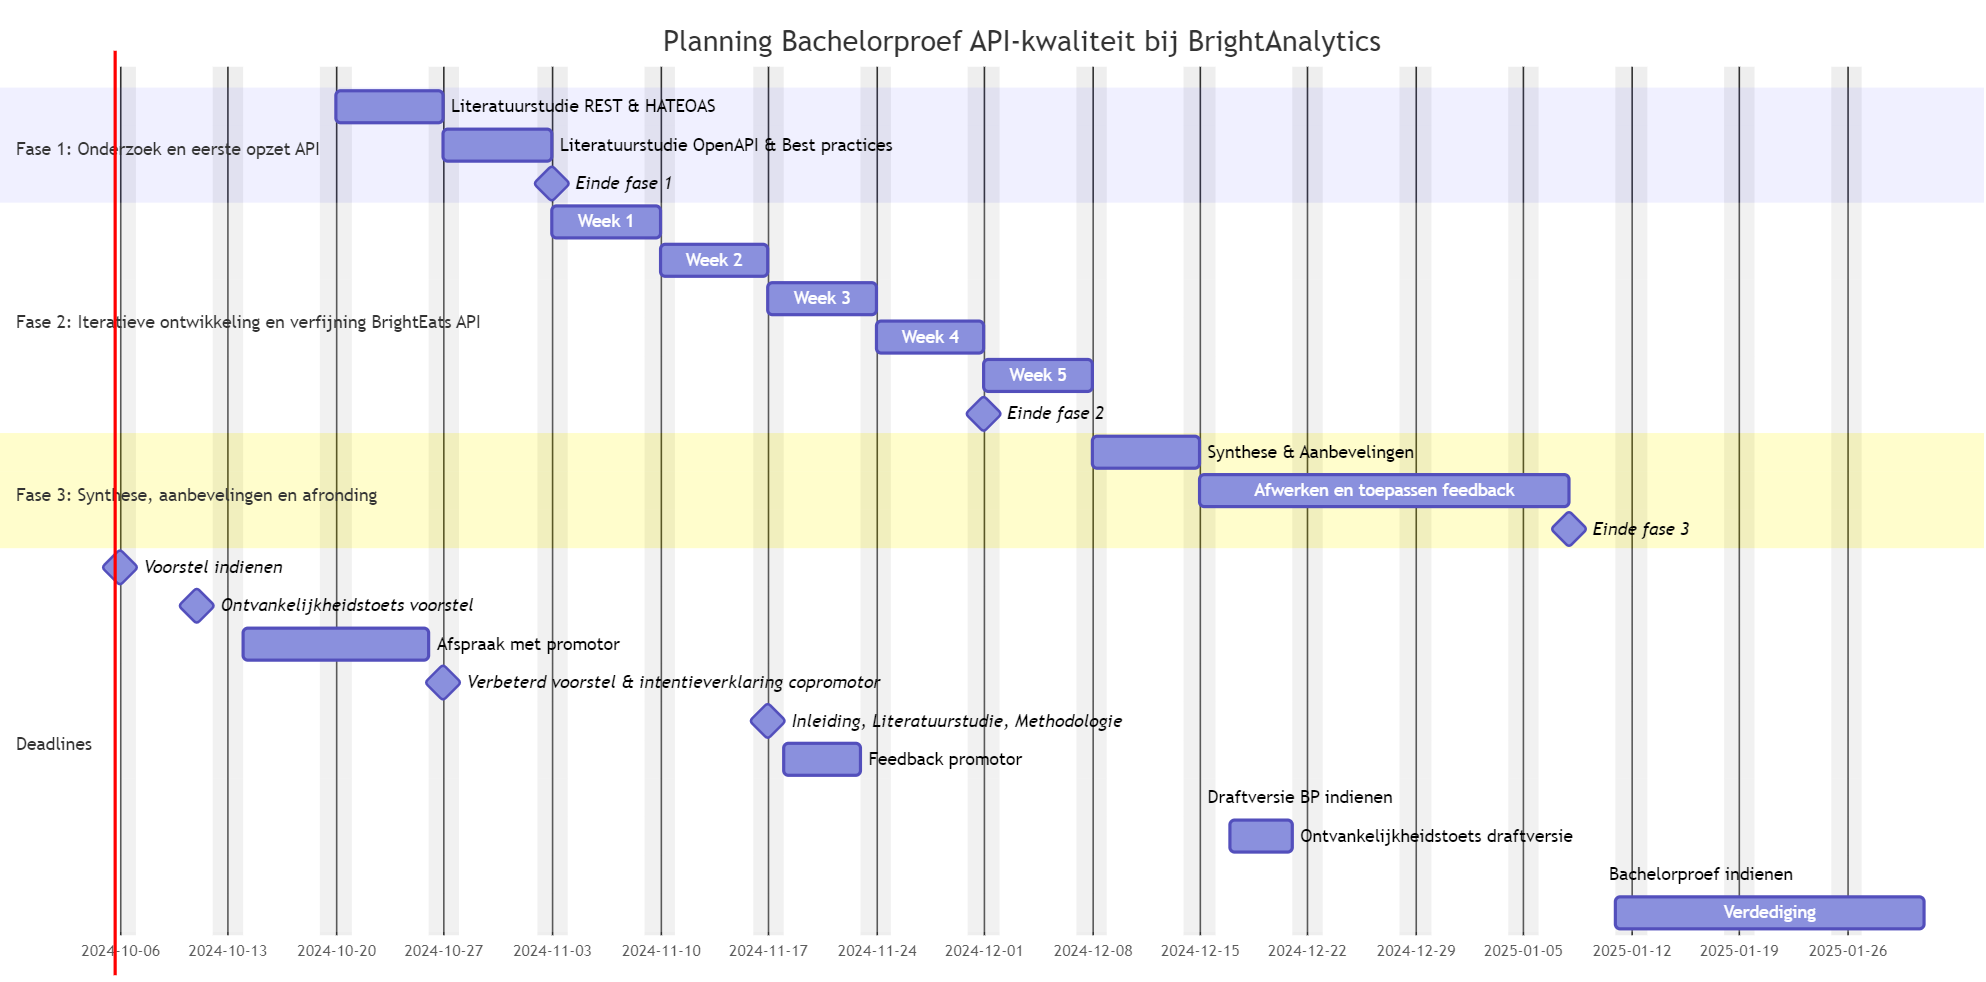
\includegraphics[width=\textwidth, keepaspectratio]{gantt-chart/gantt-chart.png}
  \caption{Gantt chart van de planning van de bachelorproef}
  \label{fig:gantt-chart}
\end{figure}


%%---------- Andere bijlagen --------------------------------------------------
% TODO: Voeg hier eventuele andere bijlagen toe. Bv. als je deze BP voor de
% tweede keer indient, een overzicht van de verbeteringen t.o.v. het origineel.
%\input{...}

%%---------- Backmatter, referentielijst ---------------------------------------

\backmatter{}

\setlength\bibitemsep{2pt} %% Add Some space between the bibliograpy entries
\printbibliography[heading=bibintoc]

\end{document}
